% ---- ETD Document Class and Useful Packages ---- %
\documentclass{ucetd}
\usepackage{subcaption,epsfig,amsfonts}
\usepackage{natbib}
\usepackage{amsmath}
\usepackage{amssymb}
\usepackage{amsthm}
\usepackage{mysty}

%% Use these commands to set biographic information for the title page:
\title{Data driven modeling of the low-Atwood single-mode Rayleigh-Taylor instability}
\author{Maxwell Hutchinson}
\department{Physics}
\division{Physical Sciences}
\degree{Doctor of Philosophy}
\date{December 9th, 2016}

%% Use these commands to set a dedication and epigraph text
\dedication{Dedicated to Tracey Ziev}


\begin{document}
%% Basic setup commands
% If you don't want a title page comment out the next line and uncomment the line after it:
\maketitle
%\omittitle

% These lines can be commented out to disable the copyright/dedication/epigraph pages
\makecopyright
\makededication


%% Make the various tables of contents
\tableofcontents
\listoffigures
\listoftables

\acknowledgments
% Enter Acknowledgements here

I would like to thank Robert Rosner for letting me chart my course through this thesis and my doctoral research more broadly.
I thank Aleksandr Obabko and Paul Fischer for supporting Nek5000 and working with me through the numerics.
I also thank Oana Marin and Michel Schanen for their excitement and Elia Merzari and Ron Rahaman for their support.
I thank Alexander Heinecke and Scott Parker for their help tuning the code to run on supercomputers.
I thank Elizabeth Hicks for helpful comments and advice.

For computer time, this research partially used the resources of the
Supercomputing Laboratory at King Abdullah University of Science \& Technology
 (KAUST) in Thuwal, Saudi Arabia.
This research used resources of the Argonne Leadership Computing Facility, which
is a DOE Office of Science User Facility supported under Contract DE-AC02-06CH11357.
I acknowledge support from the Department of Energy Computational Science graduate fellowship.

\abstract
% Enter Abstract here

The Rayleigh-Taylor instability is one of the most common and well studied phenomena in fluid dynamics.
Despite research dating to
the late 19th century, the non-linear dynamics
of the interfacial instability are still not fully understood, particularly in the case when the two fluids have nearly the same density.
It was recently demonstrated in this, the low-Atwood regime, that the idealized single-mode problem departs from established potential flow models in the form of a re-acceleration beyond the predicted terminal interface velocity.
This thesis is an attempt to model that re-acceleration and, more broadly, the late time dynamics of the single-mode low-Atwood Rayleigh-Taylor instability.

The approach taken here is based on buoyancy-drag models, which express a force balance between buoyancy and parasitic drag.
The dynamical buoyancy-drag model is supplemented with a mixing model that dilutes the buoyant force over time.
These models are written deliberately generally, with 8 unique coefficients.
Three of these coefficients are solved for by equating the early time behavior with that of well established linear theories.
The remaining 5 coefficients are estimated by relating them to drag coefficients, friction factors, and geometric ratios in the interface shape.

To evaluate the model and compute the 5 unknown coefficients more precisely, a set of direct numerical simulations are performed over the relevant parameter space.
These simulations are first validated against experimental data.
Then they are shown to converge and their resolutions are chosen such as to minimize computational cost given the accuracy scale of the model.
The 5 coefficients are fit to the resulting data set, and the model achieves better than 2\% error in the bubble height and 4\% error in the volume of mixed fluid.
Three coefficients are nominally independent of the parameterization of the problem, while two are shown to vary with the Rayleigh number and the diffusivity.


\mainmatter
% Main body of text follows

\chapter{Introduction}

\section{Formal definition}
The Rayleigh-Taylor instability occurs when the pressure and density gradients are in opposition:
\begin{equation}
(\nabla P)(\nabla \rho) < 0
\end{equation}
The canonical example of the Rayleigh-Taylor instability is a heavy fluid superposed over a lighter one in a gravitational field.
The standard terminology is based on this case.

Consider a horizontal planar interface at $z=0$ between a fluids of densities $\rho_h > \rho_l$ with the denser fluid at $z > 0$ and the lighter at $z < 0$, and a gravitational acceleration $-g \hat{z}$.
In equilibrium, the pressure must balance the gravitational force:
\begin{equation}
P(x,y,z) = \begin{cases}- \rho_h g z + C& \text{ if } z > 0 \\
                        - \rho_l g z + C& \text{ else}
           \end{cases}
\end{equation}
A small perturbation is introduced, moving some heavy fluid below the interface and some light fluid above it.
The forcing on the heavier fluid below the interface is:
\begin{equation}\elabel{force1}
\sum F = - \nabla P + F_g = \rho_l g  - \rho_h g < 0
\end{equation}
so the heavier fluid is forced downwards through the lighter fluid.
Conversely, the forcing on the lighter fluid above the interface is:
\begin{equation} \elabel{force2}
\sum F = - \nabla P + F_g = \rho_l g  - \rho_h g > 0
\end{equation}
so the lighter fluid is forced upwards through the heavier fluid.
Perturbations in the interface grow, so the configuration is unstable.

\section{Instances and motivation}
The Rayleigh-Taylor instability is present in both natural and constructed systems at many scales.
This section describes a few such systems of particular importance.

\paragraph{Supernovae}
One of the earliest motivations for the study of the Rayleigh-Taylor instability comes from the stability 

\paragraph{Salt fingers}
Salt fingers are an instance of the Rayleigh-Taylor instability set up by a difference in the diffusivity of two mass carriers, in this case salinity and temperature.

\paragraph{ICF}
Inertial confinement fusion (ICF) is a fusion technique that confines hot dense plasma temporarily via an implosion, rather than magnetic field lines.
In ICF, the cryogenic hydrogen is coated with a plastic ablator forming very small hollow spheres, or microcapsules.
The microcapsules are through a cylindrical hohlraum.
When the capsule is at the center of the hohlraum, the hohlraum is illuminated with a high energy burst of laser light and radiates x-rays.
The x-ray radiation is absorbed by the plastic ablator causing it to rapidly expand and blow off the microcapsule, creating an implosion in the hydrogen fuel.

The implosion isn't perfectly uniform; the x-ray radition provides non-uniform acceleration and there are asymmetries in the microcapsue.
These perturbations are Rayleigh-Taylor unstable: the dense plastic ablator is being accelerated through lighter hydrogen fuel.
The carbon in the ablator is much better at radiating energy than the hydrogen, so as the RTI mixes the plastic into the fuel the fuel cools, preventing ignition.

\paragraph{Reactors}


\section{Terminology}

\paragraph{Atwood number}
The Atwood number characterizes the density contrast:
\begin{equation} \elabel{atwood}
A = \frac{\rho_1 - \rho_2}{\rho_1 + \rho_2} \in (-1,1)
\end{equation}
where $\rho_1 > \rho_2$ corresponds to positive Atwood number.

There are three distinct regimes for the Atwood number: high, low, and moderate.
At high Atwood number, e.g. air and water, the internal dynamics of the light fluid are decoupled from the heavy fluid.
The transfer of momentum through the interface into the dense fluid can be neglected.
In this regime, potential flow models are reasonable.

At low Atwood number, e.g. salt water and fresh water, the governing equations can be linearized about the Atwood number, leading to the Boussinesq approximation.
The behavior of the bubbles and spikes are identical.

At moderate Atwood number, e.g. oil and water, not only is enough vorticity is generated to invalidate potential flow models but also the density difference breaks bubble-spike symmetry.

\paragraph{Boussinesq approximation}
If the density contrast, $\Delta \rho$ is small compared to the average density $\bar{\rho}$, then 
the governing equations can be linearized with respect to density.
This is known as the Boussinesq approximation and has the primary effect of neglecting differences in the inertia of the two fluids.

\paragraph{Constant property}
In the spirit of the Boussinesq approximation, which neglects differences in the inertial of the two fluids, we furhter assume the two fluids share all other material properties, such as viscosity.

\paragraph{Miscible interface}
In most cases where the Boussinesq and constant property approximations are valid, the interface between the two fluids is miscible.
For example, low-concetration solutions in a common solvent have interfaces governed by a diffusion coefficient, $D$, and small temperature graidents are governed by a thermal diffusivity $\alpha$.
In the limit where $D$ or $\alpha$ goes to zero, the interface is immiscible but there is no surface tension.

\paragraph{Single-mode}

\paragraph{Multi-mode}

\paragraph{Governing equations}
Given a miscible interface between two Boussinesq,  constant property fluids, the governing equations can be recaste in terms of an active scalar:
\begin{align}
\der{u}{t} + u \cdot \nabla u &= \nu \nabla^2 u - \nabla P - A g \phi \hat{z}\\
\der{\phi}{t} + u \cdot \nabla \phi &= D \nabla^2 \phi \\
\nabla \cdot u  &= 0
\end{align}
These equations have three governing parameters; $Ag$, $\nu$, and $D$; which admit the construction of two dimensionless numbers:
\begin{equation}
\text{Grashof} = \frac{Ag L^3}{\nu^2}
\end{equation}
\begin{equation}
\text{Schmidt} = \frac{\nu}{D}
\end{equation}
If the initial and boundary conditions can be characterized by a single length scale, then these two parameters uniquely identify the system.

\paragraph{Bubble height / spike depth / mixing width}

Experiment and theory focus on the observation and explanation of a set of observables that are much smaller than the full degrees of freedom of the system.
The selection of these observables is informed by practical aplication and methodological analogy.


The bubble height refers to the distance beyond the initial interface that the bubble front has traveled, as a function of time.
The standard experimental definition projects the density onto a line normal to the initial interface and defines the front interface as the point at which the density is at its 99th or 95th percentile.
More formally:
\begin{equation}
H[\epsilon] = \sup \left\{z : \int dx dy \rho(x,y,z) < (1-\epsilon) \int dx dy \rho(x,y,\infty) \right\}
\end{equation}



\begin{comment}
\section{Stages}

\subsection{Linear growth} 
When the amplitude of the surface perturbation is small compared to its wave-length, the perturbation grows exponentially.
The growth rate is seen to depend on the forcing, wave-length, viscosity, diffusivity, and interface thickness.
This stage can be treated with linear and weakly-nonlinear theories, as discussed further in \sref{linear}.


\subsection{Single-mode stagnation}
As the growing Rayleigh-Taylor modes saturate, the acceleration of the bubble tip decreases.
The stagnation stage of the single-mode Rayleigh-Taylor instability is defined as a stage of the flow that exhibits nearly constant bubble velocity.
It had been believed that the first such stage was terminal, i.e. steady state.
It has recently been shown, via both simulation~\cite{Ramaprabhu2006} and experiment~\cite{Wilkinson2007}, that at low Atwood number and high Reynolds number the flow continues to develop into re-acceleration stage.
For this reason, the nearly constant velocity is termed the \textit{stagnation velocity}.
The primary observable of a stagnation stage is the stagnation velocity, but there is secondary interest in the velocity profile through the transition from the weakly non-linear to stagnation stages and in the bubble height at which stagnation velocity is reached.

\subsection{Single-mode late time}
For low Atwood and high Reynolds numbers, the stagnation stage is followed by a reacceleration stage around unity aspect ratio.
Reacceleration has been seen in both numerical simulations \cite{Ramaprabhu2006, Ramaprabhu2012, Wei2012} and experiments{Wilkinson2007}.
Following the immediate reacceleration, there is disagreement as to whether or not the single mode problem ultimatly reaches a terminal stage.
Ramaprabhu \etal suggest that the re-acceleration is transient, with the bubble velocity ultimately returning to a potential-flow-like value.
Wei and Livescu, on the other hand, suggest the terminal stage to be one of `chaotic development` with quadratic growth dynamics.
Unfortunately, the late-time stages have yet to be accessed experimentally.

\subsection{Multi-mode}
Under natural multi-mode initial conditions, the linear growth modes couple as the aspect ratio increases, forming bubble and spike structures.
The bubbles and spikes interact with one another, competetively and constructively, leading to successively larger structures.
It is generally observed that the multi-mode aspect ratio, $D_b / h$, remains nearly constant.
\end{comment}
 % Introduction

\chapter{Background}

The study of the Rayleigh-Taylor instability is primarily interested in evolution of the interface, that is the rate of penetration of the light fluid into the dense one and vice versa.
While the volumetric mixing rate is relevant in some contexts, most flows have relatively low diffusivities, i.e. high Prandtl and Schmidt number, so mixing is dominated by transport rather than diffusion.

In this section, we review approaches to modeling the evolution of the interface and experimental efforts to validate those models.


\section{Linear and weakly non-linear models} %\slabel{linear}

The earliest models of the Rayleigh-Taylor instability were based on a linearization of the governing equations about the interface.
Recently, with the aid of computational algebra, it has become possible to retain higher order terms in the expansion, demonstrating the coupling between different modes.
However, even high order expansions fail as the interface loses analyticity.

\subsection{Lord Rayleigh's linear model}

Lord Rayleigh considered a sinusoidal perturbation of an incompressible, inviscid, immiscible, quiescent stratified interface~\cite{Rayleigh1883}.
When the amplitude is small compared to the wavelength, the continuity and momentum equations can be linearized.
\begin{align}
\left(\bar\rho + \tilde\rho\right) \left[\der{u}{t} + u \nabla u \right] &= - \nabla{\tilde{P}} + g(\bar\rho + \tilde\rho)\\
\nabla \cdot u &= 0 \\
\end{align}
where $u, \tilde\rho, \tilde{P}$ are small and their products neglected.
The solution is an exponential with a growth rate:
\begin{equation} \elabel{simple_growth}
  \gamma^2 = A g k 
\end{equation}
where $g$ is the acceleration experienced by the fluid, and
$k = 2 \pi / \lambda$ is the wave-number of the perturbation.
Positive Atwood numbers correspond to unstable density stratifications, which grow exponentially.
Negative Atwood numbers correspond to stable density stratifications, which oscillate.
For a derivation of \eref{simple_growth}, see \aref{LST}.

\subsection{Viscous and diffusive linear models}
Chandrasekhar~\cite{Chandrasekhar1955} and Hide~\cite{Hide1955} generalized the linear theory to viscous fluids by including an isotropic incompressible Newtonian shear stress.
Chandrasekhar worked out the constant property, $\mu_1 = \mu_2$ case and Hide included an approximate combination of distinct viscosities.
Here, we are concerned with the simpler constant propety case:
\begin{equation} \elabel{visc_growth}
  \gamma = \sqrt{A g k + \nu^2 k^4} - \nu k^2
\end{equation} 
where 
$\nu$ is the kinematic viscosity.

LeLevier et al.~\cite{LeLevier1955} generalized the linear theory to continuous density gradients, specifically exponentially smoothed profiles for the form $\bar\rho \pm e^{\mp K z} \delta\rho$.
\begin{equation}
\gamma = \sqrt{\frac{A g k K}{k + K}}
\end{equation}

Duff \etal~\cite{Duff1962} generalized the linear theory to miscible interfaces and incorporated Chandrasekhar and Hide's viscous theories, producing an combined expression for the growth rate:
\begin{equation} \elabel{duff_simple}
\gamma = \sqrt{\frac{A g k}{\psi(A,k\delta)} + \nu^2 k^4} - (\nu + D) k^2
\end{equation}
where 
$\delta$ is the instantaneous interface thickness,
$D$ is the diffusivity,
and $\psi$ is a function of the Atwood number and the product of the wavenumber and the interface thickness.
For $k \delta \lesssim 1$ and $A << 1$, $\psi \approx 1 + k \delta / \sqrt{\pi}$.

In the constant propety case, $\delta = 2 \sqrt{D t}$, introducing a time-dependence on the linear stability:
\begin{equation} \elabel{duff_growth}
\gamma = \sqrt{\frac{A g k}{1 + \frac{2 k}{\sqrt{\pi}}\sqrt{D t} } + \nu^2 k^4} - (\nu + D) k^2
\end{equation}

\subsection{Weakly nonlinear expansions}
Jacobs and Catton provide a third order weakly non-linear theory for the inviscid unit Atwood Rayleigh-Taylor instability~\cite{Jacobs1988}.
Their weakly non-linear theory is primarily used to compare linear growth rates across a variety of perturbation symmetries in 3D.
In particular, hexagonal and axi-symmetric perturbations are found to grow faster than rectangular perturbations.

Berning and Rubenchik extend the theory to arbitrary Atwood immiscible flows at higher order, but take only the third order~\cite{Berning1998}.
They perform a similar geometric comparison to Jacobs and Catton, but also use the harmonic couplings to characterize linear saturation.

The perturbation expansion has been taken to at least the 10th order by Liu \etal~\cite{Wang2010}.
However, there is limited progress to be made with such expansions, as singularities with branching point structures develop at moderate bubble displacements~\cite{Berning1998}.
Put another way, the interface and velocity potentials are not analytic in the span-wise position, e.g. when the interface rolls up.

\section{Potential flow models}

The next class of models to be applied to the Rayleigh-Taylor instability are potential flow models.
These models assume that little vorticity is generated and that it is confined to the interface, which is true at high Atwood numbers.

\subsection{Layzer's unit Atwood model}

One of the first such models is due to Layzer~\cite{Layzer1955}.
Layzer's model is of an bubble with $\rho = 0$ rising in a fluid of density $\rho = 1$ ($A = 1$).
The bubble and fluid are assumed to be incompressible and inviscid.
The flow begins at rest, so there is no initial vorticity.
Layzer claims the flow will therefore continue to be irrotational, because the viscous generation term of the vorticity equation is zeroed for inviscid, incompressible flows.

Since the flow is inviscid and irrotational, Layzer uses the potential flow technique, writing the velocity as the gradient of a scalar potential:
\begin{equation}
v = \nabla \phi
\end{equation}
where 
$v$ is the velocity and 
$\phi$ is the scalar potential.
Incompressibility zeroes the Laplacian of the potential:
\begin{equation}
\nabla^2 \phi = 0
\end{equation}
A Bernoulli equation is used model the interface:
\begin{equation} \label{eqn:LayzerBernoulli}
\der{\phi}{t}(\eta(r,t), r, t) - \frac{1}{2} \left(\left(\pder{\phi}{z}\right)^2(\eta(r,t), r, t) +\left(\pder{\phi}{r}\right)^2(\eta(r,t), r, t)\right) - g \eta(r,t) = f(t)
\end{equation}
where 
$\eta(r,t)$ is the height of the interface,
$g$ is the gravitational acceleration, and 
$f(t)$ is an arbitrary function of time but not space.
The flow is axially symmetric with a vanishing radial component at transverse walls and vanishing vertical component far away from the bubble:
\begin{equation}
\pder{\phi}{r}(z,R,t) = 0 \qquad \pder{\phi}{z}(\pm \infty, r, t) = 0
\end{equation}
Finally, the fluid advects the interface:
\begin{equation}
\der{\eta}{t}(r,t) = \pder{\phi}{z}(\eta(r,t), r, t) - \pder{\phi}{r}(\eta(r,t), r, t) \der{\eta}{r}(r,t)
\end{equation}

The details of the derivation can be found in \aref{Layzer} and the results are summarized here.
The stagnation velocity in two and three dimensions, assuming axial symmetry in the latter case, are:
\begin{equation}
V_{2d} = \frac{1}{\sqrt{3}} \sqrt{\frac{g R}{\pi}}  \qquad V_{cyl} = \sqrt{\frac{g R}{\beta_1}} 
\end{equation}
where $\beta_1$ is the first root of the first order Bessel function of the first kind: $J_{1}(\beta_1) = 0$.

\subsection{Goncharov's high Atwood model}

Goncharaov extends the Layzer model to include two fluids of arbitrary density difference and makes a different choice of simplifying approximation for the Bernoulli equation~\cite{Goncharaov2002}.
The consideration of a second fluid with non-zero density turns the Bernoulli equation \eref{LayzerBernoulli} into a difference:
\begin{equation} \label{eqn:GonBernoulli}
\begin{aligned}
&\der{\phi}{t}(\eta(r,t), r, t) - \frac{1}{2} \left(\left(\pder{\phi}{z}\right)^2(\eta(r,t), r, t) +\left(\pder{\phi}{r}\right)^2(\eta(r,t), r, t)\right) - g \eta(r,t) \\
&= f(t) \\
\end{aligned}
\end{equation}
The Goncharaov model keeps the free-slip boundary condition between the two fluids, which is exact only for $A = 1$ and a reasonable approximation for $\rho_1 / \rho_2 >> 1$.
In this respect, Goncharaov's should be reasonable for high-Atwood, high-Reynolds number flows.

The assumption that the flow is irrotational applies only at high Atwood number.
At moderate and low Atwood numbers, secondary Kelvin-Helmholtz (KH) instabilities develop at the vertical sheer layer separating the two fluids~\cite{Ramaprabhu2006,Wilkinson2007}.
The effects of the vorticity in the lighter fluid were addressed theoretically by Banerjee et al~\cite{Banerjee2011} and numerically by Ramaprabhu et al.~\cite{Ramaprabhu2012}.

\subsection{Abarzhi and Sohn's models}

\subsection{Departure from potential flow}

\subsection{Banerjee's rotational model}

\cite{Banerjee2011}

\section{Buoyancy-drag models}

Buoyancy-drag models were developed concurrently with potential flow models, in part to provide a physical interpretation for their results.
They balance buoyant and parasitic forces related to the geometry of a model bubble.
Historically, buoyancy-drag models have had only 1 or 2 adjustable parameters, so they are evaluated more on their ability to reproduce specific features of the flow, e.g. the terminal velocity, rather than the full time-history.
Here, we focus on models applicable to single-mode non-interacting bubbles.

\subsection{Bubble model of Davies and Taylor}

Early experiments on the Rayleigh-Taylor instability by Davies and Taylor~\cite{Davies1950a} were performed by measuring the dynamics of large bubbles of gas rising through a dense liquid.
In their analysis, they relate the terminal velocity of the bubble to a drag coefficient, implicitly defining a bouyancy-drag model of the form:
\begin{equation} \elabel{dtbd}
\dot{v} \rho \mathcal{V} = \rho g \mathcal{V} - C_D \pi D^2 \frac{1}{2} \rho v^2,
\end{equation}
where $v$ is the gas bubble velocity,
$\rho$ is the density of the liquid,
$g$ is the gravitational acceleration,
$\mathcal{V}$ is the bubble volume,
$C_D$ is a drag coefficient, and
$D$ is the bubble diameter.

%also \cite{Alon1995}

\subsection{Tube model of Dimonte and Schneider}

Dimonte and Schneider develop a buoyancy-drag model for tube-shaped bubbles~\cite{Dimonte1996,Dimonte2000a} based on Davies and Taylor's model, \eref{dtbd}.
They let the ratio of the area to the volume go with the inverse bubble height, $\mathcal{A} / \mathcal{V} \sim 1/h$.
They also add a rescaling of the buoyant term by $\beta$, attributed to Youngs:
\begin{equation}
\dot{v_b}  = \beta A g - C_d \frac{v_b^2}{h_b}, 
\end{equation}
where $v_b$ is the bubble velocity,
$\beta < 1$ accounts for the relatively smaller buoyant portion of the bubble due to entrainment,
$C_d$ is a drag coefficient, and
$h_b$ is the bubble height.
$\beta$ and $C_d$ depend on the Atwood number, but Dimonte proposes $\beta = 1/2$ and $C_d = 2$ for $A << 1$~\cite{Dimonte2000}.
However, the model is stated to apply to self-similar bubble fronts.

\subsection{Self-similar model of Oron}

A simple model of the stagnation stage is buoyancy-drag~\cite{Oron2001}:
\begin{equation} \elabel{buoyancy_drag}
(\rho_1 + C_a \rho_2) \mathcal{V} \ddot{h} = (\rho_2 - \rho_1) \mathcal{V} g - C_d \dot{h}^2 \rho_2 \mathcal{A}
\end{equation}
where $\rho_2 > \rho_1$ are the densities of the two fluids, 
$C_a$ is an added mass coefficient,
$\mathcal{V}$ is the volume of the bubble, 
$h$ is the height of the bubble,
$g$ is the gravitational acceleration,
$C_d$ is a drag-like coefficient, and
$\mathcal{A}$ is the bubble surface area.
There is ambiguity as to the value of un-subscripted $\rho$, but in the low Atwood number limit $\rho_1 \approx \rho_2 = \rho$ removes it:
\begin{equation}
\ddot{h} = A g - \frac{C}{2} \dot{h}^2 \frac{\mathcal{A}}{\mathcal{V}}
\end{equation}

There are two length scales in the single mode instability: $\lambda$ and $h$.
If the bubble is self-similar or unsupported, as is generally the case in the literature, then $\mathcal{A}/\mathcal{V} \sim 1/\lambda$.
Rolling that constant into $C$ yields:
\begin{equation} \elabel{bouancy_drag}
\ddot{h} = A g - C \frac{\dot{h}^2}{2 \lambda}  
\end{equation}
The stagnation velocity is therefore:
\begin{equation}
v_s = \sqrt{\frac{2 A g \lambda}{C}}
\end{equation}
This motivates the definition of the Froude-type number:
\begin{equation}
\text{Fr} = \frac{v}{\sqrt{\frac{A g \lambda}{1+A}}} \xrightarrow{A << 1} \frac{v}{\sqrt{A g \lambda}}
\end{equation}
which relates to the drag-like coefficient as:
\begin{equation}
\text{Fr} = \sqrt{\frac{2}{C}}
\end{equation}


\section{Problems with single mode buoyancy-drag models}

It has recently been shown, via both simulation~\cite{Ramaprabhu2006} and experiment~\cite{Wilkinson2007}, that at low Atwood number and high Reynolds number the flow continues to develop beyond the terminal velocity predicted by potential flow and buoyancy-drag into re-acceleration stage.
For this reason, the nearly constant velocity is termed the \textit{stagnation velocity}.

The desire to describe this re-acceleration process, quantitatively, is the motivation for this thesis.
However, I will first give two qualitative explanations for while re-acceleration should be expected: one based on the pressure balance and another by identifying a historical inconsistency in the development of buoyancy-drag models.

\subsection{Pressure in the single-mode RTI}

If there is a terminal velocity regime, can it be due to form drag?
Let $\nu \rightarrow 0$ and consider a fluid element lying on the axis
of a bubble or spike.
By symmetry, it will only have a z-component of the velocity.
The z-forces must balance:
$$ \rho \phi g = \pder{P}{z} $$
In the finger, the pressure would be decreasing with $z$.
In the bubble, the pressure would be increasing with $z$.
There would necessarily be a pressure gradient between the head of the finger and the tail of the bubble, and vice versa.
As the aspect ratio exceeded unity, the span-wise pressure gradient would exceed the gravitational forcing.
The resulting span-wise flow would rapidly mix the two fluids, destroying the bubble and spike.

The form of the bubble and spike require the pressure to be reasonably homogeneous span-wise.
Only at the bubble and spike tips do we accept a span-wise flow: the displacement of stationary fluid by the tip.
In other words, the pressure drag is highly localized to the bubble and spike tips.
The flow from tail to tip is attenuated predominately by viscous drag.

\subsection{Historical inconsistency}

The buoyancy-drag model model contains a buoyant term that goes with the bubble volume and a form drag term that goes with the bubble's area.
The model was originally developed to describe multi-mode self-similar flow, in which there is only one length scale, the dominant wavelength $\lambda$.
Consequently, the ratio fo the volume to the surface area is $\lambda^{-1}$, yielding a terminal velocity as a function of $\lambda$.

However, the single-mode RTI has two length scales: in addition to the wavelength $\lambda$ there is the bubble height, $h$.
In other words, single-mode RTI bubbles are cylindrical instead of spherical with an axis length that goes with the bubble height.
The ratio of the volume to surface area is $h^{-1}$, not $\lambda^{-1}$, so there is no terminal velocity.
Only by introducing a drag term that goes with the height $h$, such as skin drag, can a terminal velocity be recovered.
This terminal velocity would be a function of the viscosity, and therefore cannot be described by potential flow.

 % Introduction

\chapter{Standalone papers}

This thesis contains three standalone papers.
They are logically ordered from the top down.

The first paper contains a new buoyancy-drag model developed to describe the late time behavior in the low-Atwood, moderate Grashof case.
It contains model coefficients that are fit to a data set of direct numerical simulations.
This single author paper will be submitted to for peer review.

The second paper validates those direct numerical simulations against experimental data from Wilkinson and Jacobs~\cite{Wilkinson2007}.
This establishes that the simulations contain the physical processes responsible for re-acceleration and other unexplained late-time phenomena.
The paper takes advantage of the generality of numerical data to explore feature of the flow that were not available to the original experiment, namely the interaction between the bubbles and pressure driving secondary flows in the mid-plane.
This single author paper has been submitted to peer review.

The third paper contains a performance and convergence study of the numerical method and simulation software with the single mode Rayleigh-Taylor problem as a benchmark.
The NekBox code, which was specialized specifically to this project, is shown to be an efficient tool for performing these calculations.
Furthermore, the resolution is selected such that the simulation error is an order smaller than the expected model error, which ensures that the flow is sufficiently but not over resolved.
Maxwell Hutchinson authored all of sections 2 and 4 and the majority of sections 1 and 5.
This paper has been peer reviewed and published in the proceedings of the International Conference on High Performance Computing (ISC).



\chapter{Data-driven modeling of the low-Atwood single-mode Rayleigh-Taylor instability}

\section{Abstract}

The Rayleigh-Taylor instability (RTI) pervades classical fluid dynamics and is essential to a diversity of phenomena, e.g. salt fingers, thermonuclear flames, and inertial confinement fusion, but remains poorly understood in dissipative systems.
Recently, the single-mode RTI has shown experimentally and numerically to deviate from established potential flow models when the Atwood number was less than $1/2$.
Attempts to explain the deviation, termed re-acceleration, have been ad-hoc and hindered by a dearth of data at late times and high aspect ratios.
This paper present buoyancy-drag and mixing models that include dissipative terms and match the linear theory.
To inform the model, a numerical experiment is performed, simulating a range of Grashof and Schmidt numbers and reaching bubble heights 34$\times$ the bubble width.
The model coefficients are estimated by physical argument and then fit to the numerical results.
The model error is less than 2\% for the bubble height and 4\% for the volume of mixed fluid.
An attempt is made to interpret variations in the fit parameters with the Rayleigh and Schmidt numbers, where present, but it is hindered by many of the simulations interacting with the boundaries.
Simulations in higher aspect ratio domains would improve the model.

\section{Introduction} \slabel{intro}

The Rayleigh-Taylor instability has been the subject of considerable study since its characterization by Lord Rayleigh in the 19th century~\cite{Rayleigh1883}.
Despite this, many aspects of the non-linear growth remain poorly understood.
Analytic models based on potential flow have been reasonably effective for flows with a large density jump, \ie an Atwood number, $\Delta \rho / \sum \rho$, near unity~\cite{Layzer1955, Layzer1955}.
However, recent experiments at low Atwood number have demonstrated a significant departure from the potential flow limit:
Rayleigh-Taylor bubbles are seen accelerating past the terminal velocity predicted by potential flow models~\cite{Wilkinson2007}.
The acceleration persists beyond times which are experimentally accessible, so numerous efforts have been made to compute the late time flow numerically~\cite{Ramaprabhu2012,Wei2012}.
Ultimately, the goal is to use these numerical experiments to inform a simple model that captures the key features and mechanisms of the flow, as potential flow models do for high Atwood number flows.

This study concerns the dynamics of the single-mode Rayleigh-Taylor instability (smRTI), where the interface between a heavy fluid and a light fluid is perturbed with a single wavelength $\lambda$ and corresponding wavenumber $k$.
If the Atwood number is low, then at early times the interface grows exponentially with a rate given by a linear approximation~\cite{Duff1962}:
\begin{equation} \elabel{duff0}
\gamma = \sqrt{\frac{A g k}{1 + \pi^{-1/2} k \delta} + \nu^2 k^4} - (\nu + D) k^2,
\end{equation}
where $A$ is the Atwood number,
$g$ is the local acceleration,
$\delta$ is the interface thickness,
$\nu$ is the kinematic viscosity, and
$D$ is the diffusivity.
As the amplitude approaches the wavelength, the linear growth saturates.
At unit Atwood number, the non-linear regime is described by potential flow, in which Layzer~\cite{Layzer1955} found the interface approaches a terminal velocity proportional to the root of the acceleration and wavelength: $v_L \sim \sqrt{g \lambda}$:
Potential flow models have been extended to $A < 1$, with the most successful model by Goncharov~\cite{Goncharov2002}:
\begin{equation} \elabel{goncharov}
v_G = \frac{1}{\sqrt{\pi}} \sqrt{\frac{A g \lambda}{1+A}}
\end{equation}

Experiments by Wilkinson and Jacobs~\cite{Wilkinson2007} show that after reaching the velocity given by \eref{goncharov}, low Atwood bubbles unexpectedly accelerate a second time.
This is termed `re-acceleration`, with the terminal velocity replaced by a `stagnation velocity`.
Re-acceleration was not present in popular potential flow and buoyancy-drag models, and attempts to capture re-acceleration have been the emphasis of recent model development in the low Atwood number regime.

Experiments have thus far been unable to observe more than the onset of the re-acceleration phase.
Therefore, the community has turned to numerical studies to compute late-time dynamics.
At least two such efforts have been undertaken, one by Ramaprabu \etal~\cite{Ramaprabhu2012} and one by Wei and Livescu~\cite{Wei2012}, leading to slightly different conclusions.
In the study by Ramaprabhu, the flow accelerates to around twice the stagnation velocity and then decelerates back to the stagnation velocity, indicating that re-acceleration may be a transient.
In the study by Wei and Livescu, the flow re-accelerates and then breaks up into many small pockets of buoyant fluid, which themselves continue to accelerate at nearly a fixed rate.

Buoyancy-drag models have been proposed for the multi-mode and single-mode dynamics of the bubble front.
They balance the buoyant force of the bubble with a drag force to predict the front velocity as a function of the characteristic length.
Ramaprabhu proposes an additional forcing term based on the development of a vortex ring at the bubble tip, but relies on observation of the mean vorticity experimentally or in numerical simulations.
There is a need for a predictive model for re-acceleration that relies only on the initial conditions.

In \sref{model}, we propose a simple buoyancy-drag model for the dynamics of the smRTI.
In \sref{exp}, we present a battery of numerical trials.
In \sref{late}, we describe the regimes present in late time bubble trajectories.
In \sref{fit}, we fit the unconstrained model coefficients to the numerical results..
Finally, in \sref{conc}, we assess the current state of smRTI and highlight outstanding questions.



\section{Simple model} \slabel{model}

We base our model on the buoyancy-drag models of \cite{Oron2001}:
\begin{equation}
(\rho_1 + \rho_2) \mathcal{V} \ddot{h} = (\rho_2 - \rho_1) g \mathcal{V} - C \dot{h}^2 \rho \mathcal{A},
\end{equation}
where $\rho_1$ and $\rho_2$ are the densities of the light and heavy fluid,
$\mathcal{V}$ is the characteristic volume of the bubble
$g$ is the acceleration,
$C$ is a drag-like coefficient, and
$\mathcal{A}$ is the characteristic cross sectional area of the bubble.
Making the Boussinesq approximation, $\rho_1 \approx \rho_2$ yields:
\begin{equation}
\ddot{h} = A g - \frac{C}{2} \dot{h}^2 \frac{\mathcal{A}}{\mathcal{V}}.
\end{equation}
In the self-similar regime there is only one length scale, so $\mathcal{A}/\mathcal{V} \sim 1 / \lambda$.
However, in the single-mode regime that is the focus of this study, the bubbles are elongated, producing two length scales: a span-wise scale $\lambda$ and a stream-wise scale $h$.
Therefore, for the smRTI $\mathcal{A}/\mathcal{V} \sim \frac{1}{h}$ and the model of Oron \etal yields unbounded velocities:
\begin{equation}
\ddot{h} = A g - \frac{C}{2} \frac{\dot{h}^2}{h}.
\end{equation}
Because the strength of the form drag relative to buoyancy decreases at high aspect ratio, we must consider other drag terms, such as skin drag, that grow at least linearly with $h$.

\subsection{Dynamics}

We begin by listing the external forces the bubble experiences.  The first is the buoyant force:
\begin{equation}
F_b = C_0 A g \lambda^2 h,
\end{equation}
where $C_0$ is an unknown coefficient.
The next is the form drag:
\begin{equation}
F_f = C_1 \lambda^2 \dot{h}^2,
\end{equation}
where $C_1$ is similar to a drag coefficient.
The next is the viscous, or skin, drag:
\begin{equation}
F_s = C_2 \nu h \dot{h},
\end{equation}
where $C_2$ is another unknown coefficient and 
$\nu$ is the kinematic viscosity.

To complete the dynamic equation, we must characterize the inertia of the bubble.
The bubble is roughly cylindrical with a height $h$, so we expect an inertial term of the form $\lambda^2 h$.
However, consider the limit of $h \rightarrow 0$.  
Here, streamlines must extend from bubble to spike, which has a characteristic separation $\lambda$ for an inertial term of the form $\lambda^3$.
Therefore, we expect the inertia to be a mix of a term that goes as $\lambda^2 h$ and one that goes as $\lambda^3$:
\begin{equation} \elabel{inertia}
I = C_3 \lambda^2 h + C_4 \lambda^3,
\end{equation}
where $C_3$ and $C_4$ are two more unknown coefficients.

The complete dynamic equation is:
\begin{equation}
\ddot{h} = \frac{C_0 A g \lambda^2 h - C_1 \lambda^2 \dot{h}^2 - C_2 \nu h \dot{h}}{C_3 \lambda^2 h + C_4 \lambda^3}.
\end{equation}
Without loss of generality, we can let $C_0 = 1$ and simplify:
\begin{equation} \elabel{dynamics}
\ddot{h} = \frac{A g h - C_1 \dot{h}^2 - C_2 \nu (h/\lambda^2) \dot{h}}{ C_3 h + C_4 \lambda }.
\end{equation}
We can non-dimensionalize by defining a dimensionless length and time:
\begin{equation}
z = \frac{h}{\lambda}, \qquad \tau = \sqrt{\frac{A g}{\lambda}} t,
\end{equation}
which simplifes:
\begin{equation}
\ddot{z} = \frac{z - C_1 \dot{z}^2 - C_2 \text{Gr}^{-1/2} z \dot{z}}{C_3 z + C_4},
\end{equation}
where
the derivative is with respect to $\tau$ and 
$\text{Gr} = A_0 g \lambda^3 \nu^{-2}$ is the Grashof number.


\subsection{Mixing}

As the bubble height grows, the velocity approaches a terminal value specified by the balance between buoyancy and skin drag.
At terminal velocity, the flux of pure fluid into the bubble is bounded.
However, the interfacial mixing continues to grow with the interfacial area, which grows with $h$.
Therefore, for any finite diffusivity, the bubble will ultimately diffuse away.
For this reason, we must include the effects of interfacial mixing, at least to the first order.

The quantity of mixed fluid, $m$ is computed directly from the time, bubble height, diffusivity, and initial interface thickness.
The quantity of mixed fluid is defined as the integral of the absolute value of the scalar:
\begin{equation}
	m(t) = \int \left( 1-\text{abs}\left[\phi(x,y,z,t)\right] \right) dV,
\end{equation}
where we assume the mean scalar is zero, $\int \phi dV = 0$.

We approximate the volume integral by a 1D integral across the interface multiplied by the surface area:
\begin{equation}
	m(t) \approx S \int \left( 1- \text{abs}\left[\phi_1(r)\right] \right) dr,
\end{equation}
where $S$ is the surface area and
$\phi_1$ is a model 1D scalar profile:
\begin{equation}
\phi_1(r) = \frac{1}{2} \left( \erf\left[\frac{r}{\delta}\right] - \erf\left[\frac{r - d}{\delta}\right] \right),
\end{equation}
where $\delta$ is the interface width and
$d$ is the diameter of the bubble.

The surface area has contributions from the bubble tip and side walls:
\begin{equation} \elabel{surface_area}
S = \left(C_6 \lambda^2 + C_5 \lambda h\right),
\end{equation}
where $C_5$ and $C_6$ are unknown coefficients.
$C_5$ scales the perimeter of span-wise slices of the bubble while $C_6$ rescales bubble tip.

To the first order, the diameter is half the wavelength: $d \approx \lambda / 2$.
However, the cylindrical bubbles do not always fill the span-wise domain.
This can be seen by values of $C_5$ that are below $4$, the value corresponding to space-filling rectangular bubbles.
Therefore, we adjust the diameter using $C_5$:
\begin{equation}
d = \frac{\lambda}{2} \frac{C_5}{4}.
\end{equation}

The interface width is modeled by simple 1D diffusion:
\begin{equation}
\delta(t) = 2 \sqrt{D (t + t_0)},
\end{equation}
where $t_0$ is chosen to match $\delta(0)$ to the initial condition.

We perform the integral through the bubble:
\begin{equation} \elabel{profile1d}
\begin{split}
	\int_{-d/2}^{d/2} \left(1- \left|\phi_1(r)\right| \right) dr &= \frac{\delta}{\sqrt{\pi}} \left( 1 - \exp\left[-\frac{d^2}{\delta^2}\right]\right) \\
&+ d \left(1 - \erf\left[\frac{d}{\delta}\right]\right).
\end{split}
\end{equation}

The mixed mass must still be connected to the dynamics equation via the Atwood number:
\begin{equation} \elabel{effective-atwood}
A = A_0 \left( 1 - \frac{m}{V}\right),
\end{equation}
where $A_0$ is the pure Atwood number and
$V$ is the volume of the bubble.
As in the dynamics equation, we define the volume as a mixture of $\lambda^3$ and $\lambda^2 h$ terms:
\begin{equation}
V = \left(C_8 \lambda^3 + C_7 \lambda^2 h\right),
\end{equation}
where $C_7$ and $C_8$ scale the volume analogously to $C_5$ and $C_6$.

The volume of mixed fluid, $m(t)$, can be measured directly in the simulations.
This gives meaning to the value of $m(t)$ independent of the ratio $m(t)/V$.
Therefore, unlike in the dynamics, where a coefficient could be discarded without loss of generality, all four of $C_5, C_6, C_7$ and $C_8$ are necessary.
The overall scale factor cannot be removed if we want to compare to mixed volume measurements.

\subsection{Coefficient constraints}
First, consider the limit where $D = 0$, $\nu = 0$, and $h \rightarrow 0$.
The dynamical equation becomes
\begin{equation} \elabel{first_constraint}
\ddot{h} = \frac{A g }{C_4 \lambda} h,
\end{equation}
which matches Rayleigh's original linear stability analysis if 
\begin{equation} 
C_4 = 1/(2 \pi).
\end{equation}

When $\nu > 0$, the growth rate $\ddot{h}$ is given by Duff's linear theory:
\begin{equation}
\ddot{h} = \left(\sqrt{A g k + \nu^2 k^4} - \nu k^2\right)^2 h,
\end{equation}
where $k = 2\pi / \lambda$ is the wavenumber.
Setting this equal to \eref{first_constraint} yields:
\begin{equation} \elabel{c4}
C_4 = \frac{1 + 2x\left(\sqrt{1 + x^2} + x\right)}{2\pi},
\end{equation}
where,
\begin{equation}
x = \sqrt{\frac{8 \pi^3 \nu^2}{A g \lambda^3}} = \sqrt{\frac{(2 \pi)^3}{\text{Gr}}},
\end{equation}
and Gr is the Grashof number.

Next, consider the initial quantity of mixed mass for small sharp interfaces, $\delta(0), a_0 \rightarrow 0$.
We assume the initial condition is an error function profile:
\begin{equation}
M(t=0) = \lambda^2 \int_{-\infty}^{\infty} \text{erf}\left[\frac{z}{\delta}\right] = \frac{2\lambda^2 \delta}{\sqrt{\pi}}.
\end{equation}
Equating this to the product of \eref{surface_area} and \eref{profile1d}:
\begin{equation}
\frac{2 \lambda^2 \delta}{\sqrt{\pi}}= \frac{C_6 \lambda^2 \delta}{\sqrt{\pi}},
\end{equation}
which implies that $C_6 = 2$.

Next, consider the limit when $\delta \rightarrow 0 $ and $h \rightarrow 0$.
In the linear theory, the Atwood number is rescaled:
\begin{equation}
A = \frac{A_0}{1 + \pi^{-1/2} k \delta} = A_0 \left(1 - \frac{k \delta}{\sqrt{\pi} + k \delta}\right).
\end{equation}
We equate this to \eref{effective-atwood}:
\begin{equation}
\frac{2 \pi \delta}{\lambda (\sqrt{\pi} + 2 \pi \delta / \lambda)} = \frac{C_6 }{C_8}\frac{\delta}{\lambda \sqrt{\pi} },
\end{equation}
or
\begin{equation}
\frac{C_6}{C_8} = \frac{2 \pi \sqrt{\pi}}{\sqrt{\pi} + 2 \pi \delta / \lambda}.
\end{equation}
The variable $\delta$ is associated with the mixing model, not the dynamics, so it would be convenient to have $C_8$ independent of $\delta$.
We've defined $C_6 = 2$ in the limit of $\delta(0), a_0 \rightarrow 0$, so we can add a term that goes to zero at $\delta = 0$:
\begin{equation}
C_6 = \frac{2}{1 + 2 \sqrt{\pi} \delta / \lambda},
\end{equation}
which constrains $C_8$ to be:
\begin{equation}
C_8 = \frac{1}{2\pi},
\end{equation}
which is the same as $C_4$ in the inviscid case.

\subsection{Coefficient estimation}

\begin{figure*}
\begin{subfigure}[b]{0.5\textwidth}
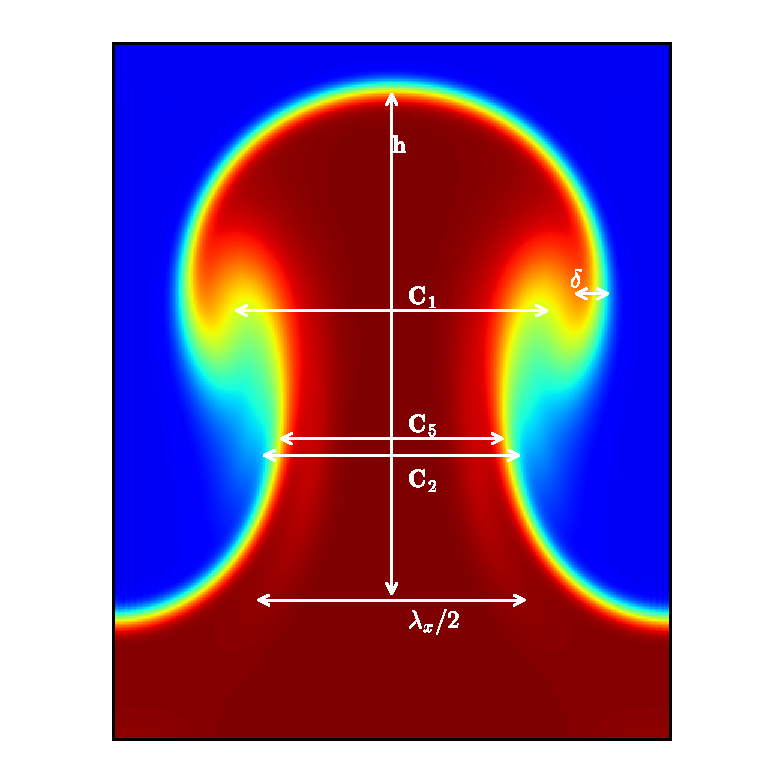
\includegraphics[width=\textwidth]{figs/slice}
\caption{Scalar $\phi$}
\end{subfigure}
\begin{subfigure}[b]{0.5\textwidth}
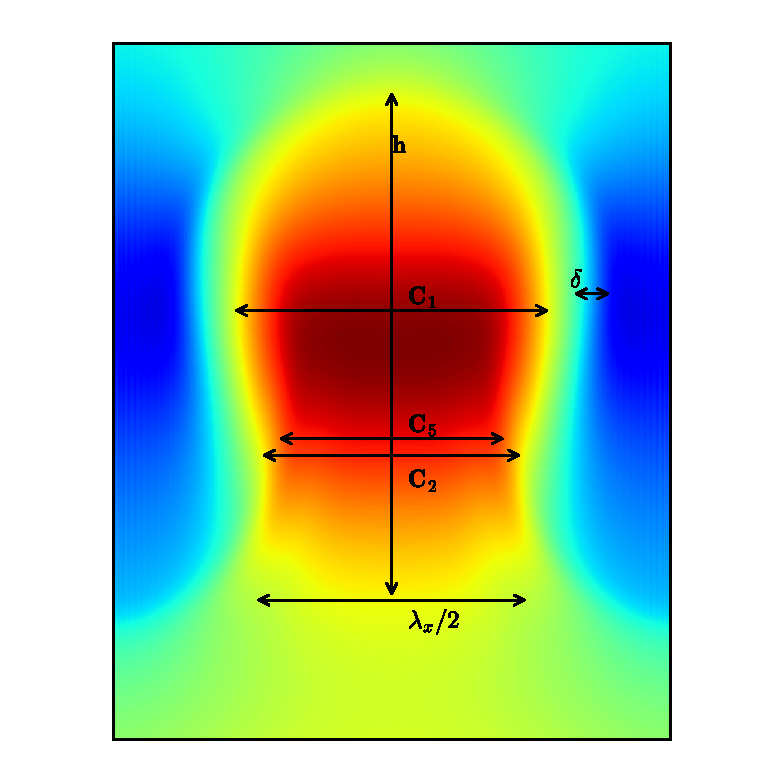
\includegraphics[width=\textwidth]{figs/slice_w}
\caption{Vertical component of the velocity, $w$}
\end{subfigure}
\caption{ \flabel{bubble_geom}
Slices of the scalar and vertical component of the velocity at early times and high Grashof number.
The arrows indicate the dependence of the model terms on different span-wise length scales, and are identical in both figures.
$C_1$ is related to the maximum cross sectional diameter of the bubble in the velocity field.
$C_2$ is related to the nominal side-wall diameter of the bubble in the velocity field.
$C_5$ is related to the nominal side-wall diameter of the bubble in the scalar field.
$\delta$ is related to the interface thickness in the scalar field.
The slice is in the plane $x=y$, which passes through only bubble centers.
}
\end{figure*}

The parameter $C_1$ scales the form drag and serves as a drag coefficient.  
Because we have let $C_0 = 1$, the force balance is really aggregated over two rising bubbles and two falling spikes, each with diameter $\lambda / 2$.
Therefore, we multiply the force on a single bubble of diameter $\lambda/2$ by 4.
Now, we relate $C_1$ to the drag coefficient $C_d$ in the drag equation:
\begin{equation}
	C_1 \lambda^2 \dot{h}^2 = 2 C_d \mathcal{A} \dot{h}^2,
\end{equation}
where $\mathcal{A}$ is the cross sectional area,
so $C_1$ can be estimated using drag coefficients of similar objects:
\begin{equation} \elabel{prior_c1}
C_1 = 2 C_d \frac{
	\mathcal{A}}{\lambda^2},
\end{equation}
where $\mathcal{A} \approx (\lambda/2)^2$.
Initially, the bubble tip is a flat plate, which has $C_d = 1.28$.
At late times, the bubble is closer to an elongated cylinder, which has $C_d = 0.82$, but with a somewhat streamlined tip, which further reduces drag.
We expect $C_1 \approx 0.64$, but possibly much smaller if the bubble takes a streamlined shape.
However, if the bubble spreads to have a diameter greater than $\lambda / 2$, $C_1$ could be greater than $0.64$.

Next, consider the limit when $h \rightarrow \infty$ and $D = 0$:
The dynamical equation becomes
\begin{equation}
\ddot{h} = \frac{A_0 g - C_2 \nu (1/\lambda) \dot{h}}{C_3},
\end{equation}
which leads to a terminal velocity of
\begin{equation} \elabel{visc_vel}
\dot{h} = \frac{A_0 g \lambda^2 }{C_2 \nu},
\end{equation}
or a non-dimensional velocity, i.e., Froude number,
\begin{equation}
\text{Fr} = \frac{d z}{d \tau} = \frac{\sqrt{\text{Gr}}}{C_2}.
\end{equation}
The case of extended bubbles and spikes affected only by viscous drag is highly analogous to flow through a square duct.
The pressure drop, $\Delta p$, along a duct is given by the Darcey-Weisbach formula:
\begin{equation}
\Delta p = \frac{f_D}{2} \frac{v^2 L}{d},
\end{equation}
where $L$ is the length of the duct,
$v$ is the mean velocity,
$d$ is the hydraulic diameter,
and $f_D$ is the Darcy friction factor.
In our case, $L = h$, $v = \dot{h}$, and $\Delta p = A_0 g h$, so
\begin{equation}
A g = \frac{f_D}{2} \frac{\dot{h}^2}{d}.
\end{equation}
For laminar flows in circular pipes, $f_D = \bar{f}_D = 64 / \text{Re}$, so
\begin{equation}
A g = \frac{f_D}{\bar{f}_D} 32 \nu \frac{\dot{h}}{d^2}.
\end{equation}
The hydraulic diameter $d = \lambda / 2$, so
\begin{equation}
\dot{h} = \frac{\bar{f}_D}{f_D} \frac{A_0 g \lambda^2}{128 \nu} .
\end{equation}
This gives an estimate for $C_2$:
\begin{equation}
C_2 \approx 128 \frac{f_D}{\bar{f}_D},
\end{equation}
where the ratio $f_D / \bar{f}_D$ is affected by the geometry and departure from laminar flow.
For example, for square ducts $f_D/\bar{f}_D \approx 0.889$, so $C_2 \approx 114$~\cite{ghiaasiaan2011convective}. 

The product of the coefficient $C_5$ and $\lambda h$ gives the interfacial area of the side of the bubble.
Therefore, $C_5$ captures information both about the bubble shape and the bubble diameter.
If the bubbles had diameter $\lambda / 2$ and were smooth and rectangular, then $C_5 \approx 4$.
If the bubble has a lower surface area shape, e.g., cylindrical, or is thinner, then $C_5 < 4$.

These diameters, along with the relevant span-wise length scales in the preceding coefficients, are sketched in \fref{bubble_geom}.
The diameter associated with $C_1$ is defined as the entrainment width at the bubble tip, in contrast to the width at the bubble center used for $C_2$.
The diameter associated with $C_5$ is defined similarly to $C_2$, but with respect to the scalar interface.
The interface width $\delta$ also depends on the scalar representation of the bubble.


\section{Numerical experiments} \slabel{exp}

To evaluate the simple model of \sref{model}, we conduct a battery of direct numerical simulations.
The novel components of the simple model, i.e. viscous drag and mixing, are most pronounced at late times.
We primarily direct our effort at simulating higher aspect ratio domains to allow the bubble to reach a dissipative flow.

The numerical experiments simulate the incompressible Navier-Stokes equations with the Boussinesq approximation:
\begin{align}
\frac{\partial u}{\partial t} + u \cdot \nabla u &= \nu \nabla^2 u - \nabla P + A g \phi \\
\frac{\partial \phi}{\partial t} + u \cdot \nabla \phi &= D \nabla^2 \phi 
\end{align}
where $u$ is the velocity,
$\nu$ is the kinematic viscosity,
$P$ is the pressure,
$\phi$ the non-dimensional density,
and $D$ is the diffusivity of $\phi$.

The initial conditions are quiescent with a horizontal interface perturbed by product of cosine functions and smeared by an error function:
\begin{equation}
\begin{split}
	\phi(x,y,z,t=0) = \\ 
	\text{erf}\left(\frac{z + a_0 \cos(2 \pi (x/\lambda)) \cos(2 \pi (y/\lambda))}{\delta})\right)
\end{split}
\end{equation}
where $a_0$ is the initial amplitude and $\delta$ is the initial interface thickness.
Both $a_0$ and $\delta$ are taken to be small enough to minimize their effects on the solution, $0.01$ and $1/128$, respectively.
The governing equations and initial condition have four dimensional parameters: $\nu$, $D$, $Ag$, $\lambda$.
These are combined into 2 non-dimensional numbers, the Grashof number and the Schmidt number:
\begin{equation}
\text{Gr} = \frac{A_0 g \lambda^3}{\nu^2} \quad \text{Sc} = \frac{\nu}{D}
\end{equation}
The Grashof number serves the role of a Reynolds number for instability problems without a consistent characteristic velocity.
For this reason, the root of the Grashof number is sometimes called the \textit{perturbation Reynolds number}~\cite{Wei2012}:
\begin{equation}
\text{Re}_p = \sqrt{\frac{A_0 g \lambda^3}{\nu^2}}
\end{equation}

The domain is $\left[0.5, 0.5, 64\right]$ and rotated 45 degrees in the span-wise plane to model $\lambda = \sqrt{2}$, transforming the initial condition to:
\begin{equation}
\begin{split}
	\phi(x,y,z,t=0) = \\
	\text{erf}\left(\frac{z + a_0 \cos(\pi (x+y)) \cos(\pi (x-y))}{\delta})\right).
\end{split}
\end{equation}
This is done so the span-wise boundaries at $x=\{0,0.5\}$ and $y=\{0,0.5\}$ are symmetric.
The length of the domain is $64/\sqrt{2} \approx 45.2$ wavelengths with no-slip walls at the top and bottom.
Based on a previous validation of the smRTI with no-slip boundaries, we expect the bubble to be unaffected by the top and bottom walls until it reaches 75\% of the height, or about $17\lambda$.
This provides significantly more data than the $h < 4 \lambda$ results of Ramaprabhu \etal~\cite{Ramaprabhu2012}.

The model introduced in \sref{model} assumes the bubbles and spikes are coherent structures, that is they travel at some velocity and have a well defined interface.
As the Grashof number increases and the bubbles and spikes break up, departing from the assumptions of the model.
On the other hand, at low Grashof number and finite diffusivity, diffusion moves the $\phi = 0$ interface, as opposed to simply transporting the scalar across it, which also departs from the model assumptions.
For these reasons, we restrict our study to an intermediate range of Grashof numbers: those which are large enough to sustain bubble dynamics while not being so large as to break the bubbles apart.
This range has been identified empirically to be approximately $6 \times 10^2 \le \text{Gr} \le 6 \times 10^5$ for Schmidt numbers greater than 1.

The number of spatial samples needed to resolve the advection-diffusion equation for the scalar goes with the Peclet number to the third power.
It is prohibitively expensive to perform calculations at high Schmidt numbers and high Grashof numbers.  

Simulations are performed with the NekBox version~\cite{NekBox} of the Nek5000 code~\cite{argonne:nekdoc}, which has been previously validated against single-mode Rayleigh-Taylor experiments~\cite{Hutchinson2016,Wilkinson2007}.
The spectral element method implemented by NekBox has purely dispersive errors and converges exponentially with the spectral order~\cite{Deville2002}.
The resolution parameters, the number of spectral elements, the order of the spectral elements, and the time step were chosen to achieve an accuracy of $10^{-4}$ in the bubble aspect ratio~\cite{hutchinson2016efficiency}.

\subsection{Observables}

\begin{comment}
\begin{figure}
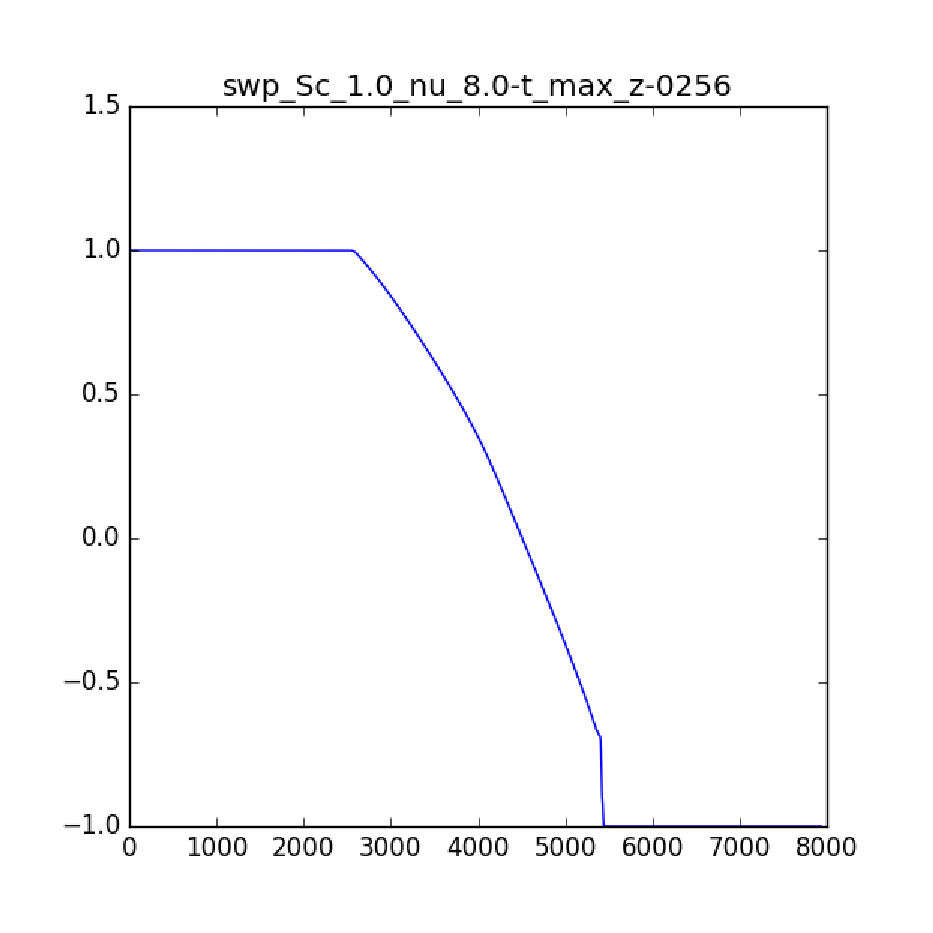
\includegraphics[width=\columnwidth]{figs/swp_Sc_1.0_nu_8.0-t_max_z-0256.eps}
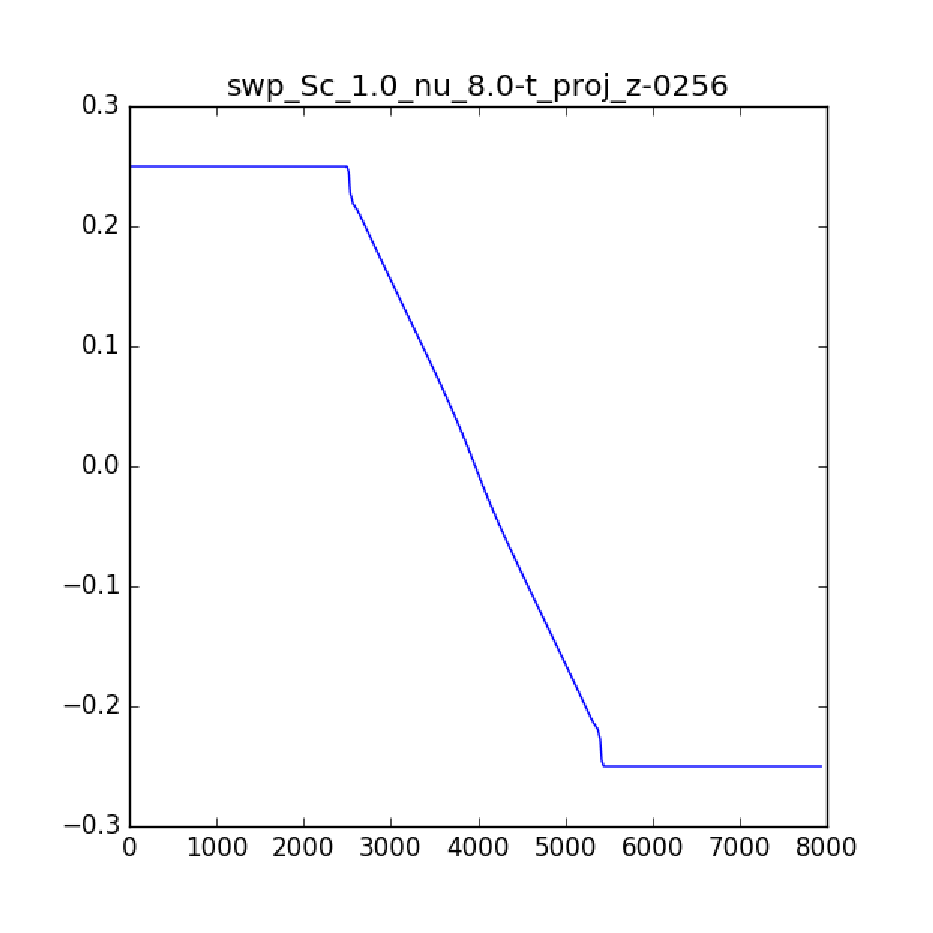
\includegraphics[width=\columnwidth]{figs/swp_Sc_1.0_nu_8.0-t_proj_z-0256.eps}
\caption{\flabel{profiles}
  Span-wise max and mean of scalar field.
}
\end{figure}
\end{comment}

\begin{figure}
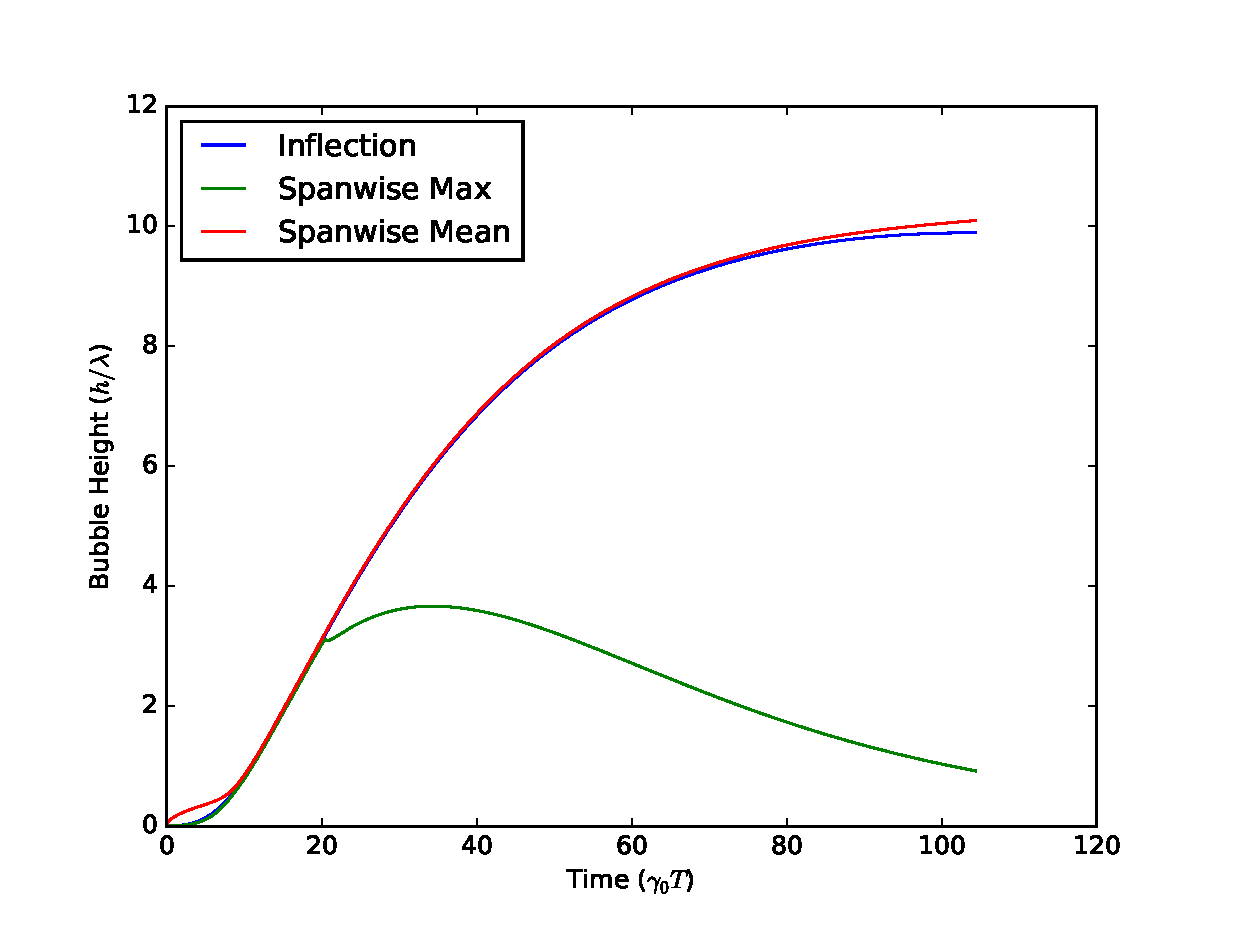
\includegraphics[width=\textwidth]{figs/comp-height-8-8}
\caption{ \flabel{heights}
  Comparison of height metrics at $\text{Gr} = 4.8\times10^4$ and $\text{Sc} = 1$.
}
\end{figure}


\paragraph{Bubble height}
For miscible RTI, the shape of the scalar field is due to a combination of advection in the bubble and diffusion across the interface.
We can assume an error function-like profile across the interface at the bubble tip, but diffusion across the bubble sidewalls results in a linear profile in both the span-wise mean and maximum of the scalar.
To separate the definition of the bubble tip from sidewall mixing, which is incorporated by the decreasing effective Atwood number, we introduce a new definition: the bubble tip is defined as the inflection point in the span-wise maximum scalar profile.
For the symmetric case, this span-wise maximum of the scalar is equivalent to the value along the bubble axis.
While mixing leads to a linear decay behind the bubble tip, the profile remains sharp near the bubble tip, decoupling the position of the inflection point from the sidewall mixing.

This definition of the bubble height is compared to two more traditional definitions, based on a cutoff in the mean or maximum profiles, in \fref{heights}.
At early times, the definition based on the mean profile grows diffusively.
At late times, the definition based on the max profile kinks as the linear part of the profile crosses zero and then stagnates.
The definition based on the inflection avoids both breakdowns while agreeing with the two traditional definitions within each of their valid ranges.

\paragraph{Mixed volume}

The scalar is normalized such that $\phi \in \left[-1, 1\right]$ and the average $\bar\phi = 0$.
The purity of the fluid is therefore $\left| \phi \right|$ and the volume of mixed fluid is given by a simple integral:
\begin{equation}
M(t) = \int \left( 1 - \left| \phi(x,y,z) \right|\right) dV
\end{equation}



\section{Growth stages through late times} \slabel{late}

\begin{figure*}
\begin{subfigure}[c]{0.5\textwidth}
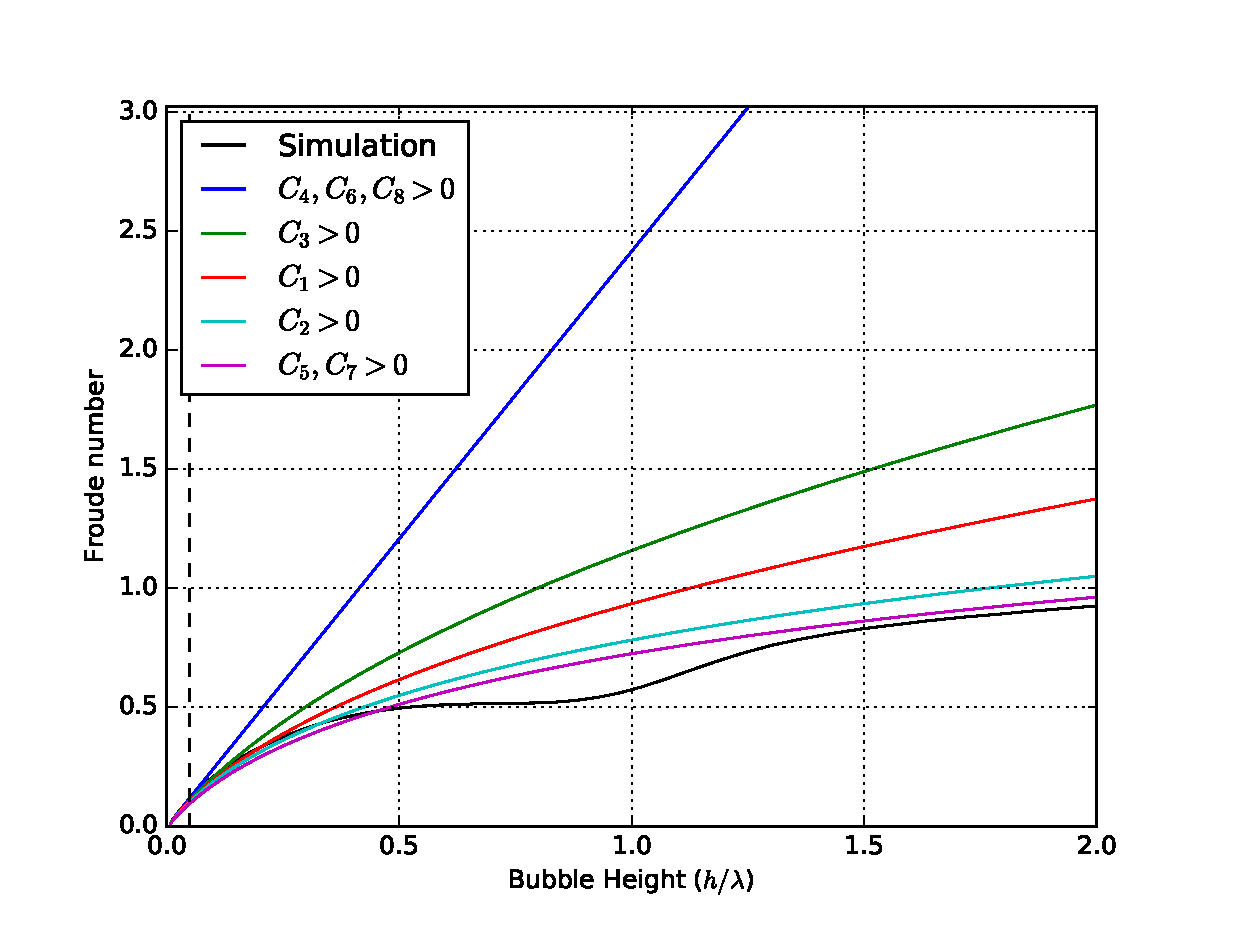
\includegraphics[width=\textwidth]{figs/Cascade-short-4-1}
\caption{Early times}
\end{subfigure}
\begin{subfigure}[c]{0.5\textwidth}
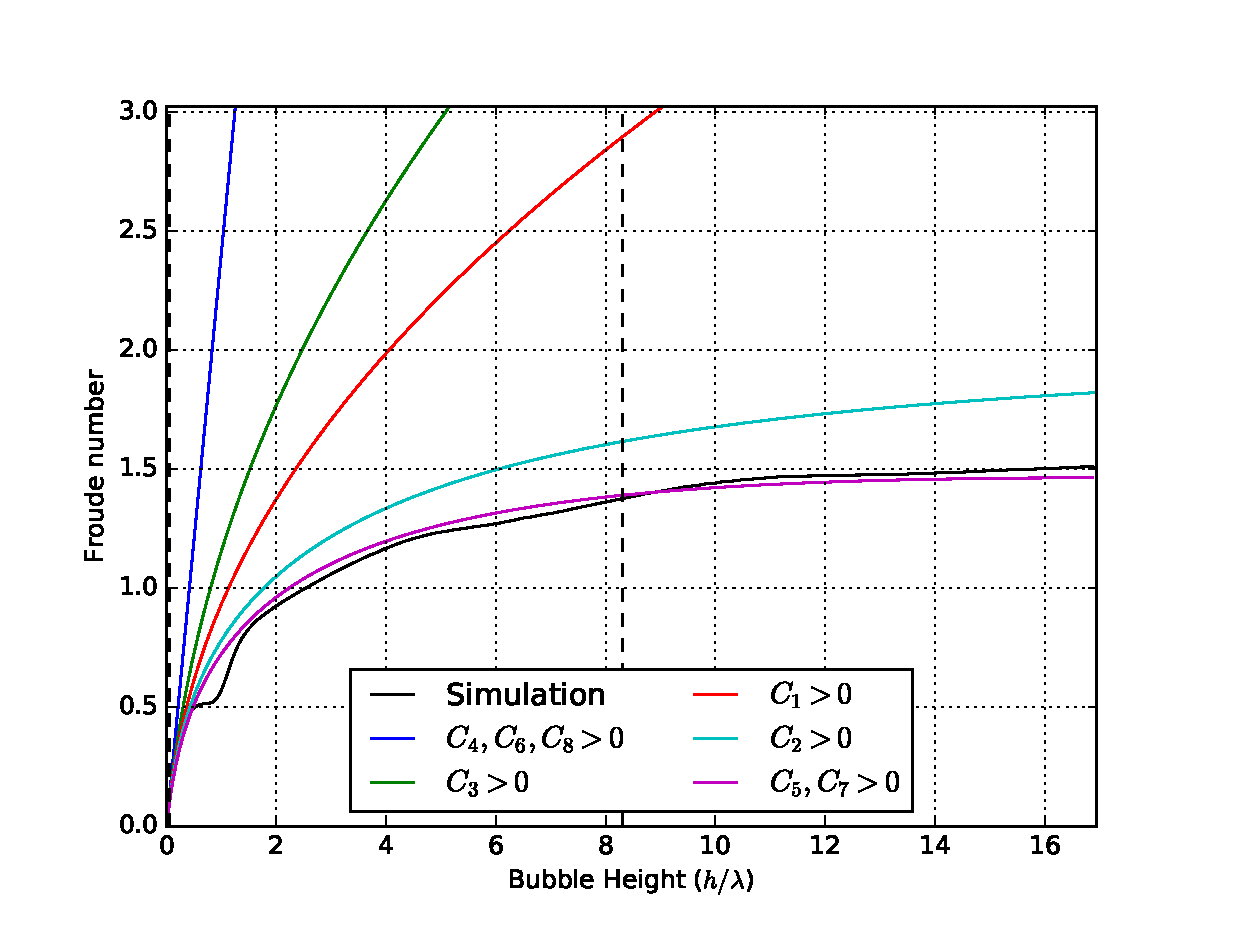
\includegraphics[width=\textwidth]{figs/Cascade-4-1}
\caption{Late times}
\end{subfigure}
\caption{ \flabel{high_Ra_traj}
Bubble Froude number vs non-dimensional bubble height for $\text{Ra} = 10^{5.75}, \text{Sc} = 4$, simulation vs model with successive terms enabled: first $C_4, C_6$ and $C_8$, then $C_3$, then $C_1$, then $C_2$, and finally $C_5$ and $C_7$.
The dashed vertical lines divide the trajectory into three regimes: linear growth for $H/\lambda < .05$, saturation until $H / \lambda \approx 8$, and viscosity beyond that.
The stagnation and re-acceleration transients are seen begining at $H/\lambda = 0.5$ and ending by $H / \lambda = 1.5$.
}
\end{figure*}

\begin{figure*}
\begin{subfigure}[b]{0.5\textwidth}
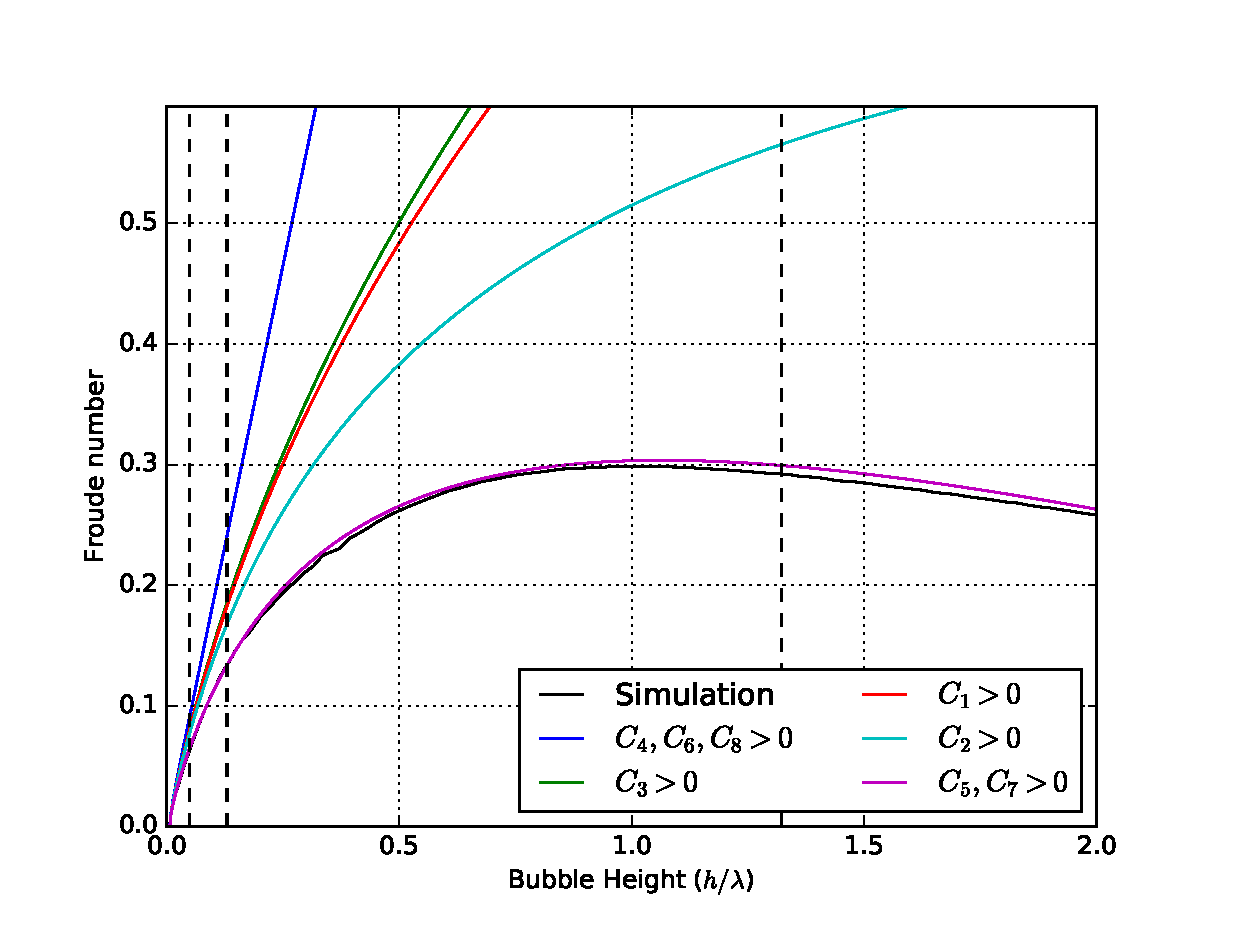
\includegraphics[width=\textwidth]{figs/Cascade-short-32-4}
\caption{Early times}
\end{subfigure}
\begin{subfigure}[b]{0.5\textwidth}
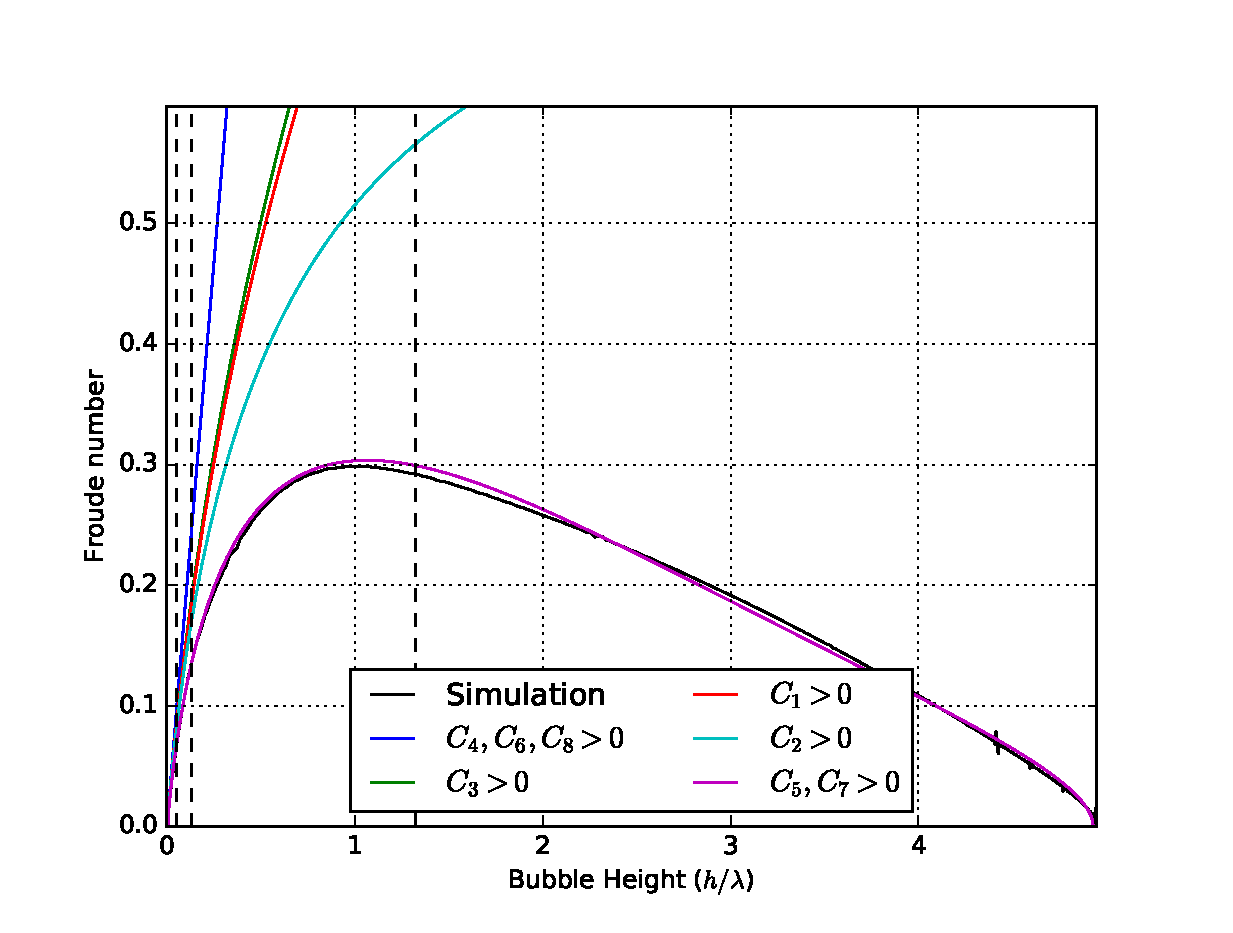
\includegraphics[width=\textwidth]{figs/Cascade-32-4}
\caption{Late times}
\end{subfigure}
\caption{ \flabel{low_Ra_traj}
Bubble Froude number vs non-dimensional bubble height for $\text{Ra} = 10^{4.5}, \text{Sc} = 8$, simulation vs model with successive terms enabled: first $C_4, C_6$ and $C_8$, then $C_3$, then $C_1$, then $C_2$, and finally $C_5$ and $C_7$.
Dashed vertical lines divide the trajectory into four regimes: linear growth for $H/\lambda < 0.05$, saturation until $H / \lambda \approx 0.1$, viscosity until $H / \lambda \approx 1.3$, and diffusion beyond that.
The stagnation and re-acceleration transients, seen in \fref{high_Ra_traj}, are suppressed by the viscous regime, which onsets before the transient begins at $H / \lambda = 0.5$.
}
\end{figure*}

Single mode experiments have been limited to bubble heights of $1.8\lambda$~\cite{Wilkinson2007}.
Simulations have reached in $4\lambda$ in 3D~\cite{Ramaprabhu2012} and $9\lambda$ in 2D~\cite{Wei2012}.
Here, we present trajectories that continue up to $17\lambda$, for example \fref{high_Ra_traj}.
However, the more dissipative bubbles stop rising at lower aspect rations, for example \fref{low_Ra_traj}.
Plotted with the non-dimensional bubble height, $h / \lambda$, and nondimensional mixed volume, $M / \lambda^3$ is the non-dimensional velocity, or Froude number, which is defined as:
\begin{equation}
  \text{Fr} = \frac{v}{\sqrt{A g \lambda}}
\end{equation}
The dissipation in the bubble is characterized by the Rayleigh number:
\begin{equation}
  \text{Ra} = \text{Gr} \text{Sc} = \frac{A_0 g \lambda^3}{\nu D}
\end{equation}

In the spirit of recent analyses~\cite{Ramaprabhu2012, Wei2012}, we try to identify distinct growth regimes.
To do so, we consider the behavior of the simple model with coefficients set to zero.
Initially, only $C_4$, $C_6$, and $C_8$ affect bubble dynamics.
The growth is exponential with a rate in agreement with the linear theory, so we term this the linear regime.
As the bubble grows, the $C_3$ term reduces the growth rate to a limiting value of $A g / C_3$.
Because this represents the transition from exponential growth to free-fall, we term it the saturation regime.
The $C_1$ term has the same qualitative effect as the $C_3$ term, so it doesn't distinguish a unique regime.
The $C_2$ term does impose a limiting velocity scale, so it departs significantly from the $C_3$ dynamics in the viscous regime.
Finally, the $C_5$ term, balanced by the $C_7$ term, mix the fluid and reduce the effective Atwood number in the diffusive regime.
Because the relative onset of the viscous and diffusive regimes depends on the Schmidt number, they are grouped together into the dissipative regime.
Ultimately, the bubble stops rising.
The bubble height at this point, which is also the maximum bubble height, is called the penetration depth.

\subsection{Exponential growth}
When the amplitude is small and the interface is thin, the linear theory and numerical results identify exponential growth: $\ddot{h} = \gamma^2 h$.
Similarly, in the limit $h, \delta \rightarrow 0$, the simple model yields a growth rate:
\begin{equation}
\gamma = \sqrt{\frac{A_0 g k}{2 \pi C_4(1 + C_8 / C_6 \pi^{1/2} k \delta)}},
\end{equation}
which differs from the linear theory by the absence of a $-D k^2$ term.
This is the only term that can cause unstable interfaces to decay, i.e. $\gamma < 0$ for positive Atwood numbers.
In the simple model, all unmixed bubbles grow while in the linear theory highly diffusive bubbles decay.

The other terms, \ie those scaled by $C_1, C_2, C_3, C_5$ and $C_7$, can be omitted while the description of the exponential growth is unaffected.

\subsection{Saturation regime}
The exponential growth saturates as the bubble height increases.
In the simple model, this captured by the $C_3$ term:
\begin{equation}
\ddot{h} = \frac{A g}{(C_3 h + C_4 \lambda) (1 + C_8 / C_6 \pi^{1/2} k \delta)},
\end{equation}
which becomes significant when $h \approx C_4 \lambda / C_3$.
We will find in the following section that $C_3$ takes a value of about 1, so, omitting viscous corrections, saturation halves the growth rate at $h \approx \lambda / (2\pi)$.

The definition of the start of the saturation regime is somewhat arbitrary.
Here, we propose the definition $h/\lambda < 0.05$ as it is where the exponential and saturated plots of the Froude number versus height visually deviate.
The important thing is that this threshold is independent of $Ag$, the Grashof number, and the Rayleigh number.
Within the saturation regime, the acceleration takes a limiting value of $Ag$, defining a saturation velocity:
\begin{equation} \elabel{vel_sat}
v_s \sim \sqrt{A g h}
\end{equation}

\subsection{Viscous regime}
As the bubble grows, so does its surface area.
The viscous drag, which scales linearly with the bubble height and bubble velocity, ultimately balances the buoyancy to limit the velocity, as in \eref{visc_vel}.
The scaling of the onset of this regime can be found by equating the saturation velocity and the viscous velocity:
\begin{equation}
\sqrt{A g h} \sim \frac{A g \lambda^2}{\nu}.
\end{equation}
Solving for $h/\lambda$ yields:
\begin{equation}
\frac{h_\nu}{\lambda} \sim \frac{A g \lambda^3}{\nu^2} = \text{Gr},
\end{equation}
where $h_\nu$ is the onset of the viscous regime.

As in the saturation case, the particular definition of the onset is arbitrary.
Here, we will define $h_\nu$ such that when $h_\nu/\lambda = 0.5$, the viscous velocity has the potential flow value: $v_\nu = \pi^{-1/2} \sqrt{A g \lambda}$.
This works out to be:
\begin{equation} \elabel{visc_height}
\frac{h_\nu}{\lambda} = \frac{\pi}{4 C_2^2} \text{Gr} \approx 4.7 \times 10^{-5} \text{Gr},
\end{equation}
where we've let $C_2 = 128$, the nominal value from Poiseuille flow.

\subsection{Diffusive regime}
\begin{figure}
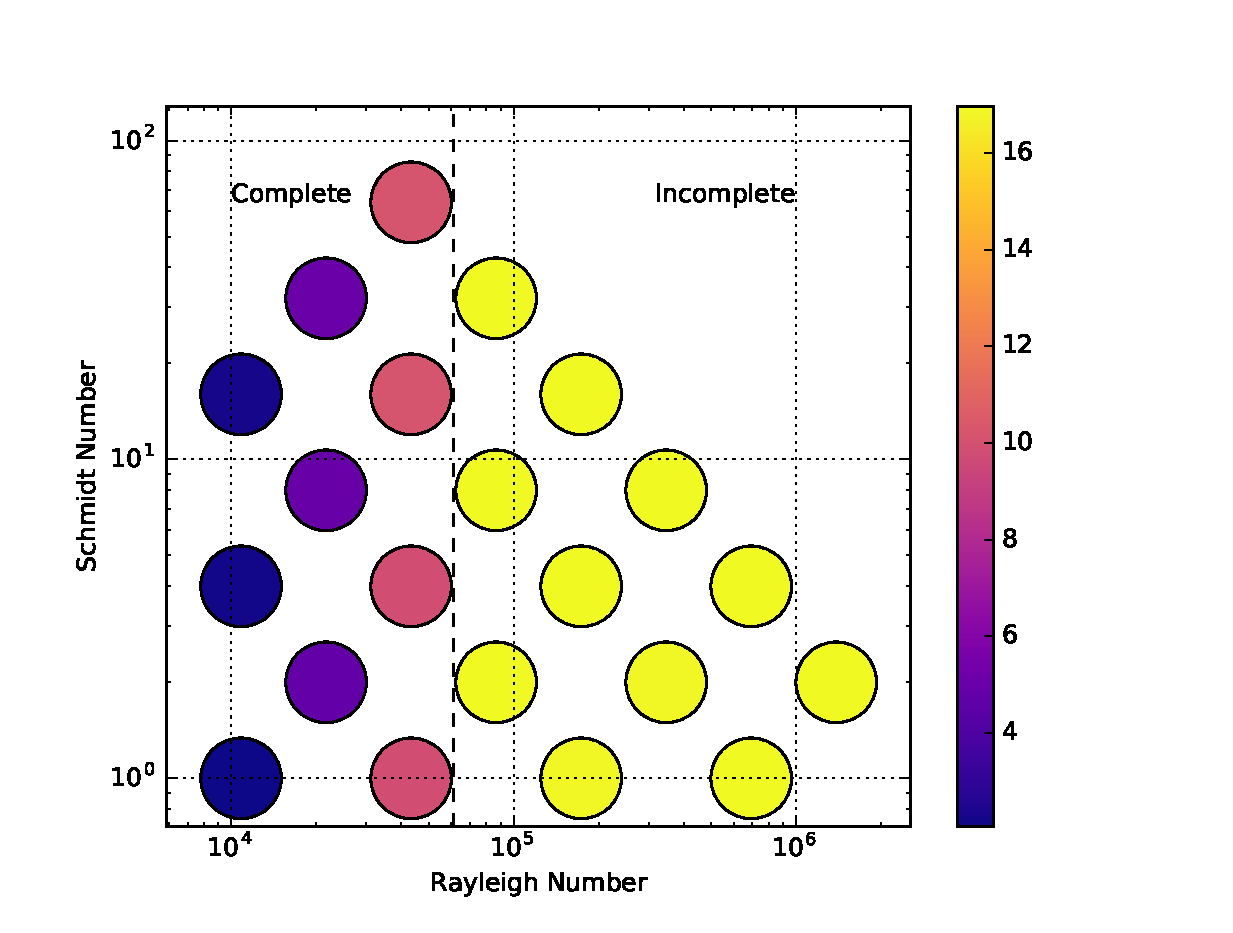
\includegraphics[width=\columnwidth]{figs/PenetrationDepth-vs-Rayleigh-Schmidt}
\caption{ \flabel{depth_scatter}
  Penetration depth, non-dimensionalized, vs the Rayleigh and Schmidt numbers.
  The dashed line separates completed from incomplete trajectories, which are clipped at $h/\lambda \approx 23$.
}
\end{figure}

\begin{figure}
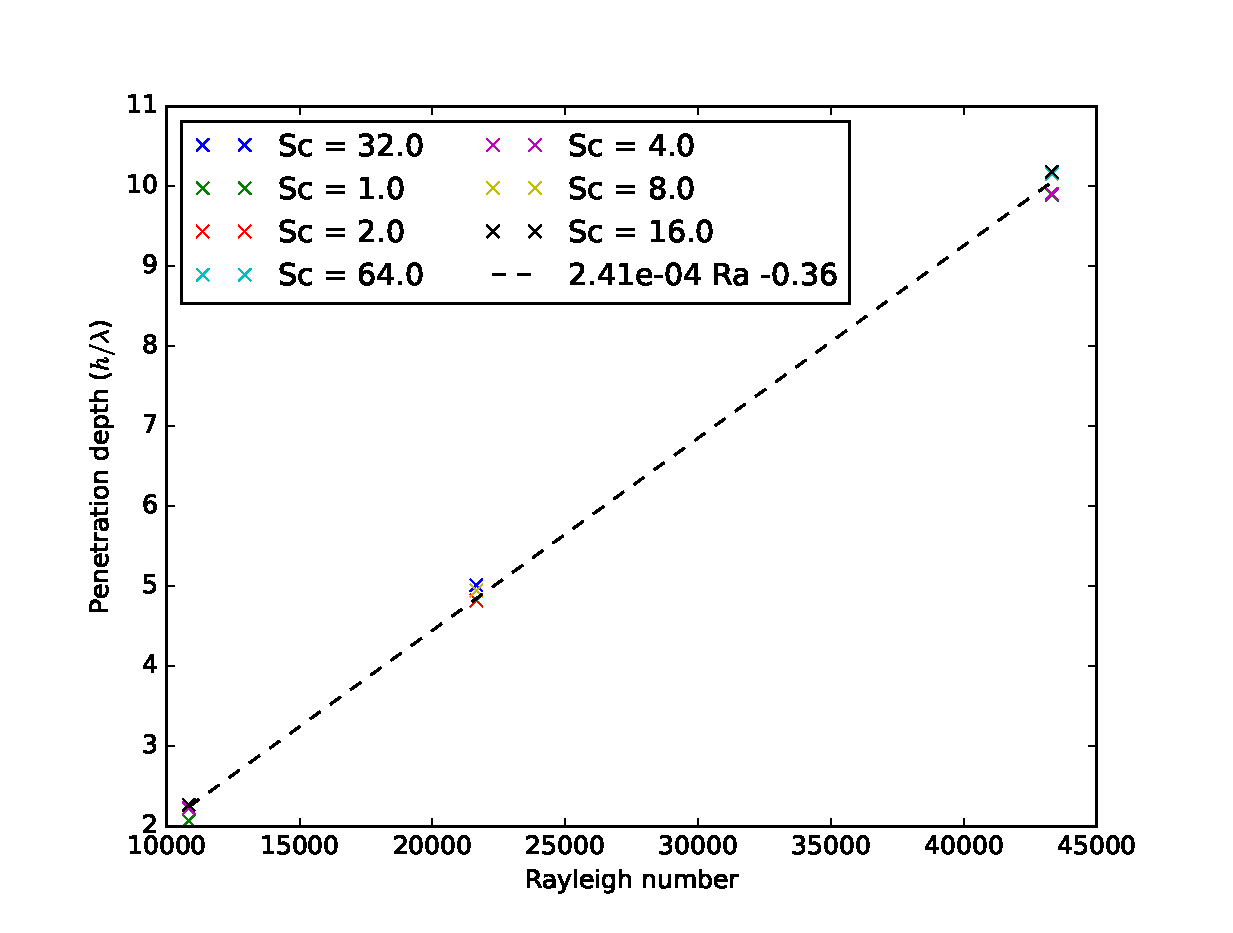
\includegraphics[width=\columnwidth]{figs/Depth-vs-Rayleigh}
\caption{ \flabel{depth_line}
  Penetration depth, non-dimensionalized, vs the Rayleigh.
  The dashed line is a best fit line $h/\lambda = 2.41 \times 10^{-4} \text{Ra} - 0.36$.
}
\end{figure}

The rate of diffusion across the surface of the bubble also scales with the bubble height.
When the viscous drag limits the bubble's velocity, the flux of pure fluid into the bubble, which goes as the velocity, is unable to match the flux of mixed fluid through the interface.
Mixing dilutes the buoyant fluid, reducing the Atwood number and therefore the bubble velocity.
Ultimately, the Atwood number reaches zero and eventually the bubble stops rising.

The penetration depth is the maximum height of the bubble, which is the height of the bubble at the stopping condition of this analysis.
We can estimate the scaling of the penetration depth as the product of a characteristic velocity with a characteristic time-scale.
The late-time velocity is the viscous velocity, $v_\nu$, while time-scale is given by diffusion:
\begin{equation}
\tau_D = \frac{\lambda^2}{D}.
\end{equation}
Combining and non-dimensionalizing yields:
\begin{equation}
\frac{h(\infty)}{\lambda} = \frac{A g \lambda^3}{\nu D} = \text{Ra},
\end{equation}
so the penetration depth should go linearly with the Rayleigh number.

The penetration depth is plotted as a function of Rayleigh and Schmidt number in \fref{depth_scatter}, and, indeed, depends strongly on the Rayleigh number before being clipped by the top walls.
Furthermore, the relationship to the Rayleigh number is linear over the cases shown here, as shown in \fref{depth_line}.

We can use a similar analysis to define the onset of the diffusive regime when the interface width is a quarter wavelength, $\delta = \lambda / 8$, which is a quarter of the nominal bubble diameter.
This results in a bubble height:
\begin{equation} \elabel{diff_height}
\frac{h_D}{\lambda} = \frac{1}{128 C_2} \text{Ra} \approx 6.1 \times 10^{-5} \text{Ra},
\end{equation}
where we've again let $C_2 = 128$.

The ratio of the diffusive to viscous heights, \eref{diff_height} and \eref{visc_height}, respectively, is linear with the Schmidt number, or about $1.3 \text{Sc}$.
For $\text{Sc} > 1$, the portion of the trajectory that is governed by viscosity alone increases with the Schmidt number.
However, for $\text{Sc} < 1$ the diffusive regime dominates the viscous regime entirely.

\subsection{Stagnation and re-acceleration}

Absent from the previous discussion is the stagnation and re-acceleration of the bubble around $h / \lambda = 1$, as seen in \fref{high_Ra_traj}.
There are no terms in the buoyancy-drag model capable of producing an inflection point in the Froude number vs bubble height, so stagnation and re-acceleration cannot be controlled by turning a model coefficient on or off.
This suggests that the buoyancy-drag model is missing a term.

However, the buoyancy-drag model does have a limiting velocity, the viscous velocity $v_\nu$.
When the viscous velocity is near or below the stagnation velocity, $\text{Fr} \approx \pi^{-1/2}$, saturation and re-acceleration are suppressed.
Otherwise, stagnation and re-acceleration temporarily interrupt the saturation regime.
The stagnation and re-acceleration is a transient regime that only occurs at sufficiently high Grashof numbers.



\section{Model fit coefficients} \slabel{fit}
\begin{table*}
\setlength{\tabcolsep}{12pt}
\centering
\pgfplotstabletypeset[
  col sep=space,
  columns/Gr/.style={sci,sci 10e,precision=1},
  columns/Ra/.style={sci,sci 10e,precision=1},
  columns/Sc/.style={column type/.add={}{|}},
%every first column/.style={
%column type/.add={|}{}
%},
%every last column/.style={
%column type/.add={}{|}
%},
  columns/$C_1$/.style={fixed,zerofill,precision=2},
  columns/$C_2$/.style={fixed,zerofill,precision=1,dec sep align},
  columns/$C_3$/.style={fixed,zerofill,precision=2},
  columns/$C_7$/.style={fixed,zerofill,precision=2},
  columns/$C_5$/.style={fixed,zerofill,precision=2, column type/.add={}{|}},
  columns/$E_d$/.style={
        column type=r,
        dec sep align,
        preproc/expr={100*##1},
        postproc cell content/.append code={
            \ifnum1=\pgfplotstablepartno
                \pgfkeysalso{@cell content/.add={}{\%}}%
            \fi
        },
        fixed,
        fixed zerofill,
  },
  columns/$E_m$/.style={
        column type=r,
        dec sep align,
        preproc/expr={100*##1},
        postproc cell content/.append code={
            \ifnum1=\pgfplotstablepartno
                \pgfkeysalso{@cell content/.add={}{\%}}%
            \fi
        },
        fixed,
        fixed zerofill,
  },
  every head row/.style={
        before row=\toprule,after row=\midrule},
  every row no 1/.style={after row=\midrule},
  every row no 4/.style={after row=\midrule},
  every row no 8/.style={after row=\midrule},
  every row no 13/.style={after row=\midrule},
  every row no 17/.style={after row=\midrule},
  every last row/.style={
        after row=\bottomrule},
]{tbl/coef.dat}
\caption{ 
Simulation conditions, fit coefficients, and relative errors. 
}
\end{table*}

\subsection{Fitting}

\begin{figure}
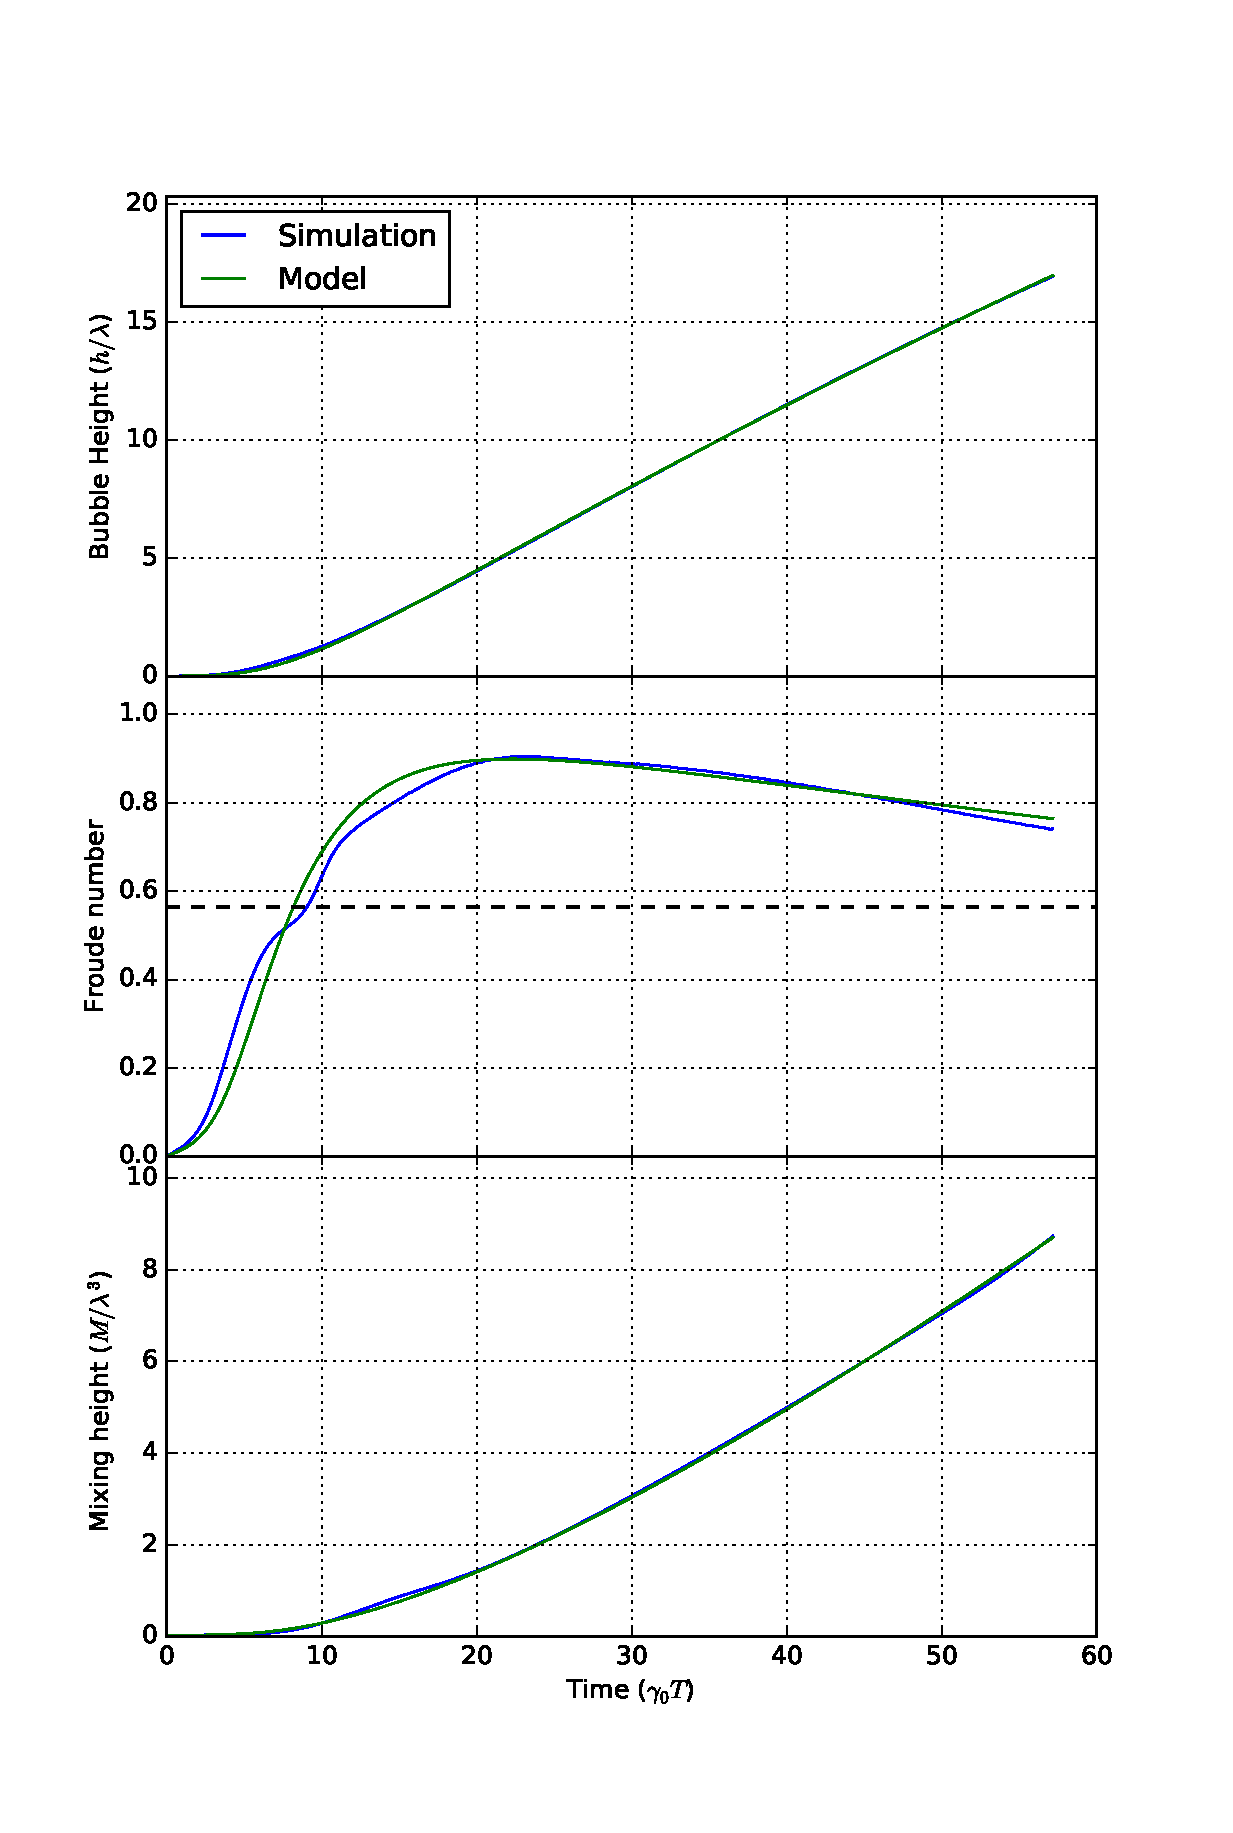
\includegraphics[height=\textheight]{figs/H-8-1}
\caption{ \flabel{example_fit}
  Example fit of the bubble height, top, and mixed volume, bottom, at $\text{Ra} = $ and $\text{Sc} = 8$.
  The dashed line is center plot is the stagnation velocity from potential flow models.
  The Froude number, which is a non-dimensional velocity, is not directly fit but shows agreement between the model and simulation.
}
\end{figure}

The mixing model defines the quantity of mixed fluid, $m(t)$, as an analytic function:
\begin{equation}
\left\{H(t), \delta(0), \lambda, D, C_5\right\} \rightarrow m(t),
\end{equation}
where $H(t)$ is the bubble height, 
$\delta(0)$ is the initial interface thickness,
$\lambda$ is the wavelength,
$D$ is the diffusivity, and 
$C_5$ is a mixing coefficient.
The values of $H(t)$, $\delta(0)$, $\lambda$, and $D$ are taken from the numerical experiments, allowing for the definition of an mixing error:
\begin{equation}
E_m = \left|\left|m\left[C_5\right] - M(t) \right| \right|_2,
\end{equation}
where $M(t)$ is the reference value from the numerical experiments.
To compute $C_5$, the error is minimized under the constraint $C_5 > 0$.
The fitting problem is non-linear but 1D dimensional, so it can be solved with a sequential least squares minimizer, which finds local minima, wrapped with a basin hopping scheme, which samples across the local minima.

The dynamics model defines the bubble height, $h(t)$, as the solution to an ordinary differential equation.
The dynamics model is integrated using the variable-coefficient ordinary differential equation (VODE) solver for stiff systems, creating a map from the dynamics coefficients to the height:
\begin{equation}
\left\{h(0), \delta(0), \lambda, \nu, D, C\right\} \rightarrow h(t),
\end{equation}
where $h(0)$ is the initial bubble height,
$\delta(0)$ is the initial interface thickness,
$\lambda$ is the wavelength,
$\nu$ is the kinematic viscosity,
$D$ is the diffusivity, and
$C$ are the model coefficients.
$\delta(0)$, $\lambda$, $\nu$, and $D$ are taken from the simulation while $C_5$ is taken from independently fitting the mixing model, allowing for the definition of a dynamics error:
\begin{equation}
E_d = \left| \left| h\left[C_1, C_2, C_3, C_7\right] - H(t)\right| \right|_2,
\end{equation}
where $H(t)$ is the reference value from the numerical experiments.
The non-linear global minimization problem is solved with the covariance matrix adaptation evolution strategy (CMA-ES).
CMA-ES iteratively refines a sample distribution that evolves towards the global optimum.
Computing the model error is very inexpensive compared to the simulations, so we choose a broad initial distribution with a large population size.
The stochastic solution is polished with a sequential least-squares local minimization.

However, the high Rayleigh trajectories are incomplete, in that the data ends when the bubble gets close to the top wall, leading to under-constrained systems.
Therefore, we regularize the fit by adding a term to the model error:
\begin{equation}
R = \beta \left| \left| \frac{C - \bar{C}}{\bar{C}} \right| \right|_2,
\end{equation}
where $\beta$ is the regularization parameter,
$C$ is the vector of model coefficients, and
$\bar{C}$ are the coefficient estimates.
Although the buoyancy-drag model is non-linear, this L2 regularization can be thought of as a Tikhonov regularization~\cite{roths2001generalized} or ridge regression~\cite{marquardt1975ridge}.
The regularization parameter is chosen to be an order smaller than the model error, $\beta = 0.1 E_d$.
The if the regularized dynamic error ends up lower than the unregularized error, the unregularized problem must not have converged to the local minima.
In those cases, the unregularized fit is repeated with the regularized coefficient values as a starting seed.
Then the regularized fit is repeated with the updated definition.
In this way, the two types of fits are iterated until consistency is reached.

The fitting process defines a mapping from the Grashof and Schmidt numbers to the model coefficients and model errors:
\begin{equation}
\left(\text{Gr}, \text{Sc}\right) \rightarrow \left(C_1, C_2, C_3, C_5, C_7, E_m, E_d\right) 
\end{equation}
The rest of this section explores the relationships in this mapping.

\subsection{Scope of the models}

The proposed models aim to describe the mixing and dynamics in rising Rayleigh-Taylor bubbles and falling Rayleigh-Taylor spikes.
The symmetry of the governing equations equates the spike behavior to that of the bubbles, so we will omit spikes from the following discussions.
In highly viscous and diffusive cases, the bubbles may not reach late time highly non-linear dynamics.
For this analysis, a bubble is considered to be covered by the model only if its height exceeds its wavelength before it stops rising.
Experiments which do not meet that condition are discarded.

The bubble grows until mixing dilutes its buoyancy sufficiently for it to stop rising.
After this point, it slowly recedes due to diffusing across the bubble tip.
The model does not account for this diffusive effect, which moves move the center of the interface rather than just broadened it, so bubble trajectories are clipped beyond the point at which the bubble velocity is zero.
The height at that point in the trajectory is maximal and called the \textit{penetration depth}.

The penetration depth increases with Rayleigh number.
For high Rayleigh number cases, the bubble continues to grow until it beings to interact with the top boundary, given the finite computational domain.
Based on previous validation studies~\cite{Hutchinson2016}, we clip the trajectory when the bubble height reaches 75\% of the domain height.
Experiments in which this clipping occurs are incomplete.
Those cases should be re-simulated with a larger computational domain, at greater computational cost, to collect trajectories which reach their penetration depth.

However, there is still information in the incomplete experiments.
In the following sections, incomplete experiments will be marked as such, but the trend in the complete experiments is often seen to continue smoothly into incomplete ones.
Though not definitive, those suggest that the data present in the incomplete experiments is sufficient to constrain the corresponding characterization of the flow.
Conversely, in some cases the behavior in the incomplete experiments departs from that in the complete ones. 
In those cases, it is difficult to differentiate between Rayleigh-dependent behavior and the side-effects of underconstrained fitting.

It should be noted that the computational cost of a complete trajectory goes as $\text{Gr}^4 \text{Ra}^2 \max(1, \text{Sc}^4)$.
The fourth power of the Grashof and Schmidt numbers come from stability constraints: three from the spectral constraint and 1 from the explicit time-stepping constraint.
The square of the Rayleigh number comes from the penetration depth, which both increases the length of the domain and the number of time-steps taken.
For $\text{Sc} \ge 1$, the cost simplifies to $\text{Ra}^6$.
For the runs in this study, the cheapest incomplete trajectories will cost $64\times$ more than most expensive completed ones.
The most expensive incomplete trajectory, at $\text{Ra} \approx 1.4\times 10^6$, will cost over $10^9\times$ more than cheapest completed one.

\subsection{Accuracy of the models}

\begin{figure*}
\begin{subfigure}[b]{0.5\textwidth}
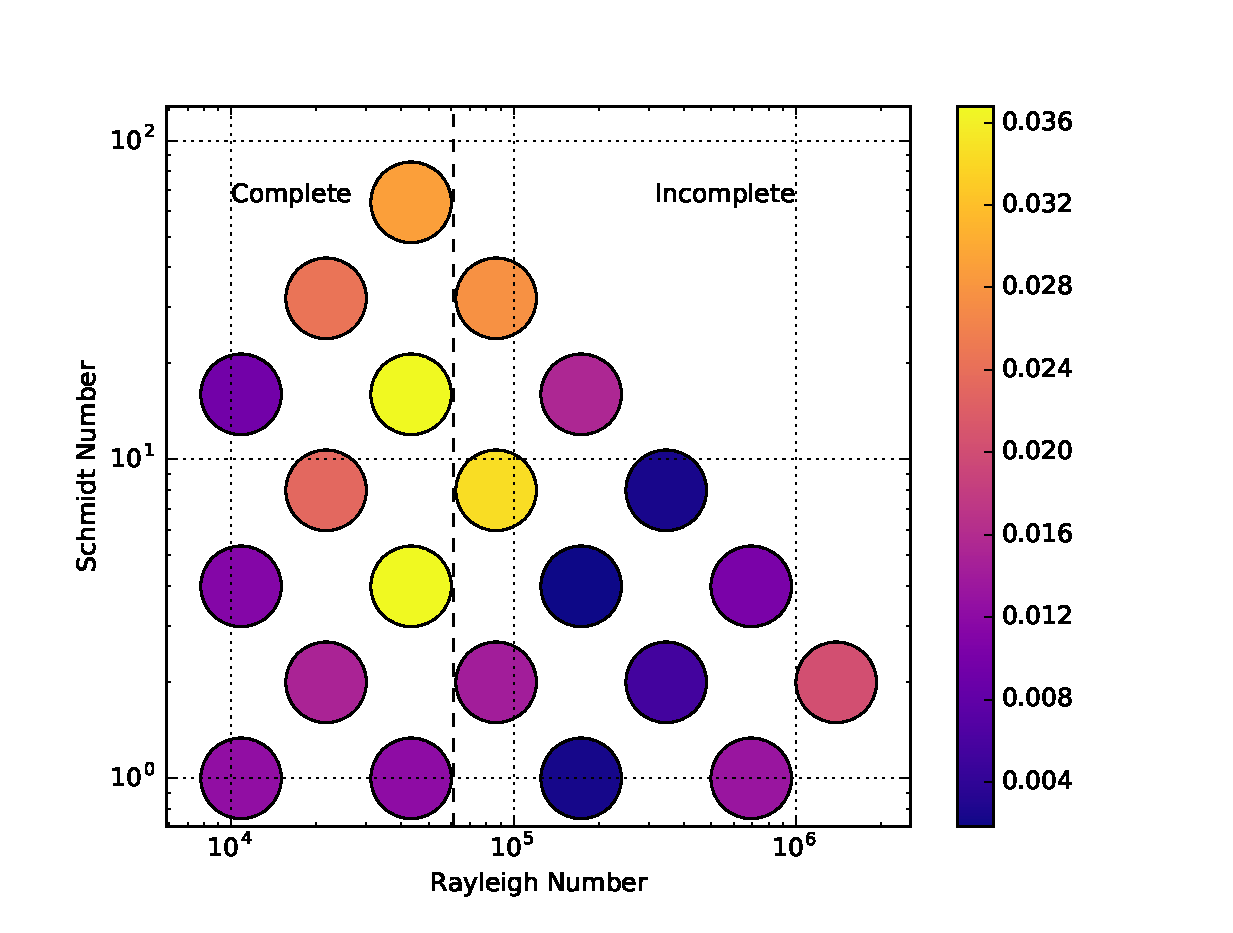
\includegraphics[width=\textwidth]{figs/MixingError-vs-Rayleigh-Schmidt}
\caption{Relative mixing error, $E_m/\text{max}[M(t)]$}
\end{subfigure}
\begin{subfigure}[b]{0.5\textwidth}
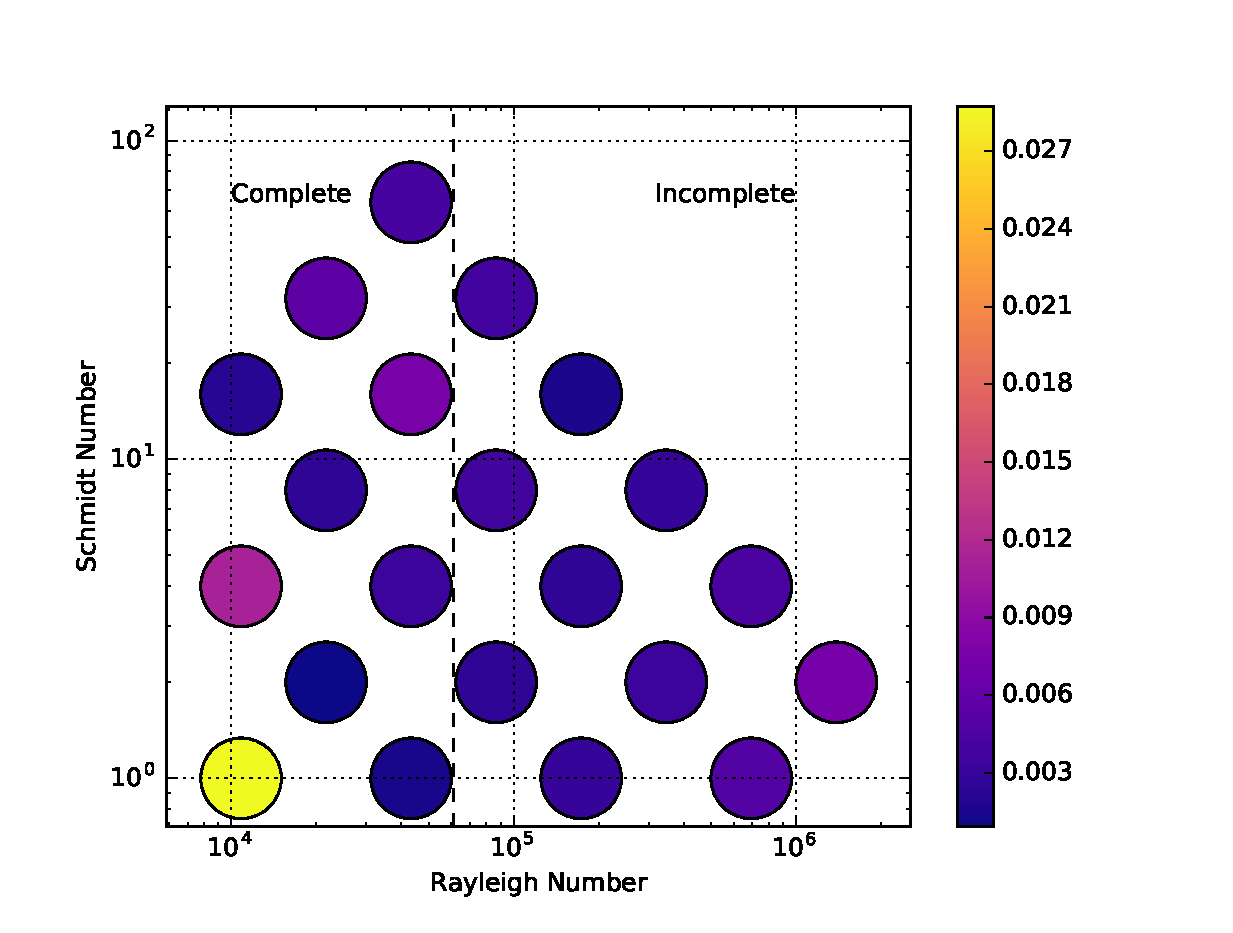
\includegraphics[width=\textwidth]{figs/DynamicsError-vs-Rayleigh-Schmidt}
\caption{Relative dynamics error, $E_d/\text{max}[H(t)]$}
\end{subfigure}
\caption{ \flabel{errVsParam}
  Relative model errors versus Rayleigh and Schmidt numbers.
  Experiments on the left side of the dashed line completed when the bubble stopped rising.
  Experiments on the right side of the dashed line are incomplete, having approached the vertical boundaries of the simulated domain.
}
\end{figure*}

The accuracy is characterized by the mixing and dynamics model errors relative to the maximum mix volume and bubble height, respectively.
The relative model errors are plotted versus the Rayleigh and Schmidt numbers in \fref{errVsParam}.
In both models, the nominal error is less than 5\%, but the two errors have differing structures.

The relative mixing error is about 3\% for the complete experiments, with generally greater relative error at greater Rayleigh and Schmidt numbers.
Among the incomplete experiments, relative error decreases with Rayleigh number before increasing again.
This is likely due to the incompleteness; the greater error above $\text{Ra} = 10^6$ suggests that the overall trend is increasing.
Overall, the relationship between the accuracy of the mixing model the Rayleigh and Schmidt numbers is incomplete.

The relative dynamics error is about 1\%, with the exception of the unit Schmidt $\text{Ra} \approx 10^4$ case.
The mixing error for the outlying case is typical, so the error cannot be attributed to the treatment of mixing.
This case will be considered more in the following sections.
Outliers aside, the relative error decreases with Schmidt number and Rayleigh number, both for complete and incomplete trajectories.
This indicates the dynamics model is most accurate, at least relative to the mixing height, when there is less mixing and drag.
Another factor is re-acceleration, which adds some relatively constant error that is amortized more when the penetration depth is greater.


\begin{comment}
The model proposed in \sref{model} assumes the bubble is a coherent structure with a single velocity.
If the Grashof number is high, then the bubble can break up into multiple smaller bubbles as the bubble accelerates.
The break-up is easily identified visually.
Increasing the Grashof number, Schmidt number, or both should enhance the break-up, so we can identify a bifurcation boundary for the break-up.

On the other hand, at low Grashof and Schmidt numbers, the growth of bubble height can be dominated by the growth of the interface width, leading to predominantly diffusive dynamics.
This is particularly evident when the bubble height recedes, a process which is not accounted for in the buoyancy-drag model.
When the bubble velocity reverses, the trajectory is truncated for the purposes of fitting.
We can identify cases for which the bubble height recedes over the first time unit.
Similar to the break-up, decreasing the Grashof number, Schmidt number, or both should suppress the bubble growth, so we can identify a bifurcation boundary here as well.
\end{comment}


\subsection{Fit coefficients}
The proposed model has 5 undetermined parameters.
In each case, we estimate the value a priori by physical arguments.
Then, the estimates are used as the starting point for fitting, that is minimization of the model error over the scope of the model.

\subsubsection{Form drag coefficient, $C_1$}

\begin{figure}
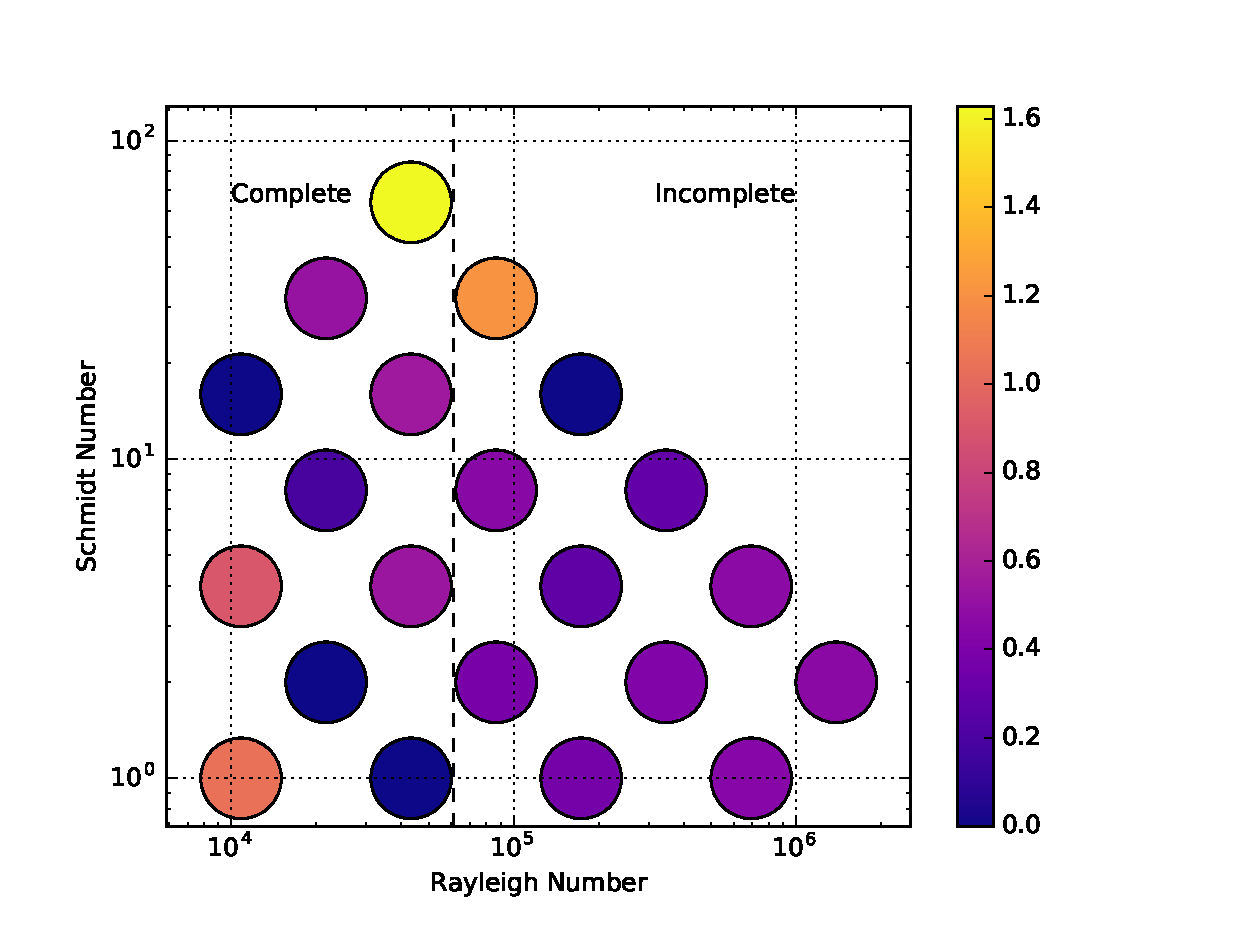
\includegraphics[width=\columnwidth]{figs/C1-vs-Rayleigh-Schmidt}
\caption{ \flabel{C1VsParam}
  Best fit for $C_1$ versus Rayleigh and Schmidt numbers.
  Experiments on the left side of the dashed line completed when the bubble stopped rising.
  Experiments on the right side of the dashed line are incomplete, having approached the vertical boundaries of the simulated domain.
}
\end{figure}

The coefficient $C_1$ is related to the drag coefficient $C_d$ by \eref{prior_c1}.
Therefore we expect it to take a value around or less than $0.64$, which corresponds to the drag coefficient of a flat plate and a surface area $A = \lambda^2$.

The $C_1$ term is most influential early in the flow, so we expect it to be well constrained even in the incomplete trajectories.
However, the $C_1$ term is qualitatively redundant with the $C_3$ inertial term, as they both bound the acceleration but not the velocity.
Similarly, viscous drag is weak but still present at early times.
It is possible that late-time effects that influence $C_2$ could have an indirect effect on the value of $C_1$.

The fit values of $C_1$ are plotted vsersus the Rayleigh and Schmidt numbers in \fref{C1VsParam}.
The majority of trajectories are closely grouped between $0.3$ and $0.6$, which fits the drag coefficient rationale.
However, there are outliers both at $C_1 = 0$ and $C_1 > 0.9$.
These outliers are troubling because each type occurs at both high and low Schmidt number and at low to moderate Rayleigh numbers.
There is no clear pattern, but there are no outliers at the high Rayleigh-number.

\subsubsection{Skin drag coefficient, $C_2$}
\begin{figure}
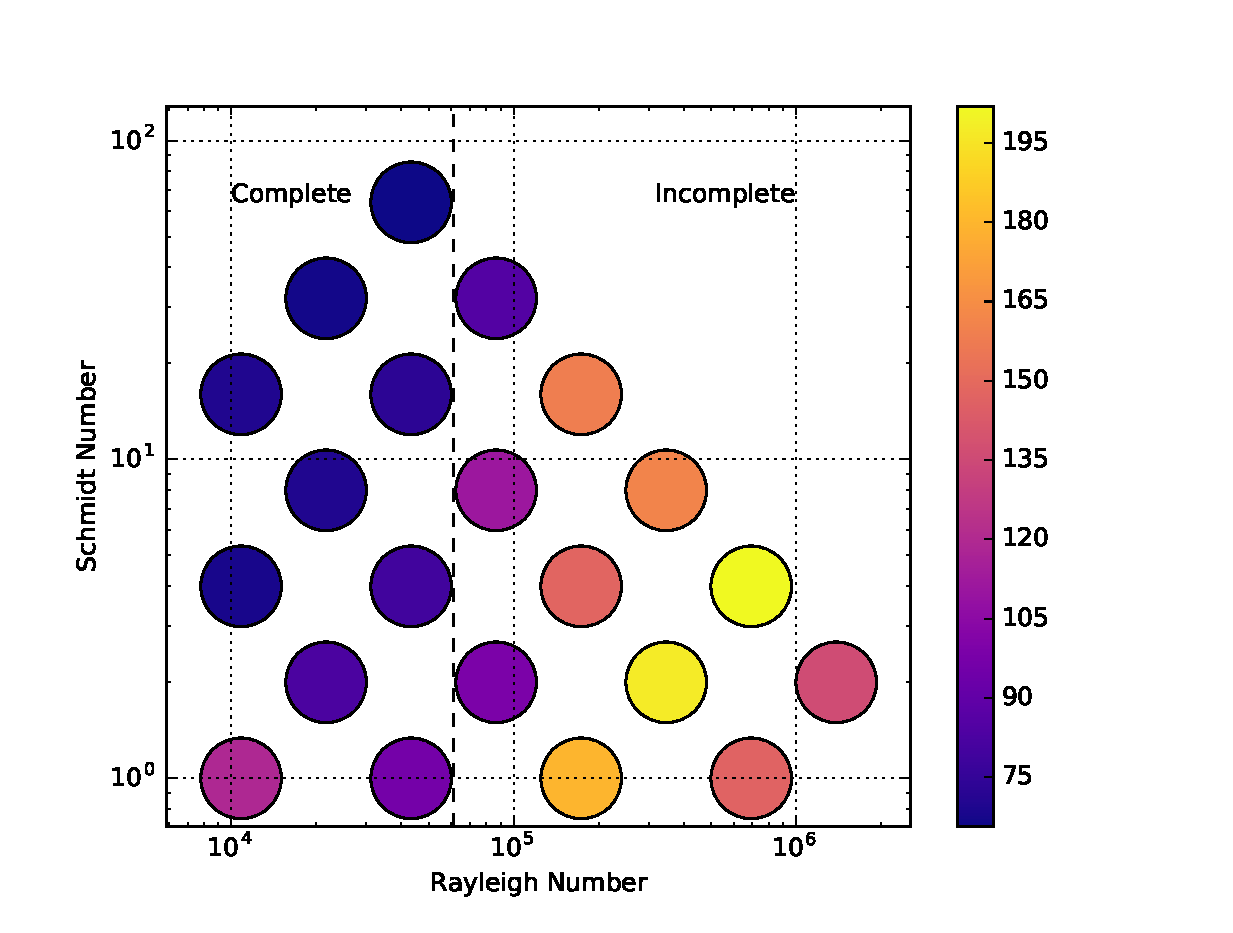
\includegraphics[width=\columnwidth]{figs/C2-vs-Rayleigh-Schmidt}
\caption{ \flabel{C2VsParam}
  Best fit for $C_2$ versus Rayleigh and Schmidt numbers.
  Experiments on the left side of the dashed line completed when the bubble stopped rising.
  Experiments on the right side of the dashed line are incomplete, having approached the vertical boundaries of the simulated domain.
}
\end{figure}

The coefficient $C_2$ scales the viscous drag.
As with $C_1$, $C_2$ can be related to a standard measure of drag, in this case the Darcy friction factor, which provides an estimate of 113.
The $C_2$ term is linear with $h$ and $\dot{h}$, so its influence is greatest at moderate to late times.
Therefore, values of $C_2$ taken from incomplete trajectories should be taken with a grain of salt.

The fit values of $C_2$ are plotted versus the Rayleigh and Schmidt numbers in \fref{C2VsParam}.
For the completed trajectories, $C_2$ is about $60$ and grows slightly with the Grashof number while being nearly independent of the diffusivity.
At higher Rayleigh numbers the incomplete trajectories also show $C_2$ growing with Grashof number, but the effect is much stronger.
There is weaker growth as the diffusivity decreases.
Finally, at the highest Grashof numbers the $C_2$ coefficient moderates again.

The presense of a positive relationship between $C_2$ and the Grashof number in both the complete and incomplete trajectories suggests it is a real effect, though its strength is unclear.
The relationship between $C_2$ and the diffusivity is much weaker and could disappear as the high Rayleigh trajectories are completed.

One possible mechanism for increasing $C_2$ with increasing Grashof number is the development of small amplitude Kelvin-Helmholtz structures on the bubble surface.
These structures are suppressed at low Grashof number and grow more rapidly at higher Grashof number.
They would enhance the transport of momentum across the bubble interface, thereby increasing the viscous drag coefficient.

\subsubsection{Inertial coefficient, $C_3$}
\begin{figure}
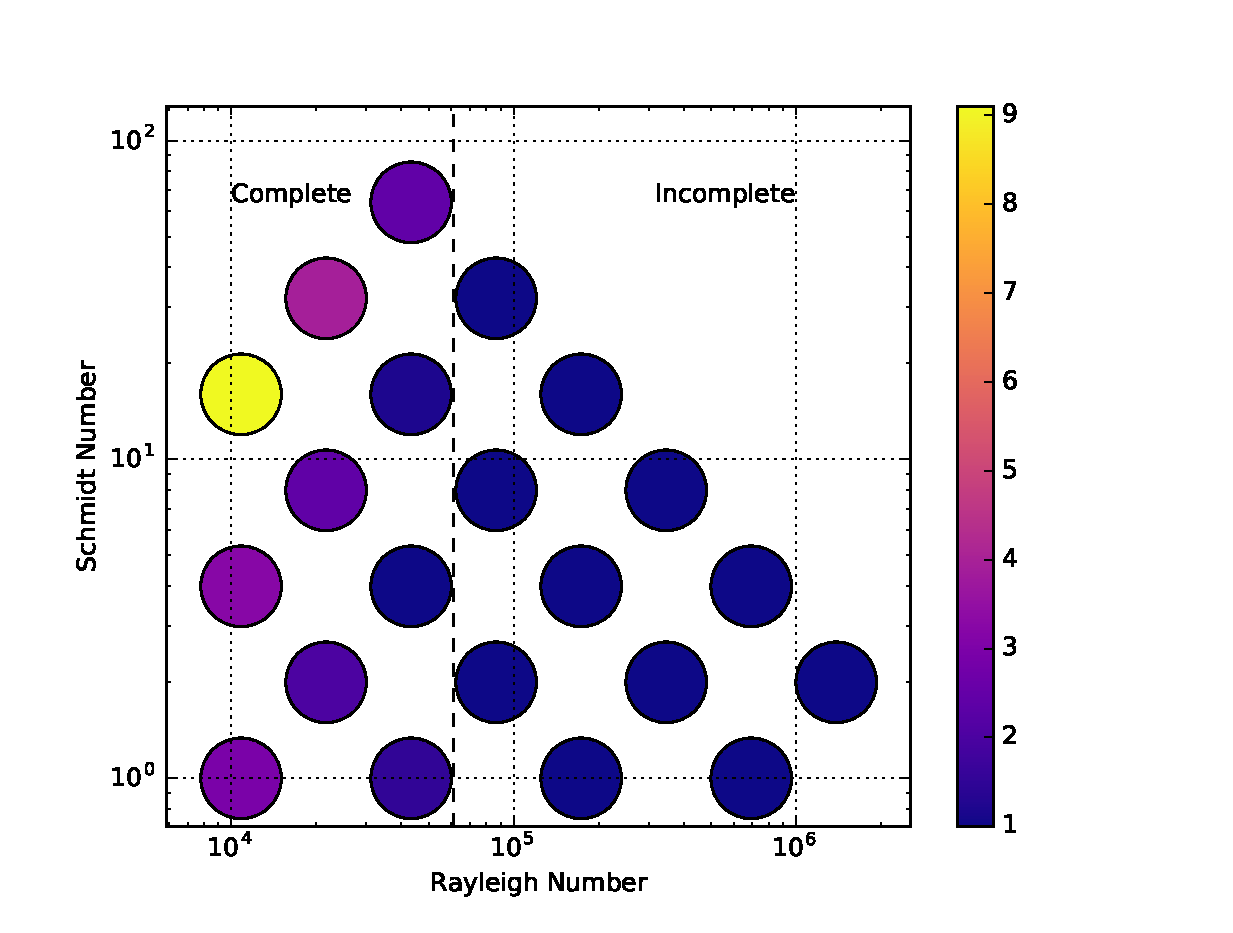
\includegraphics[width=\columnwidth]{figs/C3-vs-Rayleigh-Schmidt}
\caption{ \flabel{C3VsParam}
  Best fit for $C_3$ versus Rayleigh and Schmidt numbers.
  Experiments on the left side of the dashed line completed when the bubble stopped rising.
  Experiments on the right side of the dashed line are incomplete, having approached the vertical boundaries of the simulated domain.
}
\end{figure}

The coefficient $C_3$ gives the ratio of the inertial height to the buoyant height.
For $C_3 = 1$, the maximum bubble acceleration is $A g$ while $C_3 > 1$ represents the entrainment of neutrally or anti-buoyant fluid that contributes to the inertia but not the forcing.
Mixing, which also reduces the ratio of the forcing to the inertia, is accounted for explicitly with the $C_5$ coefficient and fit independently to the mixed volume observable, which prevents it from compensating for entrainment.
The $C_3$ term is linear with the height, so its influence is most pronounced at greater values of the height.

The fit values of $C_3$ are plotted versus the Rayleigh and Schmidt numbers in \fref{C3VsParam}.
The majority of trajectories have $C_3 = 1$, indicating that entrainment is not significant.
For completed low Rayleigh high Schmidt flows $C_3$ increases to a value of $9.1$.
However, the nominal value of $1$ is recovered within the completed trajectories.
Because the $C_3$ term depends on the height, it is relatively underconstrained at lower Rayleigh numbers.
If the model values of $C_4$, $C_6$, or $C_8$ are incorrect, the $C_3$ term has the greatest ability to compensate for the error when the height and velocity are small.
However, the height is still small, so $C_3$ would have to change significantly.
The author belives that $C_3 = 1$ is therefore the nominal value, but there is a breakdown in the model at low Rayleigh numbers that is influencing the fit of $C_3$.
Identifying and correcting this model breakdown would be expected to recover $C_3$ at low Rayleigh number.

\subsubsection{Interfacial area coefficient, $C_5$}
\begin{figure}
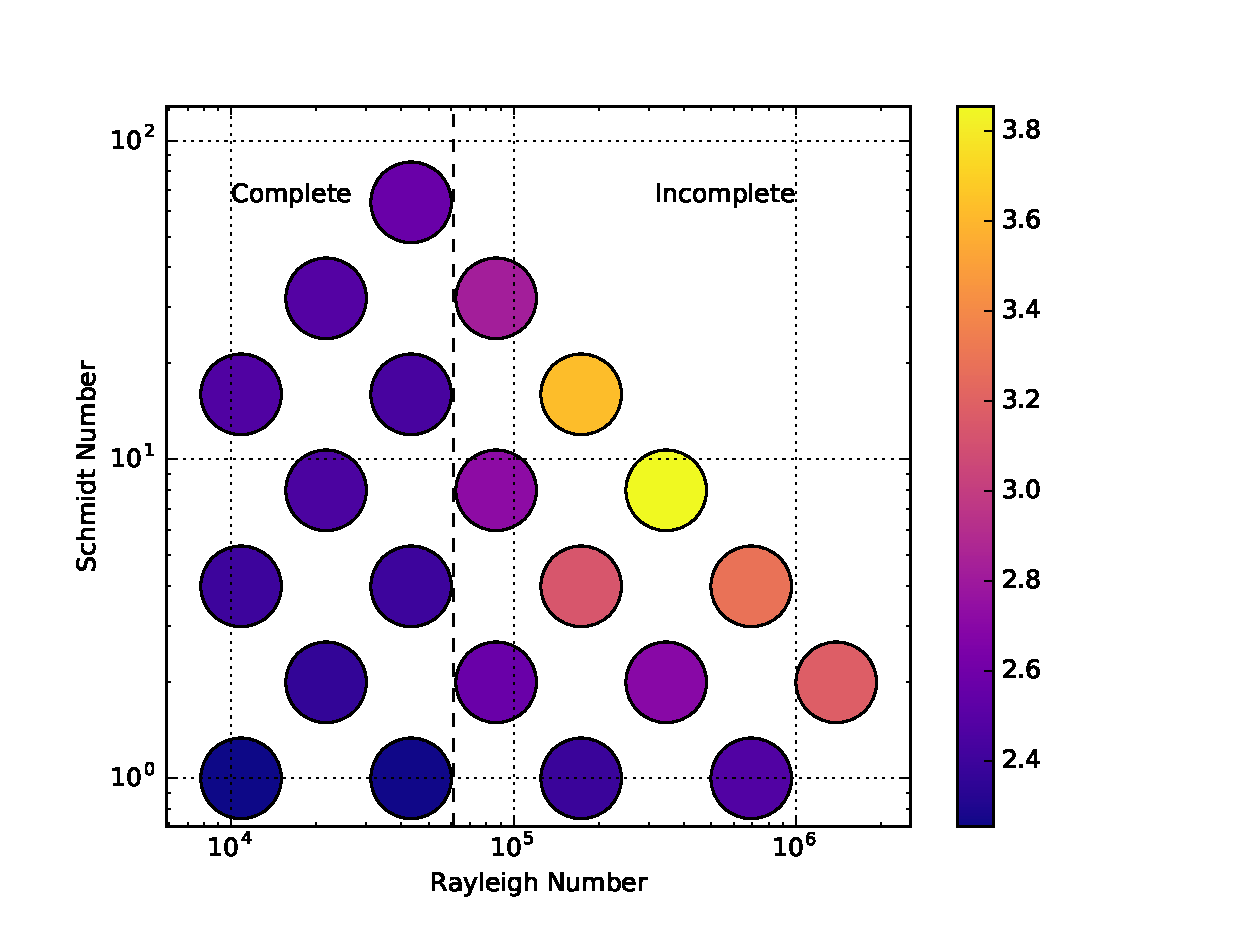
\includegraphics[width=\columnwidth]{figs/C5-vs-Rayleigh-Schmidt}
\caption{ \flabel{C5VsParam}
  Best fit for $C_5$ versus Rayleigh and Schmidt numbers.
  Experiments on the left side of the dashed line completed when the bubble stopped rising.
  Experiments on the right side of the dashed line are incomplete, having approached the vertical boundaries of the simulated domain.
}
\end{figure}

The parameter $C_5$ gives the ratio of the span-wise circumference of the scalar interface to the wavelength.
If the bubble were rectangular in cross section with diameter $\lambda / 2$, then $C_5 = 4$.
If the bubble had a circular cross section with diameter $\lambda / 2$, then $C_5 \approx \pi$.
If the bubble diameter is less than a half-wavelength, then $C_5 < \pi$.
The mixing width $\delta$ increases with time, so the $C_5$ term is most influential at late times.
Therefore, the values of $C_5$ in the incomplete trajectories should be taken with a grain of salt.

The fit values of $C_5$ are plotted versus the Rayleigh and Schmidt numbers in \fref{C5VsParam}.
Among the completed trajectories, $C_5$ is a much stronger function of the Schmidt number than the Rayleigh number, increasing in both.
The values are between 2 and 3, indicate a thinning of the bubble that decreases the mix rate by reducing surface area and total quantity of pure light fluid transported into the dense fluid.

The incomplete trajectories contain richer behavior, with a local maximum at $\text{Ra} = 10^{5.5}$ and $\text{Sc} = 8$.
In aggreate, higher Rayleigh number trajectories have increasing $C_5$ with decreasing diffusivity.
The dependence on the Grashof number is peaked at $\text{Gr} \approx 4.3 \times 10^4$.
The increasing $C_5$ with increasing Schmidt number in the completed trajectories is consistent with these two effects, which can be seen the smoothness of \fref{C5VsParam}.

A possible mechanism for increasing $C_5$ with decreasing diffusivity is the development of structures on the scalar interface the increase the effective surface area.
This is related to the Kelvin-Helmholtz structures proposed to explain increasing $C_2$ with Grashof number, but with additional dependence on the diffusivity which can otherwise smear out the structures.

Another possible mechanism is a change in the bubble diameter.
Higher Grashof number bubbles have thinner momentum boundaries, allowing more buoyant fluid to flow freely through the stem of the bubble.
This sustains the bubble diameter at late times, while more viscous bubbles can thin.
This would explain an increase of $C_5$ with the Grashof number.

The authors have no mechanism by which to explain the local maximum value, so we expect it to disappear with trajectory completion by default.
It would be very interesting if it remained, and further motivates completing the high Rayleigh number trajectories.

\subsubsection{Pure fluid coefficient, $C_7$}
\begin{figure}
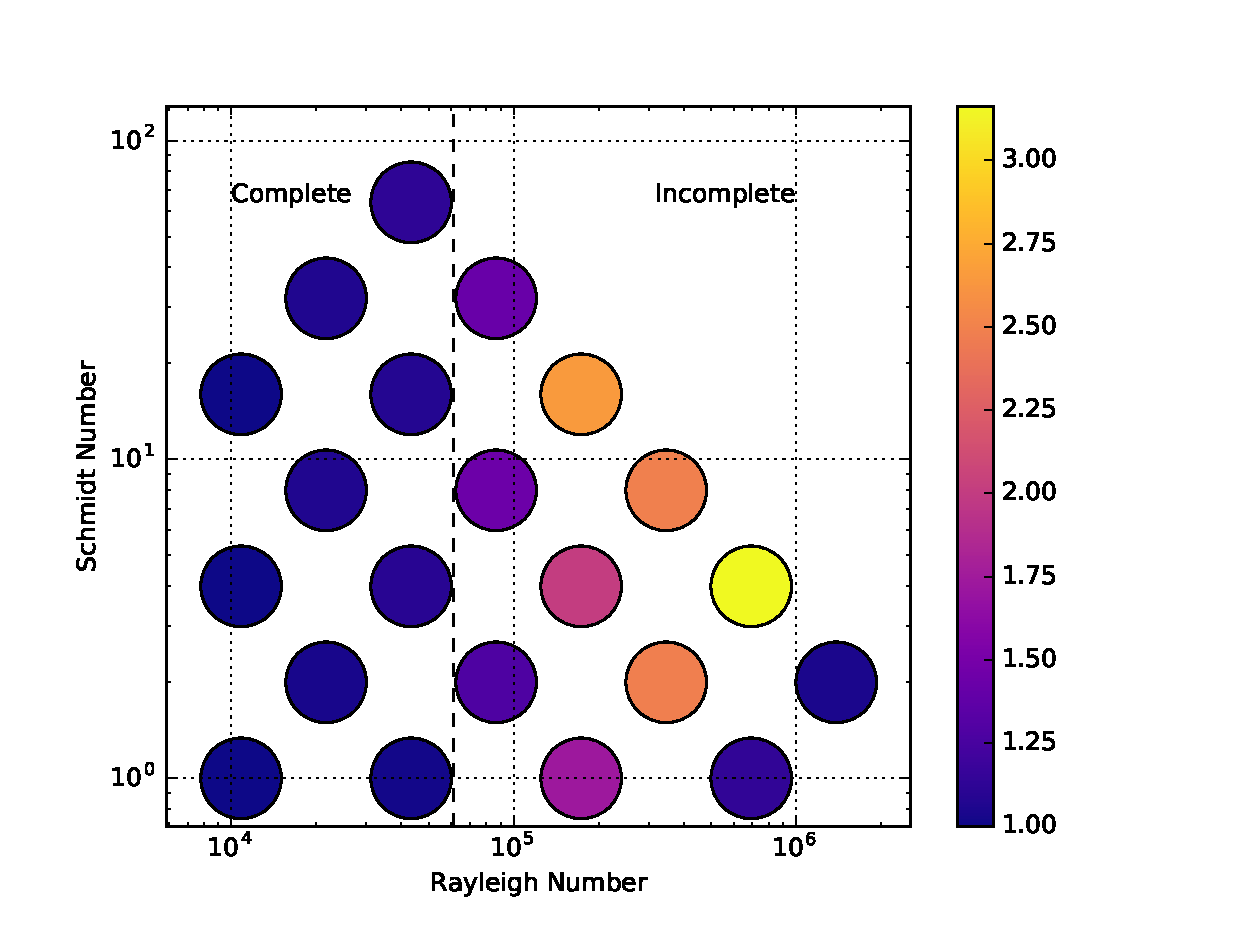
\includegraphics[width=\columnwidth]{figs/C7-vs-Rayleigh-Schmidt}
\caption{ \flabel{C7VsParam}
  Best fit for $C_7$ versus Rayleigh and Schmidt numbers.
  Experiments on the left side of the dashed line completed when the bubble stopped rising.
  Experiments on the right side of the dashed line are incomplete, having approached the vertical boundaries of the simulated domain.
}
\end{figure}

Similar to $C_3$, $C_7$ gives the ratio of the buoyant volume to the maximal mixed volume.
A value of $C_7 = 1$ implies the effective Atwood number is zeroed when $M(t) = \lambda^2 h$.
Values greater than one imply that some portion of the positively buoyant fluid that would be in bubble has become entrained into the neighboring spike, allowing $M(t) > \lambda^2 h$ while retaining net buoyancy.

The fit values of $C_7$ are plotted versus the Rayleigh and Schmidt numbers in \fref{C7VsParam}.
The complete trajectories all have $C_7 \approx 1$, while the incomplete trajectories at higher Rayleigh numbers have increasing $C_7$.
It is possible that at higher Rayleigh numbers some volume of light fluid detaches from the bubble and is transported into the spike.
However, it is more likely that in the incomplete cases $C_7$, which influences the dynamics most at high mixing volumes, is underconstrained.
In that case, we would expect $C_7 \approx 1$ with no dependence on the Grashof, Rayleigh, or Schmidt numbers when the trajectories are completed.




\section{Conclusions} \slabel{conc}

% We proposed a model
We have proposed a simple ODE model for the growth of single mode Rayleigh-Taylor bubbles and spikes at low Atwood number.
The model targets an intermediate range of Grashof numbers and high Rayleigh numbers, in which the single mode perturbation grows into an array of coherent bubbles and spikes.
The dynamics of the bubbles are described in terms of buoyancy, viscous drag, and form drag.
The buoyant force is scaled by a mixing factor related to the volume faction of mixed fluid within the bubble, which is modeled by diffusion across the bubble's interface.

% The coefficients can be connected to the regimes of the flow
We have presented high fidelity spectral element simulations that reach later times and higher aspect ratios than previously available.
The trajectory of the bubble can be roughly divided into regimes based on which terms in the model must be included
The first regime is exponential growth, which requires only the $C_4$, $C_6$, and $C_8$ terms, each of which is set by the linear theory.
Next is the saturation regime, which adds the $C_3$ inertial term and onsets around $h = 0.05 \lambda$.
The $C_1$ form drag term can be added for better agreement, but doesn't change the dynamics qualitatively.
Next is the viscous regime, which adds the $C_2$ skin drag term and onsets around $10^{-4} \text{Gr}$.
The last is the diffusive regime, which adds the $C_5$ and $C_7$ mixing terms and onsets around $10^{-4} \text{Ra}$.

% Stagnation/reacceleration is a transient
The model proposed here is unable to describe stagnation and re-acceleration seen at higher Grashof numbers.
However, the model is very accurate both before and after stagnation and re-acceleration, respectively.
This demonstrates stagnation and re-acceleration to be transients in the flow, occurring around $h = \lambda$, suggesting that the physical processes that lead to them are initially absent, grow to some critical extent, and then decay relative to the magnitude of other processes.
The bubble tip vortex ring is a strong candidate, as suggested by others~\cite{Banerjee2011, Ramaprabhu2012}.
The model could be extended to account for the build-up of vorticity at the bubble tip.

% Viscosity sets the only terminal length scale
The viscous drag, which is absent in other buoyancy-drag models, is essential to recovering terminal behavior at high aspect ratios and low diffusivity.  
Without viscous drag or mixing, the buoyant force grows with the aspect ratio while the form drag does not, leading to unbounded bubble velocity.
In practice, as the velocity grows at high Reynolds number, the bubble interface breaks up leading to enhanced turbulent mixing.
At moderate Reynolds number, viscosity bounds the bubble velocity, generally above the bound given by potential flow theories.

% Mixing kills all bubbles
For any non-zero diffusivity, mixing reduces the buoyant force and the bubble ultimately stops rising.
The penetration depth, i.e. the height of the bubble when it stops, scales linearly with the Rayleigh number.
The relation implicitly defines a critical Rayleigh number below which the bubbles do not rise: $\text{Ra}_c \approx 1500$.

% We can constrain 3 model parameters
The proposed model has 8 descriptive parameters, 3 of which are constrained by the linear theory.
These three are the $C_4 \lambda^3$ term in the inertia, the $C_6 \lambda^2$ term in the surface area, and the $C_8 \lambda^3$ term in the bubble volume.
The presence of the $C_4$ term demonstrates that the volume of fluid that begins to circulate at early times is independent of the bubble height.
$C_4$ is an increasing function of the viscosity, indicating that the viscous entrainment increases this volume, resulting in the reduction in growth rate predicted by the linear theory.

% We can estimate the reamining 5
The physical interpretation of the five remaining parameters provides a prior for their value.
Those parameters are similar to a drag coefficient, a friction factor, and three geometric ratios.
The $C_1$ term is estimated by relation to the drag coefficient of a flat plate.
The $C_2$ term is estimated by relation to the Darcy friction factor in a square duct.
The $C_3$ term is estimated as unity such that the inviscid immiscible acceleration is $Ag$.
The $C_7$ term is estimated as unity such that the fully mixed Atwood number is zero.
The $C_5$ term is estimated as $\pi$, which corresponds to cylindrical bubbles with diameter $\lambda / 2$.

% The parameters are fit to DNS
To calculate the 5 unconstrained model parameters, we fit the model to a battery of direct numerical simulations at moderate Grashof number, high Rayleigh number, and high aspect ratio.
The simulations provide trajectories for the bubble height and volume of mixed fluid.
The single mixing parameter is fit directly to mixed fluid measurements from numerical simulations.
The remaining four parameters are fit with L2 regularization around the prior estimates.
The resulting model reproduces simulated trajectories with relative errors in the bubble height less than 2\% and in the volume of mixed fluid less than 4\%.

% Certain parameters depend on the Grashof number
The $C_3$ and $C_7$ coefficients, which scale the height in the denominator of \eref{dynamics} and \eref{effective-atwood}, respectively, take values very near unity except for the lowest Rayleigh numbers, in the case of $C_3$ and the incomplete trajectories, in the case of $C_7$.
The $C_1$ drag-type coefficient is typically between $0.3$ and $0.6$, with outliers at zero and above $0.9$.
The authors have no direct explanation for the outliers and suggest they are indirectly caused by other early-time breakdowns in the model.
It is conceivable that adding a vortical term, which would be most pronounced at early times, would align these cases with nominal range of values.
The $C_2$ friction factor-type coefficient is an strongly increasing function of the Grashof number and weakly increasing function of the Schmidt number, suggesting that shear instabilities could be enhancing the transport of momentum and consequently the drag.
Similarly, the $C_5$ mixing area coefficient is decreasing with diffusivity, suggesting the development of structure on the interface is smoothed in the diffusive cases.
The $C_5$ coefficient has a peaked dependence on the Grashof number, with a local maximum internal to the simulated trajectories.
The authors have no explanation.

% This is just a start
While the simple model is sufficient to describe coherent, steady bubbles and spikes at low Atwood numbers and high Peclet numbers, few real flows fall within this regime.
In this regard, the simple model proposed here is just one example of a general approach to defining models as a general force balance with coefficients based on limiting cases and simulation data.

The data presented here is a relatively sparse sample of Rayleigh-Schmidt space, intended to explore the efficacy and sensitivity of the model and its coefficients on the governing parameters of the problem.
The model is predictive, in that it can predict the trajectory of the bubble from the initial condition.
However, the model is sensitive to variations in the model coefficients, particularly $C_2$, and $C_5$, that themselves depend on the Rayleigh and Schmidt numbers..
To predict a bubble trajectory for a case within the convex hull of the parameter space explored here, but not at one of those points, the coefficients would need to be interpolated.
For accurate interpolation, the parameter space should be more thoroughly sampled and the interpolation cross-validated.

\section{Acknowledgements}
M. H. acknowledges helpful conversations with Robert Rosner, Aleksandr Obabko, and especially Elizabeth Hicks, and the support of a Department of Energy Computational Science graduate fellowship.

For computer time, this research partially used the resources of the
Supercomputing Laboratory at King Abdullah University of Science \& Technology
 (KAUST) in Thuwal, Saudi Arabia.
This research used resources of the Argonne Leadership Computing Facility, which
is a DOE Office of Science User Facility supported under Contract DE-AC02-06CH11357.








\chapter{Direct numerical simulation of single mode three-dimensional Rayleigh-Taylor experiments}

\section{Abstract}
The single-mode Rayleigh-Taylor instability (smRTI) is well defined, poorly understood, and applicable to many fluid flows directly and through its relationship to multi-mode Rayleigh-Taylor models.
This study reproduces three low-Atwood smRTI experimental runs (Wilkinson and Jacobs, 2007) in
a specialized version of the Nek5000 spectral element code.
The simulations use the initial amplitude, wavelength, acceleration, Atwood number, and viscosity from 
the three specific experiments and impose no-slip and no-flux boundaries on the velocity and scalar, respectively.
The simulations are shown to reproduce the linear, saturation, stagnation, and re-acceleration phases of the smRTI
seen in the experiments.
Additionally, access to the full velocity and scalar fields demonstrates three different finite size effects: 
wall drag, wall lift, and a long wavelength mode along the diagonal.
One of the simulations is extended by a factor of two in the vertical direction and the resulting late-time dynamics
reach Froude numbers around 1.8, higher than previously reported.
Finally, inspection of the span-wise flow reveals secondary flows of the first kind that transport the scalar 
from the bubble-spike interfaces into the bubble and spike centers.
The agreement between simulations and experiments inspires confidence in the spectral element method for studying
the Rayleigh-Taylor instability.


\section{Introduction}

The Rayleigh-Taylor instability occurs when a denser fluid is supported by a lighter one.
Low-amplitude perturbations in the interface between the two fluids grow exponentially with a rate that is well modeled by linear stability analysis~\cite{Duff1962}:
\begin{equation} \elabel{duff}
\gamma = \sqrt{\frac{Agk}{\psi} + \nu^2 k^4} - (\nu + D) k^2,
\end{equation}
where 
$g$ is the local acceleration,
$k$ is the wave-number,
$\nu$ is the kinematic viscosity,
$D$ is the diffusivity,
$A$ is the Atwood number, which characterizes the density difference:
\begin{equation}
	A = \frac{\rho_h - \rho_l}{\rho_h + \rho_l},
\end{equation}
and $\psi$ describes the effect of the interface thickness and is a function of $A$, $k$, and the thickness $\delta$.
In the low Atwood number limit:
\begin{equation}
	\psi = 1 + \frac{k \delta}{\sqrt{\pi}} .
\end{equation}

At larger amplitudes, the perturbations grow non-linearly with the light fluid rising through the heavier fluid in `bubbles' and the heavy fluid falling through the lighter fluid in `spikes.'
Early experiments by Davies and Taylor~\cite{Davies1950a} and potential flow models by Layzer~\cite{Layzer1955} for $A \approx 1$ suggested that the bubbles reach a terminal velocity, and later experiments by Dimonte and Schneider~\cite{Dimonte1996}, also at $A \approx 1$, showed that dense spikes free-fall.
On the other hand, recent experiments by Wilkinson and Jacobs~\cite{Wilkinson2007} and simulations by Ramaprabhu et al.~\cite{Ramaprabhu2006,Ramaprabhu2012}, Wei and Livescu~\cite{Wei2012}, and others~\cite{Sohn2011} show that, at Atwood numbers less than one half, the constant velocity regime is followed by a re-acceleration regime in which the velocity doubles.
The dynamics beyond re-acceleration have not been established, with Ramaprabhu et al. observing a return to the velocity of potential flow~\cite{Goncharov2002} while Wei and Livescu report continued constant acceleration.

Here, we consider the low-Atwood number limit.
The Boussinesq approximation, which ignores density differences that don't multiply the gravitational acceleration, simplifies the governing equations to a single incompressible phase with an active scalar representing the buoyancy:
\begin{align} \elabel{boussinesq}
\frac{D}{D t} u &= - \nabla P + \nu \nabla^2 u - A \vec{g} \phi, \\
\frac{D}{Dt} \phi &= D \nabla^2 \phi, \nonumber
\end{align}
where $u$ is the velocity,
$P$ is the pressure, and 
$\phi$ is the scalar that controls the density gradient.
Without loss of generality, we define $-1 \le \phi \le 1$.
These equations have a symmetry under inversion of the scalar and acceleration, $\phi \rightarrow -\phi, \hat{g} \rightarrow -\hat{g}$, so we know the bubbles and spikes have the same dynamics given the same initial conditions.
The parameter space of the equations are described by two non-dimensional numbers: the Grashof number,
\begin{equation} \elabel{grashof}
\text{Gr} = \frac{A g \lambda^3}{\nu^2},
\end{equation}
where $\lambda$ is a characteristic length, and
the Schmidt number,
\begin{equation} \elabel{schmidt}
\text{Sc} = \frac{\nu}{D}.
\end{equation}

We approximate the governing equations numerically using the spectral element method (SEM)~\cite{Deville2002}.
The SEM converges exponentially with respect to spectral order and has purely dispersive errors, making it a natural method for direct numerical simulations of mixing problems.
Unlike pseudo-spectral methods, it handles no-slip boundaries and can evenly sample the interior of the domain.
We use a specialized version of the Nek5000 community code, NekBox~\cite{Hutchinsonb}, customized specifically to study the low Atwood number Rayleigh-Taylor instability.
NekBox restricts the domain to a tensor product of orthogonal bases and employs fast spectral coarse preconditioners for the pressure Poisson equation.
It is roughly an order of magnitude faster than the more general Nek5000.

It is the goal of this study to validate direct numerical simulations of the low-Atwood single mode Rayleigh-Taylor instability in NekBox against the best available experimental data, that from Wilkinson and Jacobs~\cite{Wilkinson2007}.
In the future, we will apply the same numerical methods to the broader question of the late-time dynamics of the low Atwood smRTI.



In \sref{methods}, we review the spectral element method and describe the numerical parameters of the simulations.
In \sref{results}, we compare the numerical and experimental results, extend the domain in extent and time to reach higher aspect ratios, and introduce new behavior in the span-wise flow.
In \sref{concs}, we discuss the validity of our methods for simulating Rayleigh-Taylor flows, the limits of wall-bounded single mode experiments, and the implications of secondary flows to mixing.
%\aref{data} provides access to the source, input, and output files for the numerical methods.

\section{Numerical methods} \slabel{methods}

\subsection{Spectral element formulation}
The governing equations, \eref{boussinesq}, are discretized using the spectral element method~\cite{Deville2002}.
The domain is first divided into cubic elements.
Each element is represented by a tensor product of $n^3$ Gauss-Lobatto-Legendre (GLL) quadrature points of order $p = n-1$.
The elements are coupled by continuity at the shared points on their faces.

Time is discretized with a 3rd order backwards difference formula (BDF3).
The linear and non-linear terms are split, and the non-linear convection operator is extrapolated with a 3rd order scheme that sets the 3rd derivative at the extrapolated point to zero (EX3).
The full discrete system is 3rd order in time, $p$th order in space, and has purely dispersive errors.

Initially, no filtering is applied.
Filtering is applied when the scalar field $\phi$ exhibits small scale oscillations on what should otherwise be smooth steep boundaries.
For Schmidt numbers greater than or equal to unity, the scalar field is less numerically stable than the velocity, so instability in the scalar precedes instability in the velocity.
The filter attenuates the highest frequency mode of the velocity and scalar fields within each element by 5\% at each time-step.

\subsection{Simulation setup}

\begin{figure}
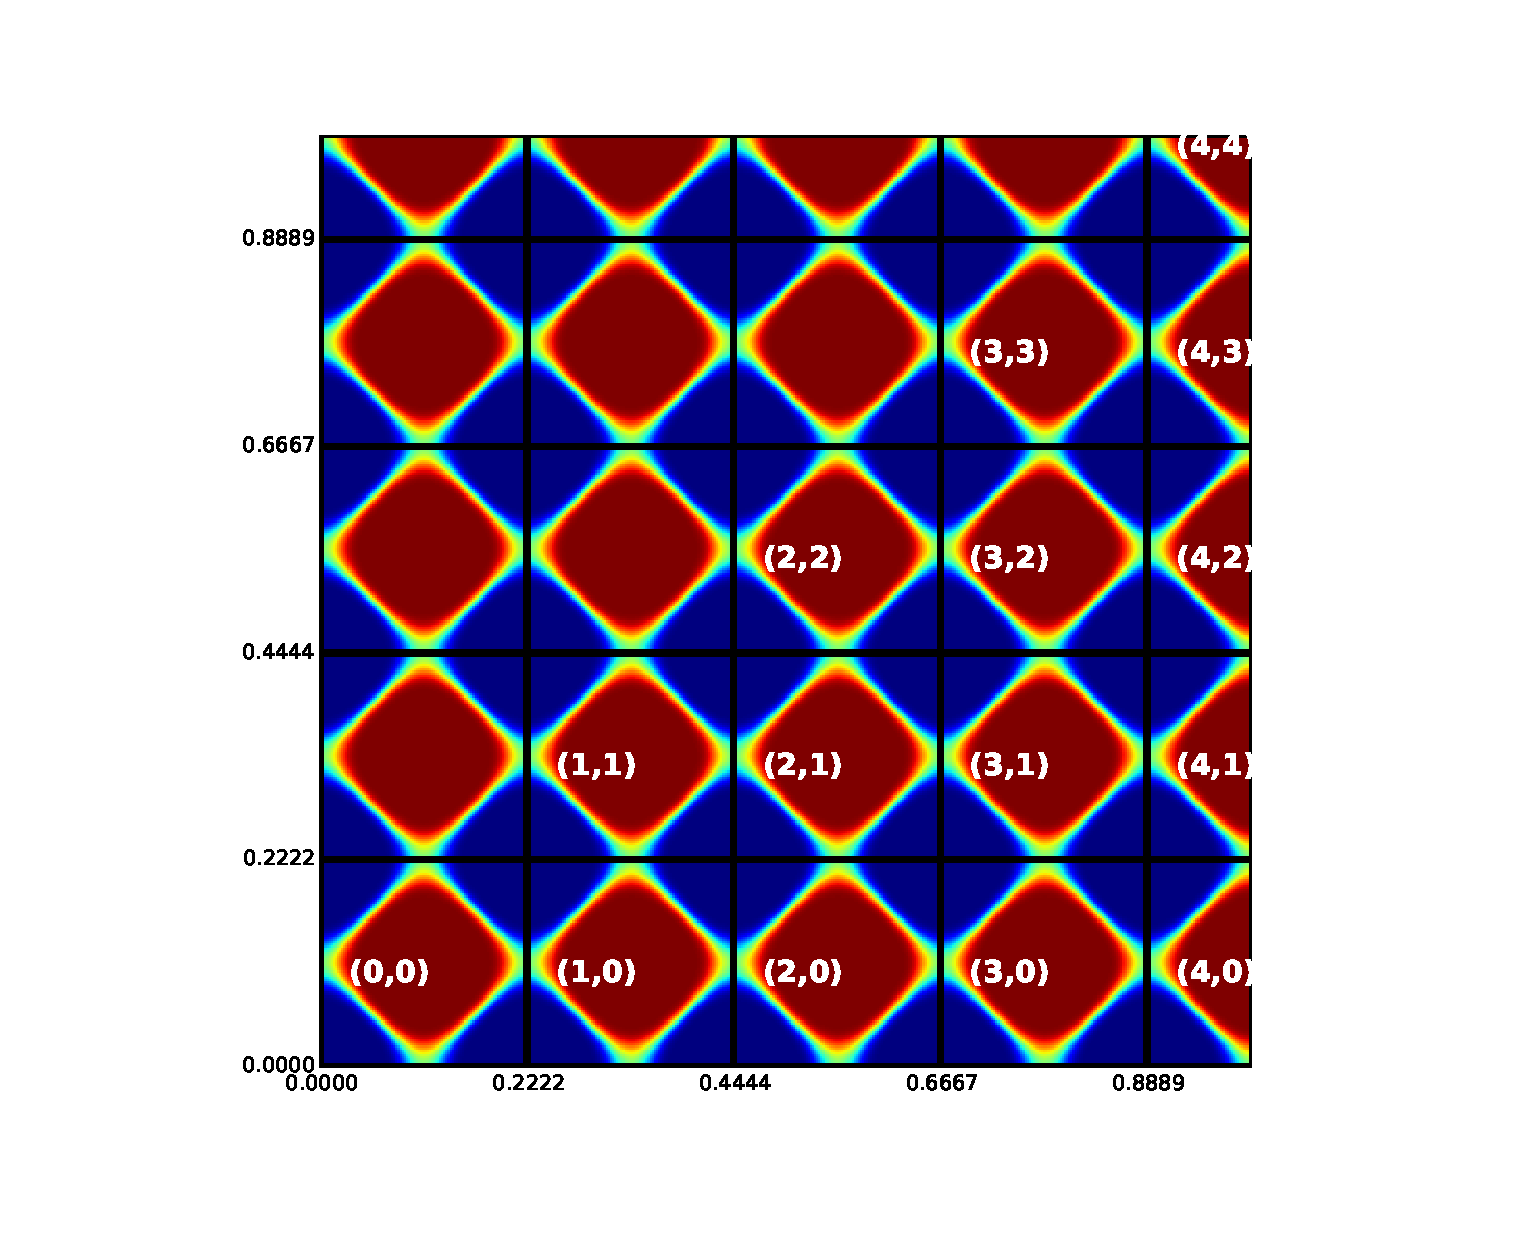
\includegraphics[width=\columnwidth]{figs/cells}
\caption{ \flabel{ic} 
Initial condition, $\phi(x,y,0,0)$, for 4.5 mode simulation.  
The bubbles are logically separated by the solid grid and each unique bubble is labeled.
}
\end{figure}

\begin{table}
\begin{center}
\input{tbl/params.tbl}
\end{center}
\caption{ \tlabel{params}
Parameters of simulations.
The aspect ratio is defined with respect to the quiescent amplitude, $a_0$, from \eref{rollback}.
The last row is the simulation that extends the tank by a factor of two in the vertical direction.
}
\end{table}

Three simulations were conducted to reproduce experiments with 2.5, 3.5, and 4.5 modes across the diagonal.
Then, an extension of the 4.5 mode experiment with twice the vertical extent was performed.
Finally, a 4.5 mode calculation with periodic boundary conditions and unit Schmidt number was performed as a reference for comparing the growth of the bubbles in the wall-bounded flows.

The boundary conditions for the non-periodic simulations are no-slip for the velocity and no-flux (insulating) for the scalar.
The initial conditions for the velocity are quiescent.
The initial conditions for the scalar are the product of two cosines smeared by an error function in the z-direction:
\begin{equation}
  \phi(x,y,z,0) = \text{erf}\left[ \frac{z + a_0 \cos(k_x x) \cos(k_y y)}{\delta} \right] ,
\end{equation}
where $a_0$ is the initial amplitude,
$k_x$ and $k_y$ are the wave-numbers in the x and y directions, respectively, and
$\delta$ is the interface thickness.
In our case, $k_x = k_y$.
An example initial condition is plotted in \fref{ic}.
By symmetry, we know that the average scalar is zero, $H_{i,j} = H_{j,i}$, and that the spike dynamics are identical to the bubbles.

The Atwood number, local acceleration, and initial amplitude where taken from experimental measurements by Wilkinson and Jacobs~\cite{Wilkinson2007, JacobsPrivate}.
In the experiment, the interface has a non-zero initial velocity and the bulk flow is not measured.
Instead of trying to model the bulk flow, we used the linear theory, \eref{duff}, to transform the flow to quiescence.
Specifically, the system
\begin{align} \elabel{rollback}
H &= a_0 \cosh\left(\gamma (t - t_0)\right) \\
V &= a_0 \gamma \cosh\left(\gamma (t-t_0) \right)  \nonumber
\end{align}
where $H$ and $V$ were the experimental measures of the initial interface height and velocity, respectively,
is solved for $a_0$ and $t_0$, the quiescent amplitude and time.
The quiescent amplitude is used for the simulations.
The experiments to reproduce were selected such that solutions to \eref{rollback} existed and the bubble reached the greatest heights.

The viscosity is matched to the experimental fluids, but the diffusivity is not.
The Schmidt number in the experiments is in excess of 1000.
The computational cost of the simulation goes with the Schmidt number to the 4th power, so directly simulating such high Schmidt number was not possible.
Instead, the Schmidt number was varied in the range of 1 to 7 to gain a qualitative understanding of its influence on the flow.

It should be noted that, while the Atwood number was used to scale the local acceleration, the Boussinesq approximation implies that the Atwood number has been taken to zero while keeping the product $Ag$ fixed.
The generally accepted Boussinesq limit is $A = 0.05$, which is three times smaller than the Atwood number in this case.
Previous simulations directed at single-mode re-acceleration have been performed at $A \ge 0.15$, so it is not known whether re-acceleration persists in the limit as $A \rightarrow 0$.

The three simulations reproducing experimental runs are conducted on the Mira supercomputer at Argonne Leadership Computing Facility (ALCF).
The resolution and time-step was chosen to ensure numerical stability: a $256\times256\times512$ mesh of 7th order elements for 11,509,170,176 degrees of freedom.
The simulation was distributed over 524,288 cores and 1,048,576 MPI processes.
64 outputs were written to disk, each 6/8ths of a TiB.
The number of elements and degrees of freedom are doubled for the extension to twice the vertical extent.

\subsection{Post-processing}
The simulation outputs the velocity, pressure, and scalar fields at the Gauss-Lobatto-Legendre points in double precision.
They are post-processed into low-dimensional observables: the bubble height and two-dimensional slices of the velocity, vorticity, pressure, and scalar through the horizontal mid-plane and vertical diagonal.
Post-processing is performed using the `nek-analyze' post-processing framework, which implements a MapReduce-like~\cite{dean2008mapreduce} backend for parallel, out-of-core analysis.

The bubble height is defined as:
\begin{equation} \elabel{h_exp}
H = \sup \left\{ z : \min_{x,y} \phi(x,y,z) < 0\right\},
\end{equation}
which avoids measuring the diffusive growth by tracking the center of the interface profile instead of the ends.
The bubble velocity is found by fitting a cubic spline to $H(t)$ and differentiating.

The height of individual bubbles, $H_{i,j}$, is found by restricting $\min_{x,y}$ in \eref{h_exp} to the span-wise square of diagonal length $\lambda$ centered on the bubble in the $i$-by-$j$-th position.
The bubble domains and labels are shown in \fref{ic}.



\section{Results} \slabel{results}

\subsection{Validation}

\subsubsection{Linear growth rate}

\begin{table}
\input{tbl/linear.tbl}
\caption{ \tlabel{linear}
Growth rate: linear theory vs simulation.
Theoretical values are calculated as in \eref{duff}.
Simulation values are calculated as in \eref{linear_sim}.
The aspect ratio is shown for the second sample, $h_1 / \lambda$.
Note the difference in Schmidt number between the two $4.5$ mode cases.
}
\end{table}

We compute the growth rate from the bubble height at the first simulation output time:
\begin{equation} \elabel{linear_sim}
\gamma \approx \frac{1}{t_1} \text{acosh}\left(\frac{h(t_1)}{h(0)}\right), 
\end{equation}
and collect the results in \tref{linear}.
Because the simulations targeted the non-linear regime, the height is not available until characteristic time $\tau = t \gamma \sim 2$ and aspect ratio $h / \lambda \approx 0.1$.
Therefore, we expect the simulation value to be below the theoretical value given by \eref{duff} due to saturation.

The agreement is good, with only the lower Grashof, higher aspect ratio 4.5 mode calculation deviating more than a part in one hundred.
The 2.5 mode simulation outperforms the theory slightly.
This could be due to the long-wavelength finite size effect discussed later, which is stronger for fewer modes in the finite domain.

\subsubsection{Froude number}

\begin{figure}
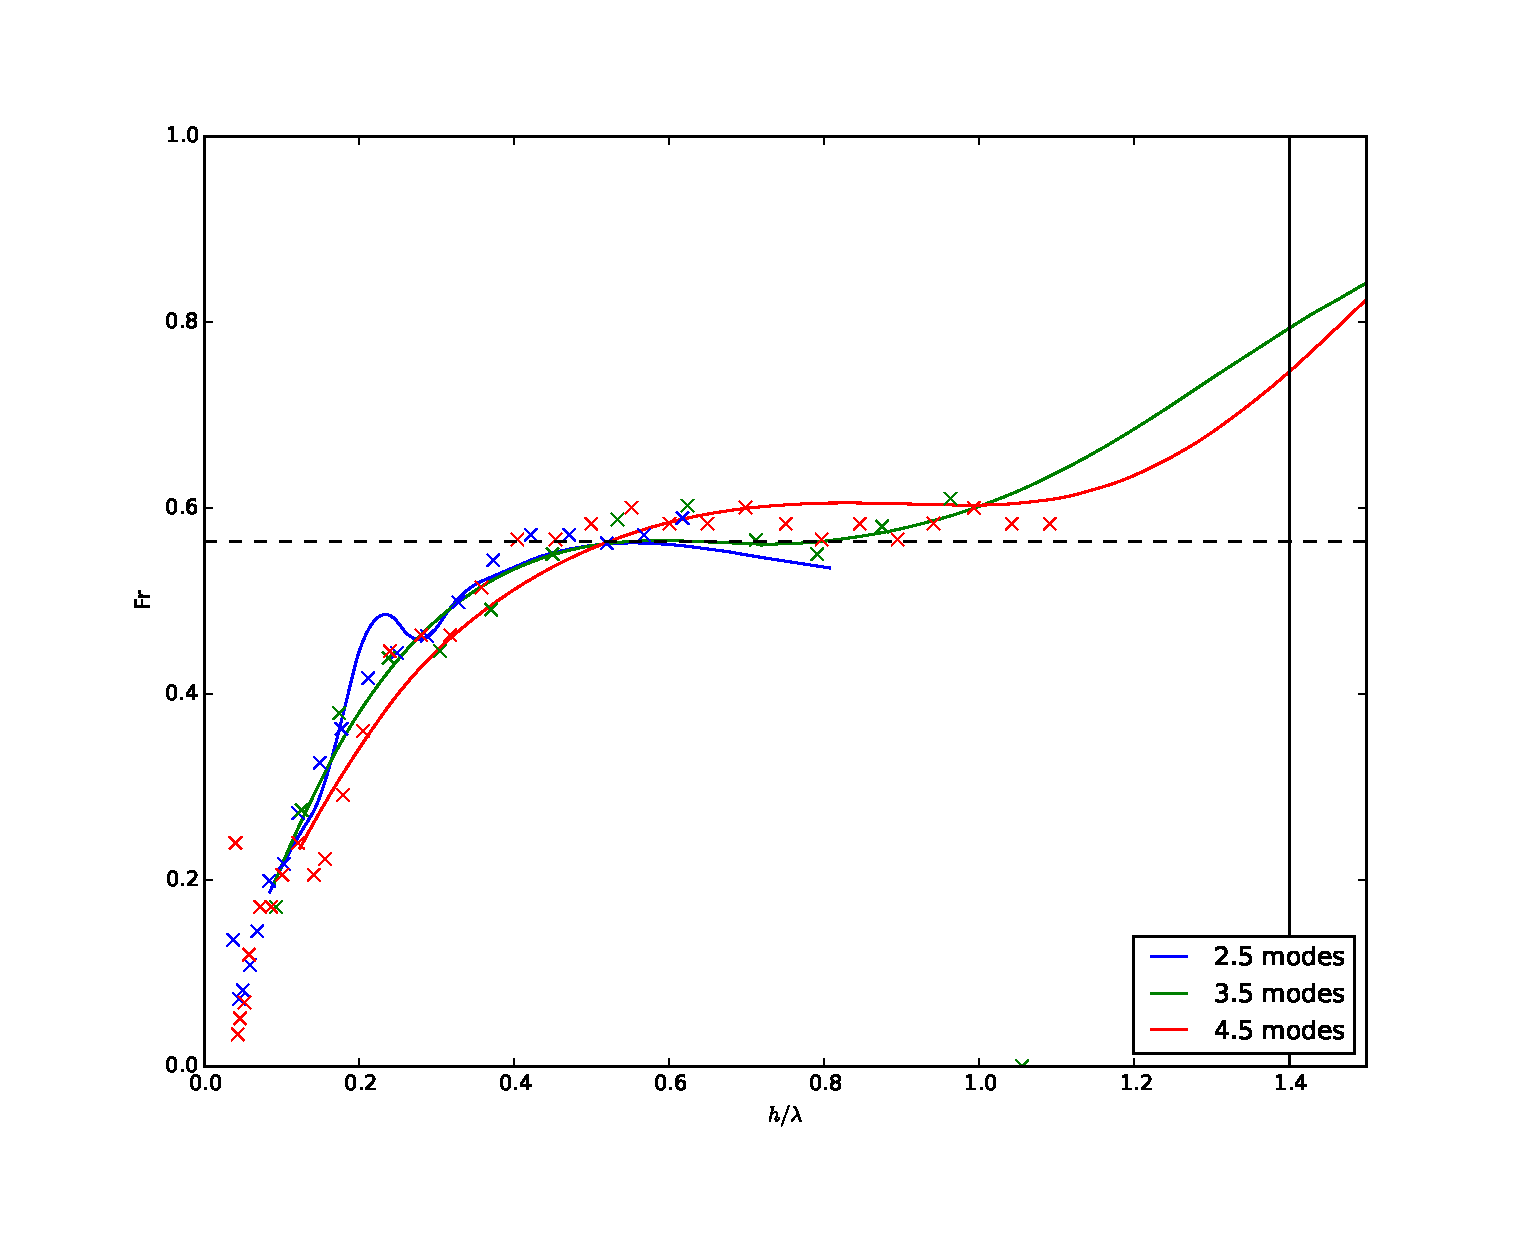
\includegraphics[width=\columnwidth]{plts/Fr}
\caption{ \flabel{froude} 
Froude number vs height, non-dimensionalized by the wavelength.
Lines are the derivative of cubic splines through simulation outputs.
Points are from experiment via direct measurement of the bubble velocity~\cite{JacobsPrivate}.
The dotted horizontal line is positioned at Goncharov's theoretical value of $\pi^{-1/2}$~\cite{Goncharov2002}.
}
\end{figure}

\begin{figure}
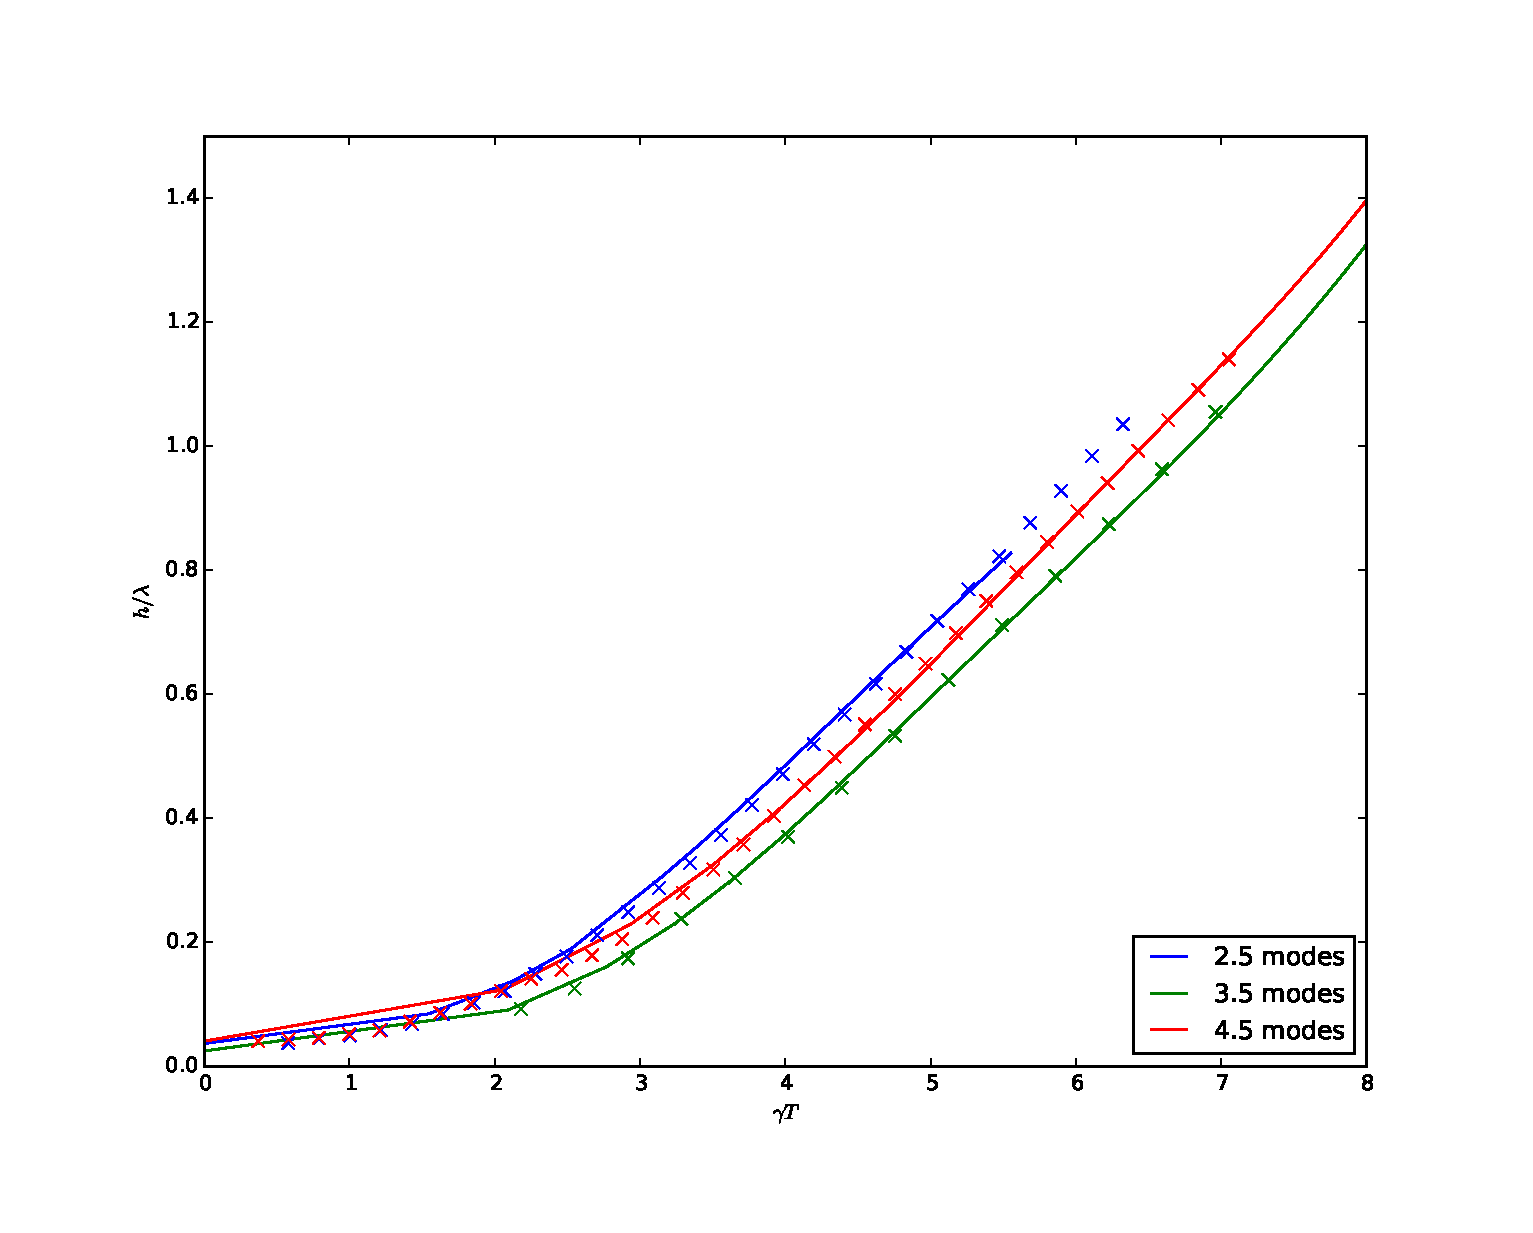
\includegraphics[width=\columnwidth]{plts/aspect}
\caption{ \flabel{aspect} 
Bubble height vs time, non-dimensionalized by the wavelength and linear growth rate, respectively.
Lines are cubic splines through simulation outputs.
Points are from experiment~\cite{JacobsPrivate}.
The points are shifted in time to minimize the square deviation from the spline summed over the plotted points.
}
\end{figure}

The experiments observe only the diagonal plane and measure the height with respect to the most internal bubble.
Therefore, we plot in \fref{froude} the non-dimensional velocity, i.e. the Froude number, of the central bubble alone:
\begin{equation}
	\text{Fr} = \frac{v}{\sqrt{ A g \lambda}}
\end{equation}
In each case, the simulation exhibits the same qualitative behavior as the experiment:
exponential growth saturating to a stagnation velocity around Goncharov's theoretical value of $\text{Fr} = \pi^{-1/2}$~\cite{Goncharov2002}.
In cases where the simulation and experimental data extend in time, the beginnings of re-acceleration are also seen.

The 2.5 mode case exhibits peculiar behavior with two inflection points around aspect ratio $h / \lambda = 0.2$.
This is not an issue with the splines, as can be seen in \fref{aspect}, which plots the non-dimensional height vs non-dimensional time without splines.
The 2.5 mode case, which has the highest Grashof and Schmidt numbers, went unstable.
Upon inspection, the 5\% filtering was unable to suppress the oscillations in the scalar field.
This simulation could be retried with greater resolution, but, given the stability of the 3.5 mode case, the computational cost would be up to 43$\times$ greater, which is why it was not repeated in this study.

\subsection{Extension}

Given the agreement between the simulations and the experiment, we can use the simulations to explore the flow in ways that are not readily accessible experimentally.
In this study, we extend the subject cases and analysis in three ways.
First, we calculate the height of each bubble in the tank individually and use the results to study finite size effects.
Second, we extend the 4.5 mode experiment by a factor of two in the vertical extent of the domain and simulation time to delay interaction with the top boundary and reach later times and larger bubble heights.
Finally, we consider the span-wise, vs stream-wise, flow by taking slices of the midplane and observing pressure driven secondary flows.
These three extensions are a small sample of the types of observations that are available numerically.

\subsubsection{Wall effects}

\begin{figure*}
\begin{subfigure}[b]{\columnwidth}
  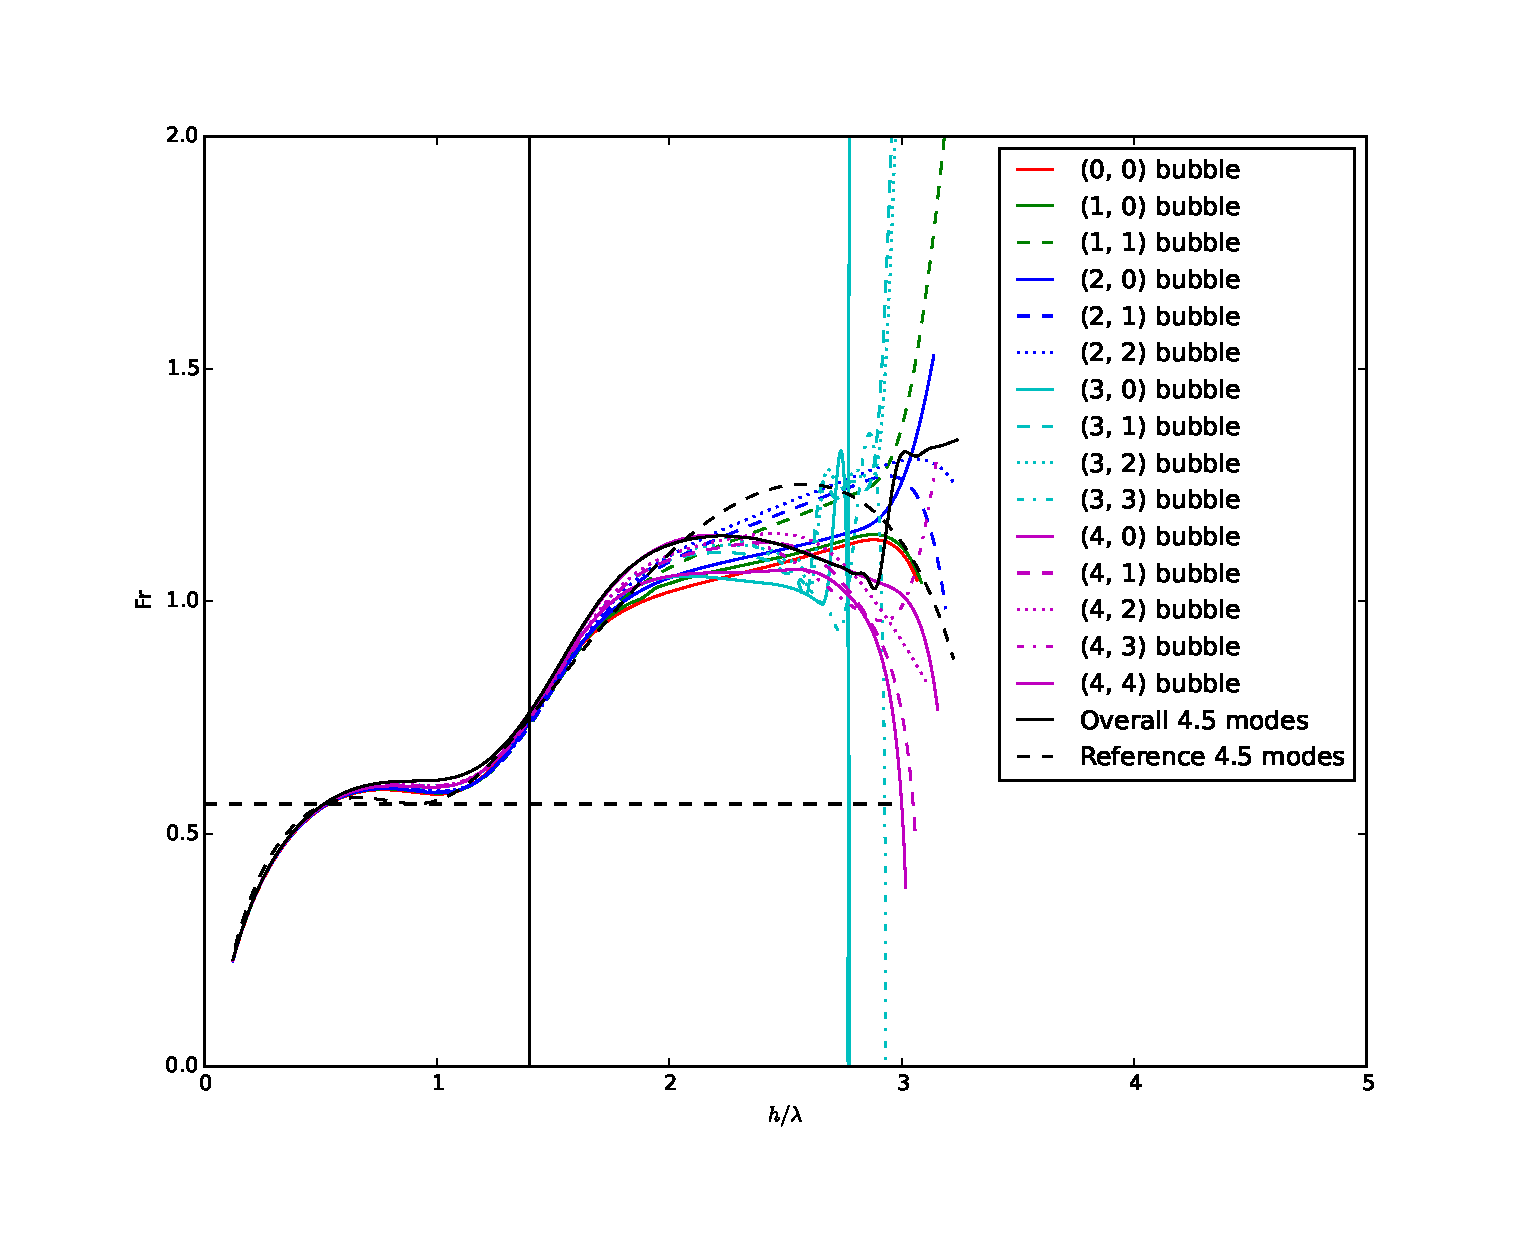
\includegraphics[width=\columnwidth]{plts/walls_Fr}
\end{subfigure}
\begin{subfigure}[b]{\columnwidth}
  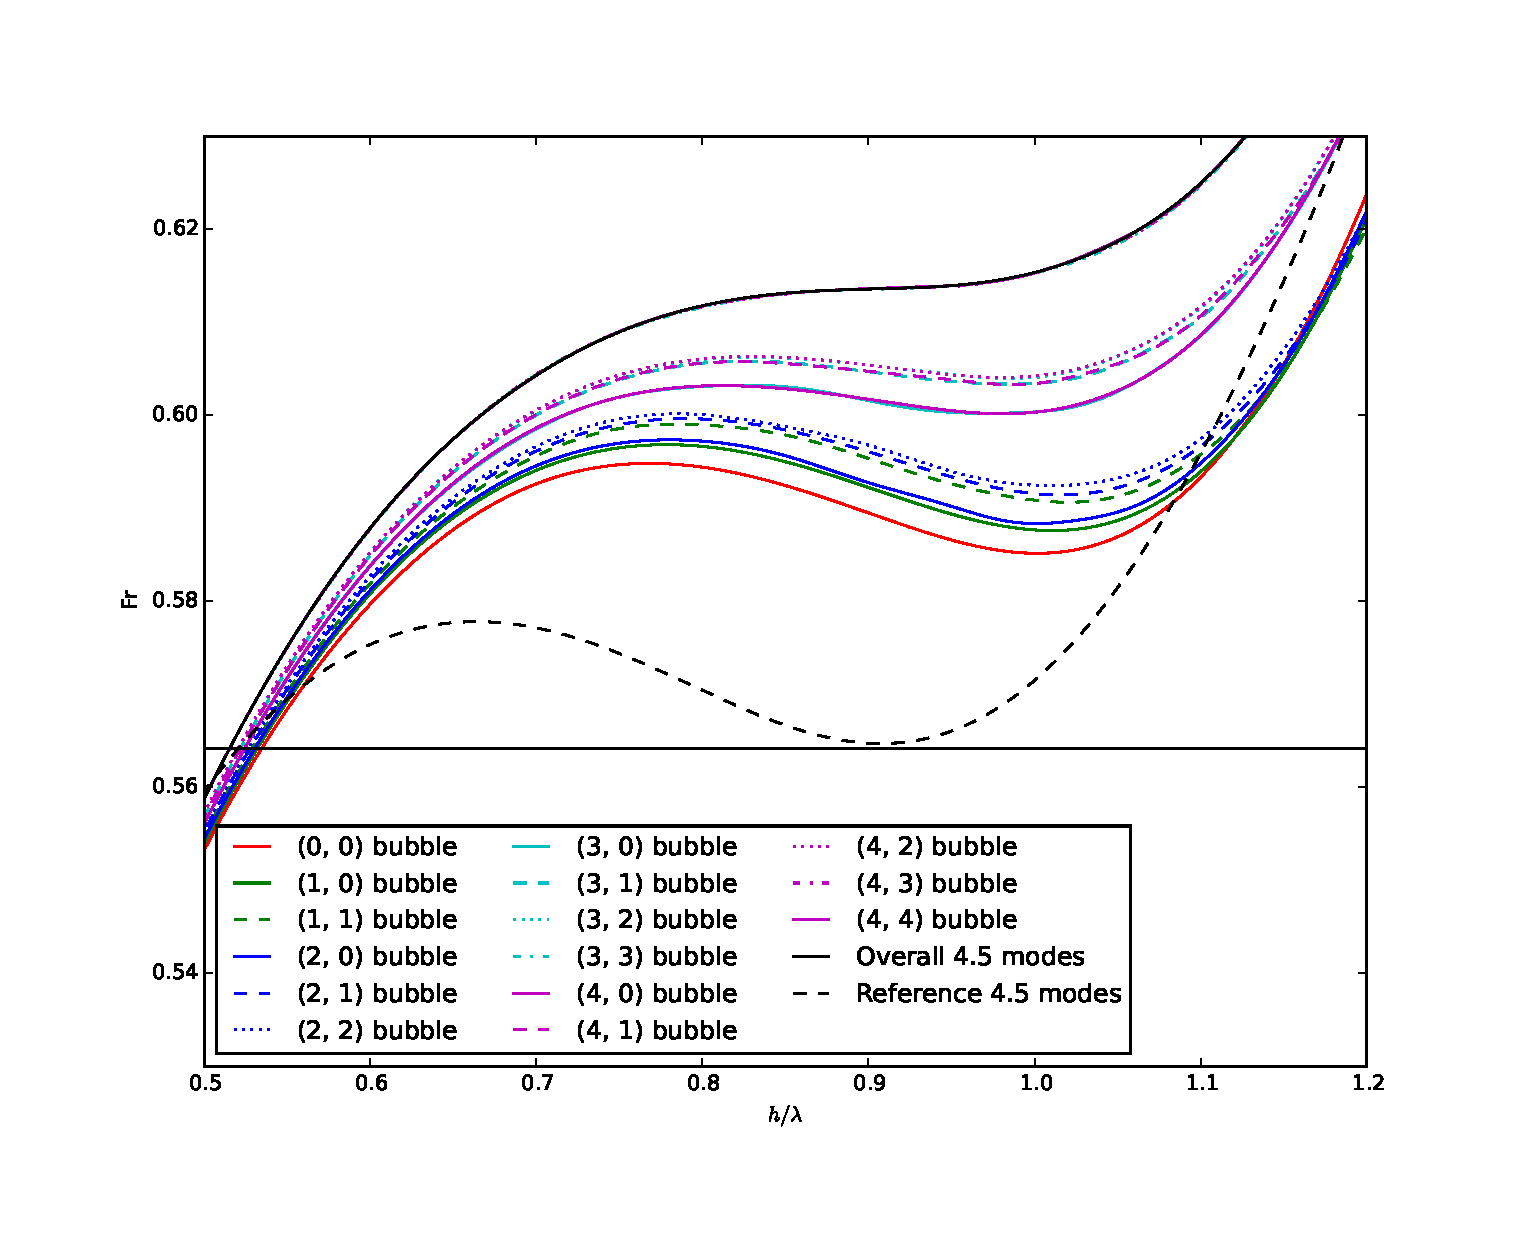
\includegraphics[width=\columnwidth]{plts/walls_Fr_zoom}
\end{subfigure}
\caption{ \flabel{froude_wall} 
Froude number as a function of height, non-dimensionalized by the wavelength, by bubble in the 4.5 mode simulation.
Solid line is from the height defined as the maximum taken over the entire span-wise domain.
Dotted line is the periodic reference calculation.
}
\end{figure*}

\begin{figure*}
\begin{subfigure}[b]{\columnwidth}
  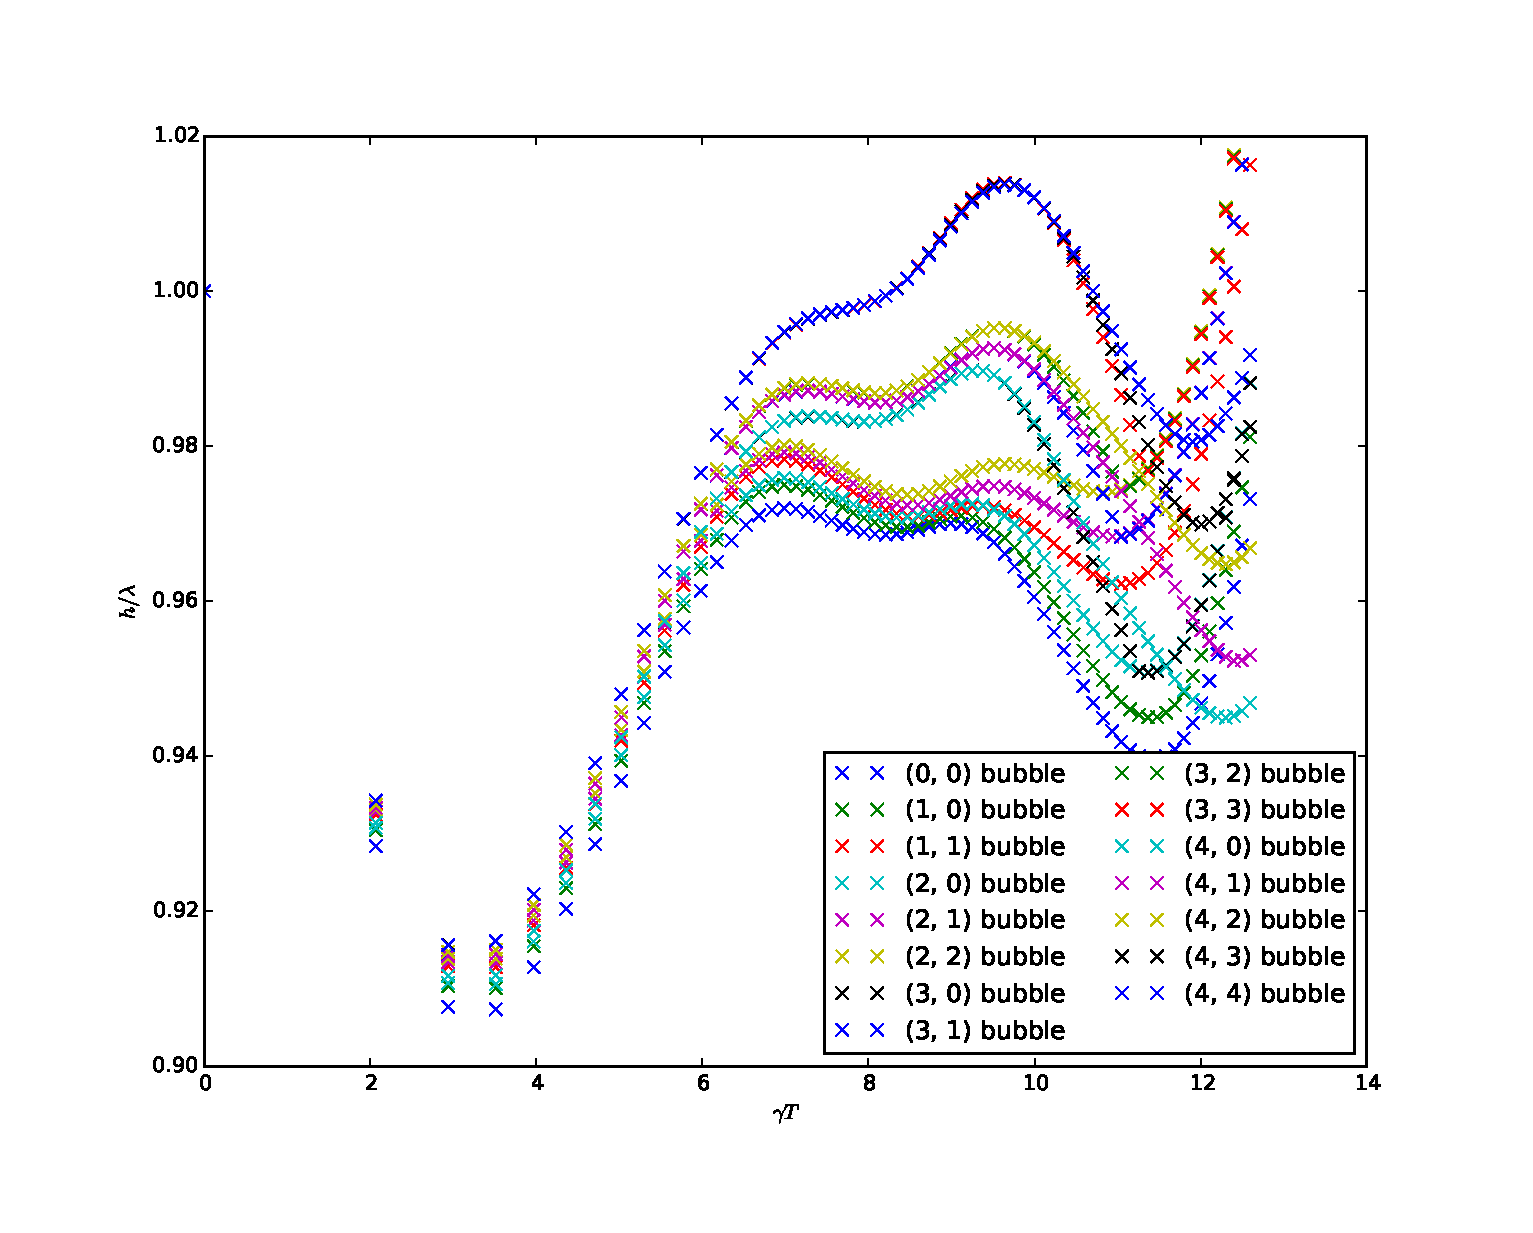
\includegraphics[width=\columnwidth]{plts/walls_h}
\end{subfigure}
\begin{subfigure}[b]{\columnwidth}
  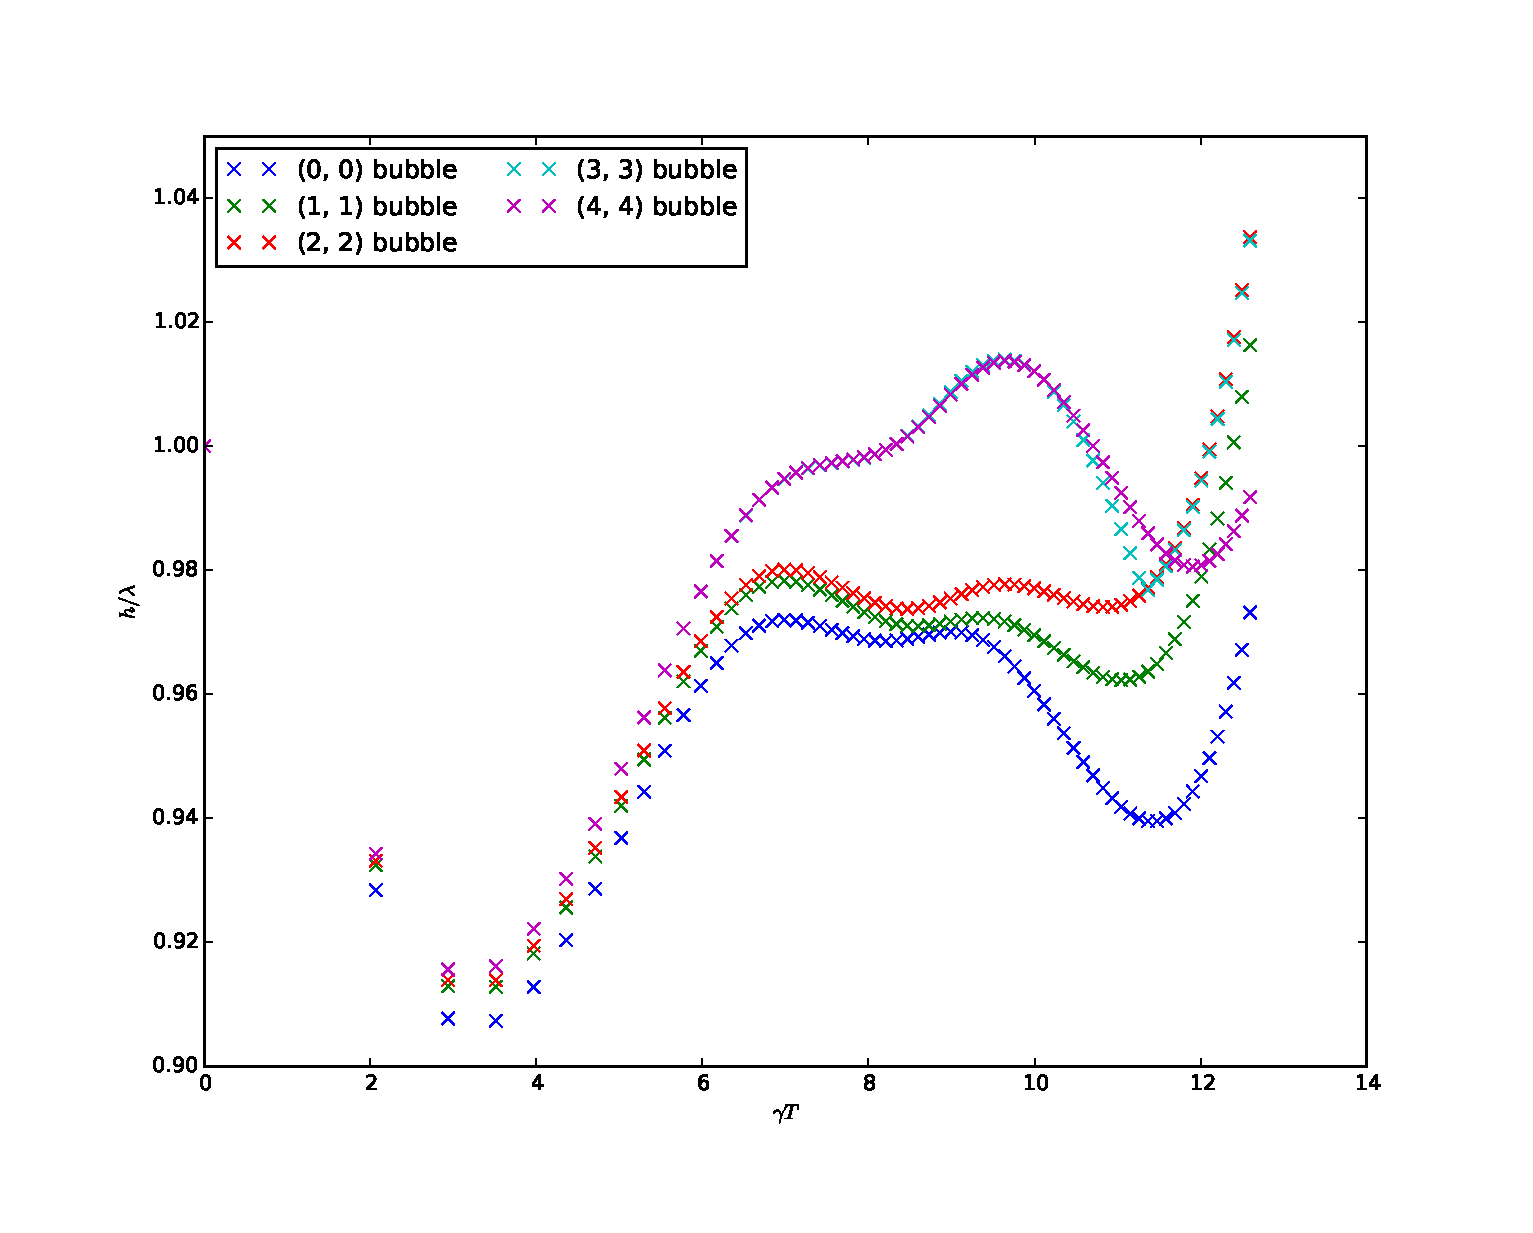
\includegraphics[width=\columnwidth]{plts/walls_h_diag}
\end{subfigure}
\caption{ \flabel{ratio_wall}
Ratio of wall-bounded bubble height to periodic bubble height in the 4.5 mode simulation.
}
\end{figure*}

\begin{figure*}
\begin{subfigure}[b]{0.66\columnwidth}
  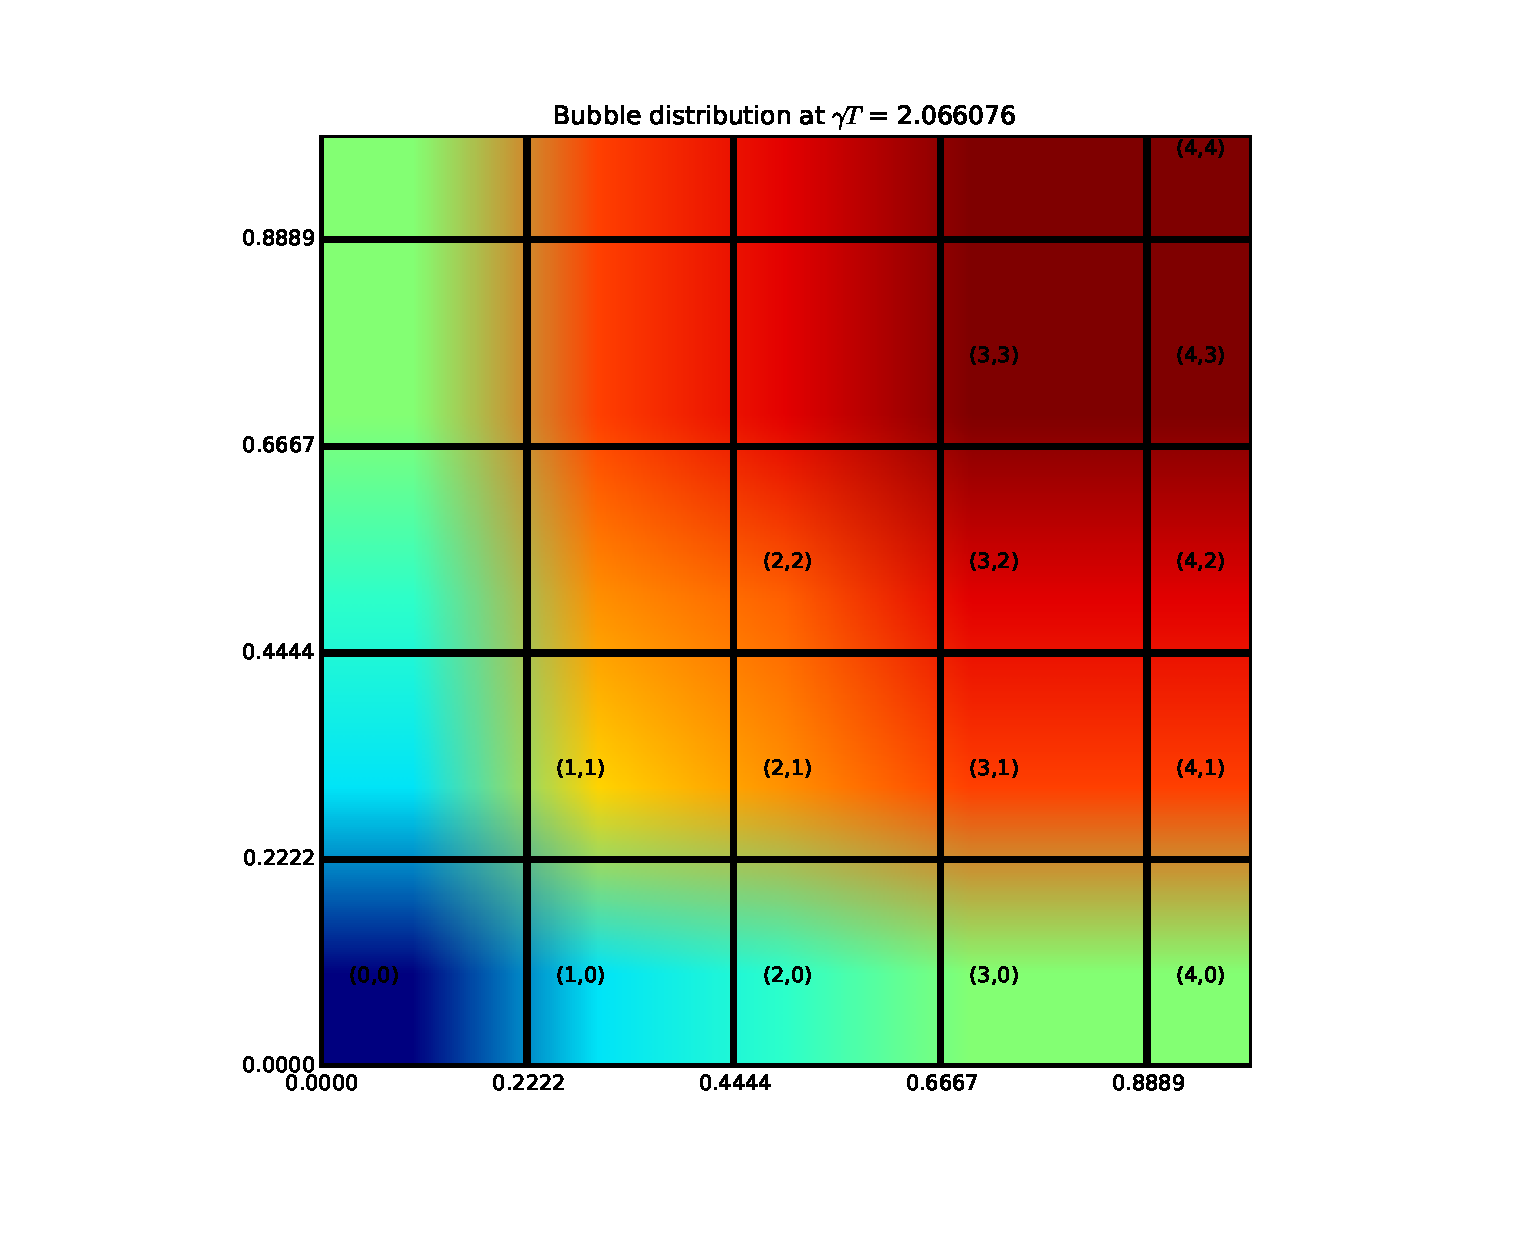
\includegraphics[width=0.66\columnwidth]{figs/spatial_bubble-1}
\end{subfigure}
\begin{subfigure}[b]{0.66\columnwidth}
  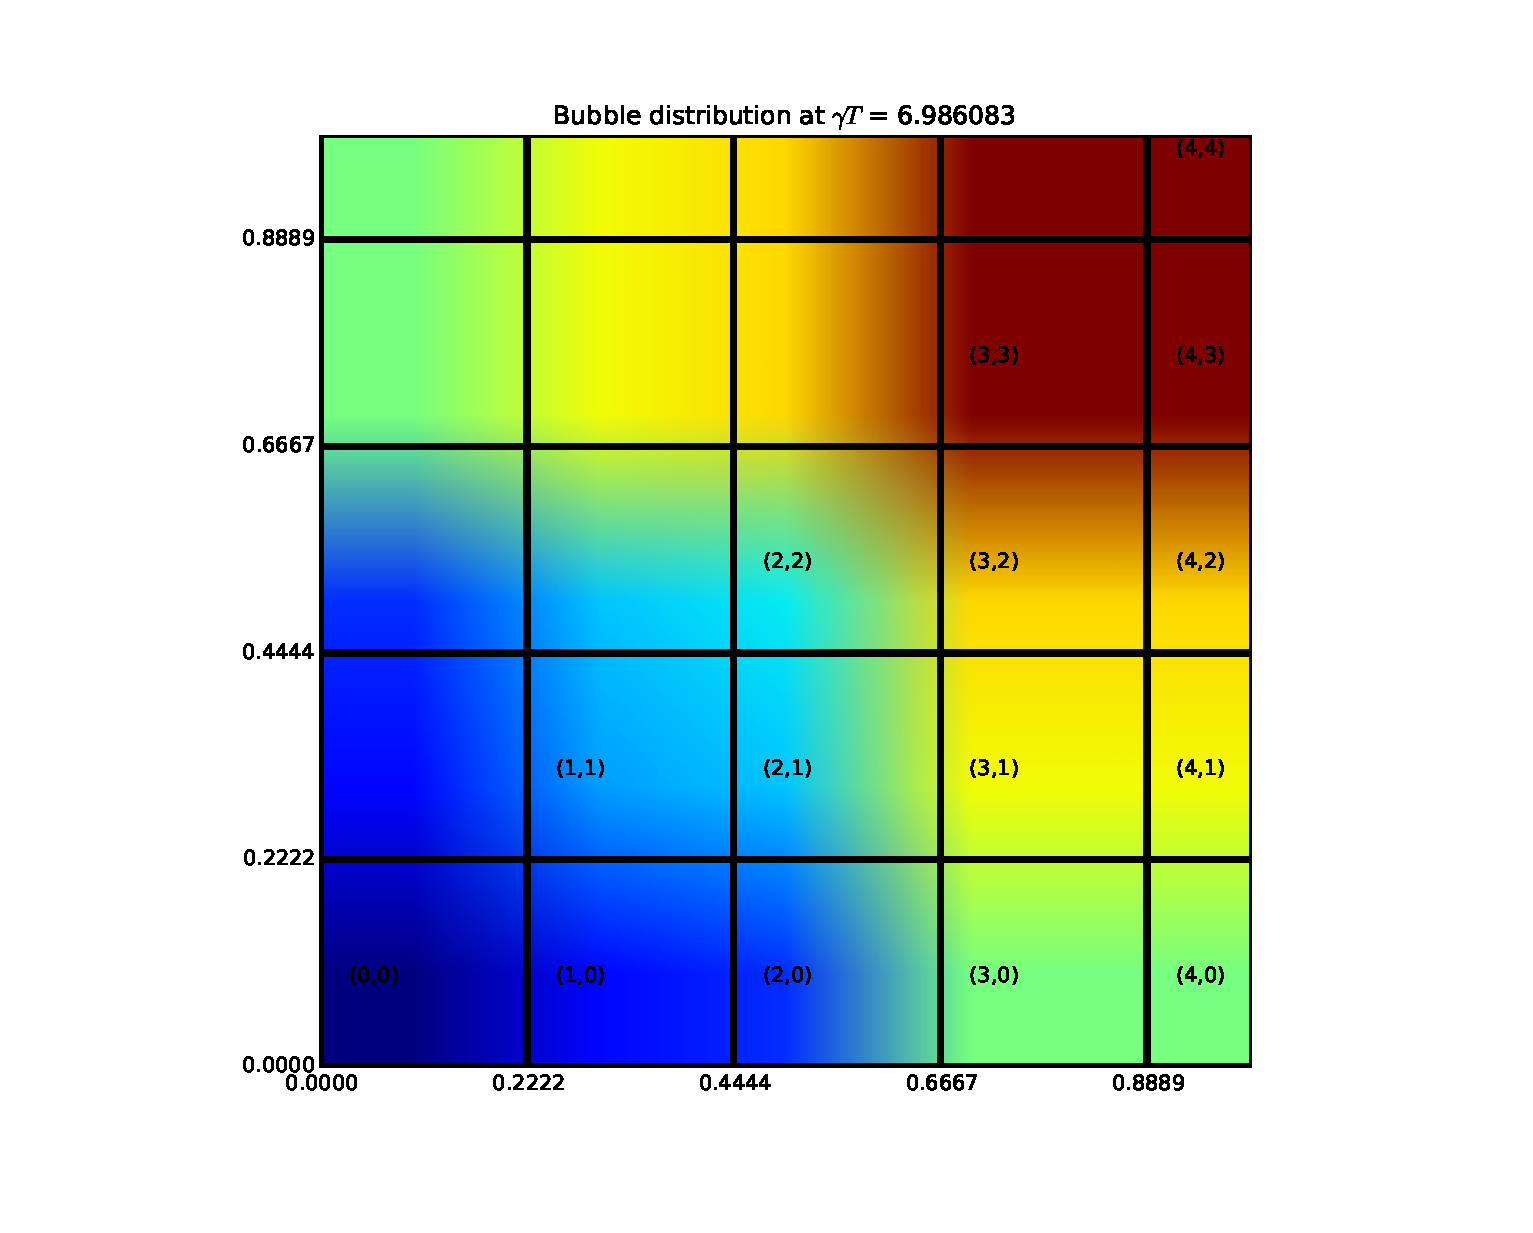
\includegraphics[width=0.66\columnwidth]{figs/spatial_bubble-17}
\end{subfigure}
\begin{subfigure}[b]{0.66\columnwidth}
  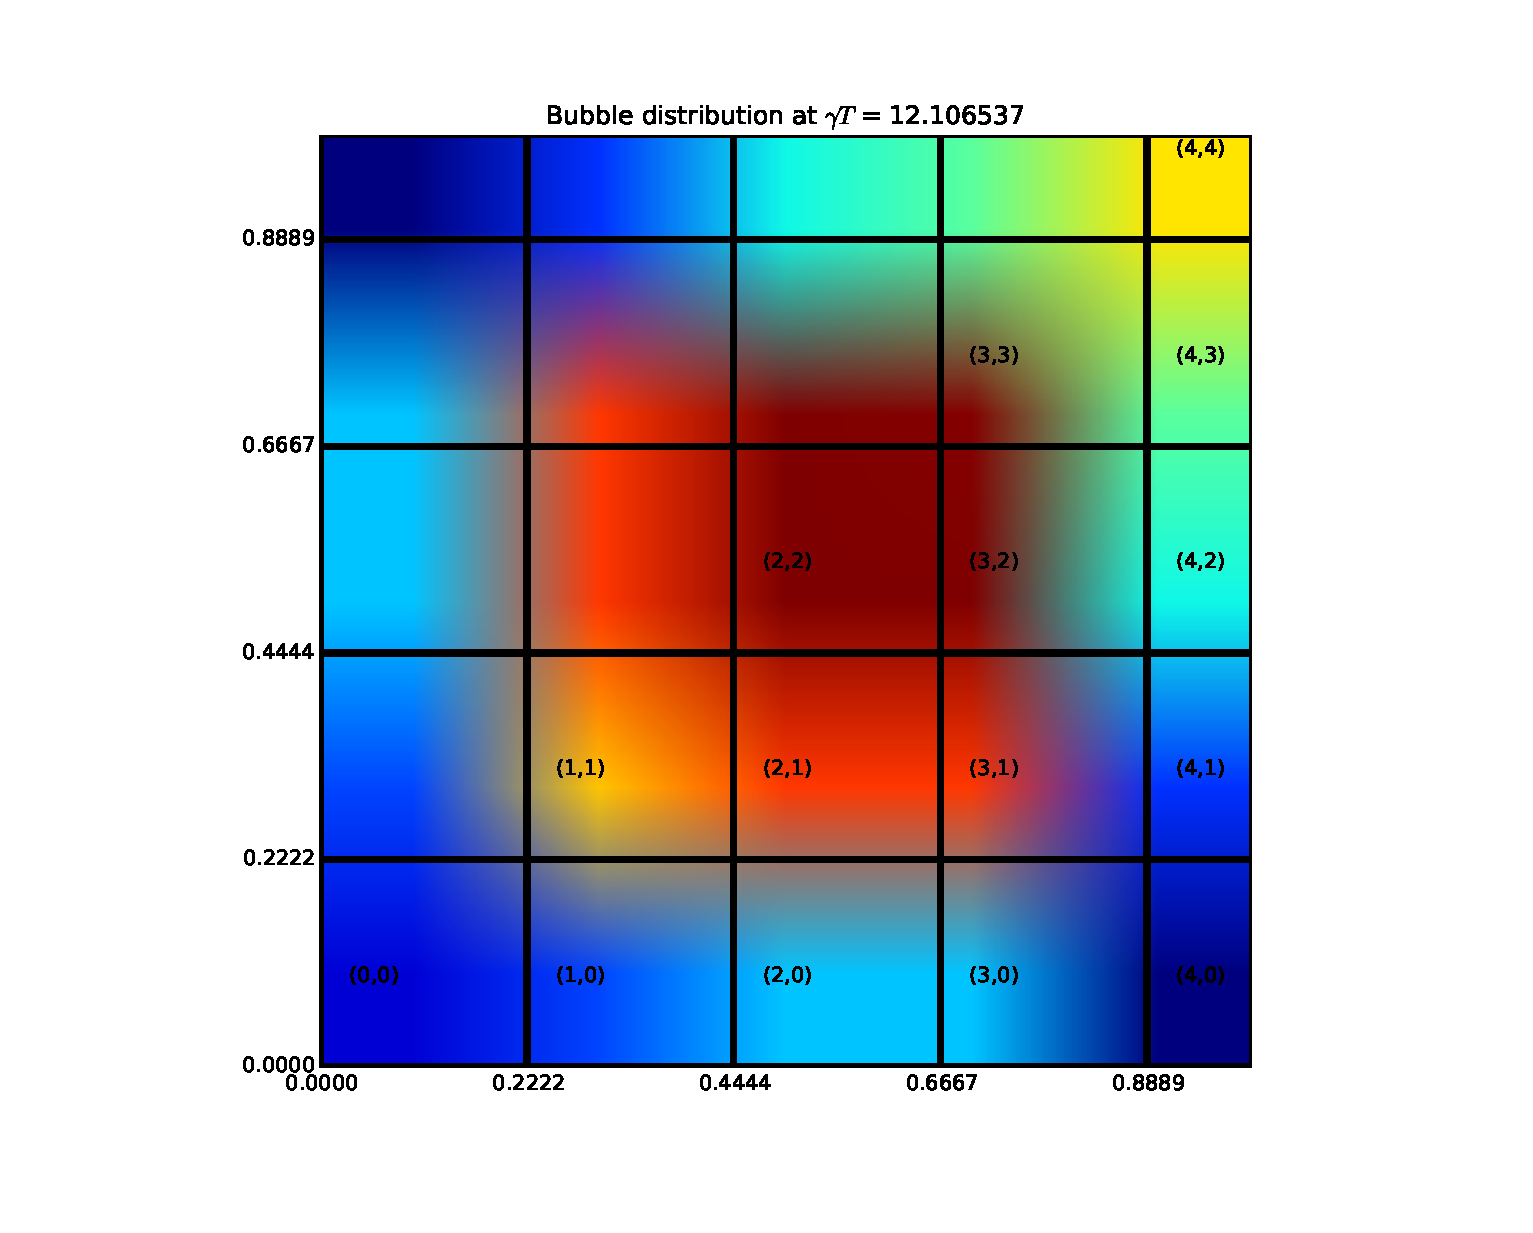
\includegraphics[width=0.66\columnwidth]{figs/spatial_bubble-59}
\end{subfigure}
\caption{ \flabel{bubble_slice}
Spatial distribution of bubble heights at three times.
The first time corresponds to the minimum in \fref{ratio_wall}, which is during the transition from linear to non-linear growth
The second time is taken from the stagnation phase.
The third time is taken from the end of the simulation when the central bubbles are squeezed by the growing boundary layer.
}
\end{figure*}

The individual bubble heights for the $4.5$ mode case are computed as in \eref{h_exp}, but restricted to the span-wise domain nearest to the bubble tip, which is marked in \fref{ic}.
The bubble Froude numbers are plotted in \fref{froude_wall}, alongside the aggregate and purely periodic values.

There are at least three mechanisms by which the walls divert the flow from its fully-periodic preference.
The first is that the no-slip boundaries that pass along the diagonal of the boundary bubbles and spikes create a boundary layer that viscously damps vertical flow.
The second is that the pressure gradient from the boundary layer pushes the boundary bubbles and spikes towards the interior of the domain.
These two effects have been studied independently in the context of multi-phase bubbles rising near walls~\cite{Takemura2002}, and are characterized as wall drag and lift forces.
Finally, the finite nature of the span-wise lattice of bubbles and spikes, coupled with the vertical symmetry condition that the total bubble volume must equal the total spike volume, breaks one of the 4-fold symmetries of the infinite cubic lattice causing a local aggregation of spikes in the $(0,0)$ corner and of bubbles in the $(4,4)$ corner.
The local aggregation sets up one low-amplitude long-wavelength mode across the diagonal.

These three mechanisms promote and penalize the growth of different bubbles in the finite lattice, allowing us to infer the relative magnitudes of the effects based on the performance of the bubbles compared to their periodic counterparts.
The wall drag penalizes the growth of bubbles that contain a boundary: the bubbles in the 4th column.
Because the effect also penalizes the growth of the spikes that contain boundaries, it should encourage the growth of the bubbles adjacent to those spikes: those in the 0th row.
The effect should alternate and diminish towards the interior of the domain.
The wall lift pushes bubbles and spikes at the boundary towards the interior.
This reduces the form drag on the interior bubbles by increasing the pressure on their trailing edges.
When adjacent bubbles actually touch, skin drag is also reduced.
Overall, wall lift promotes the growth of the interior bubbles.
Finally, the long-wavelength mode promotes growth of bubbles in the bubble heavy corner and penalizes growth of bubbles in the spike heavy corner.

The spatial distribution of the bubble heights can be seen in \fref{bubble_slice} and the heights relative to the periodic bubble can be seen in \fref{ratio_wall}.
At moderate times, the $(4,4)$ bubble leads and the $(0,0)$ bubble trails, indicating that the long-wavelength mode due to symmetry breaking is the dominant effect.
Additionally, all of the bubbles under-perform their periodic counterpart, indicating that the wall drag has damped the overall flow but with less spatial dependence than the long-wavelength mode.
At late times, the central $(2,2)$, $(2,1)$  bubbles are accelerated while the edge bubbles break down, indicating the growing importance of the wall lift effect.
The wall lift ultimately leads to bubble collisions that destroy the bubble lattice, enhance mixing, and break down the flow.

\subsubsection{Late-time behavior}

\begin{figure*}
\begin{subfigure}[b]{\columnwidth}
  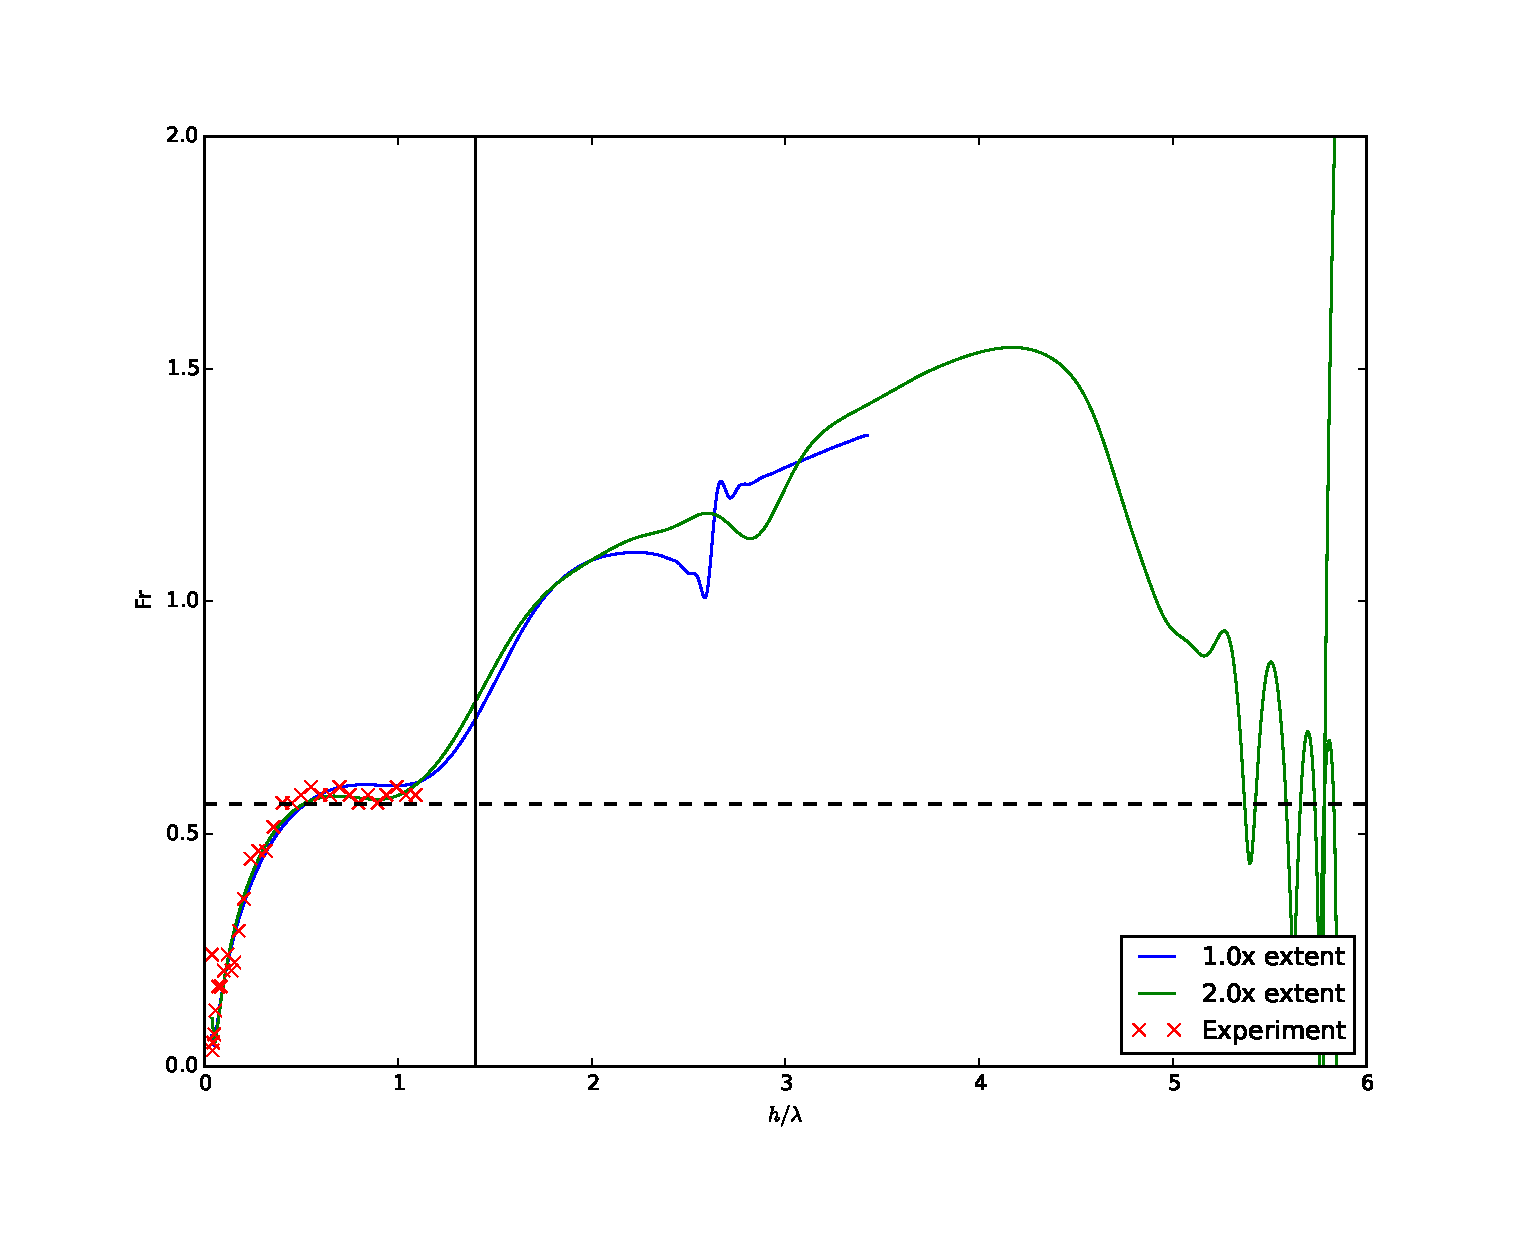
\includegraphics[width=\columnwidth]{plts/Fr_long}
\end{subfigure}
\begin{subfigure}[b]{\columnwidth}
  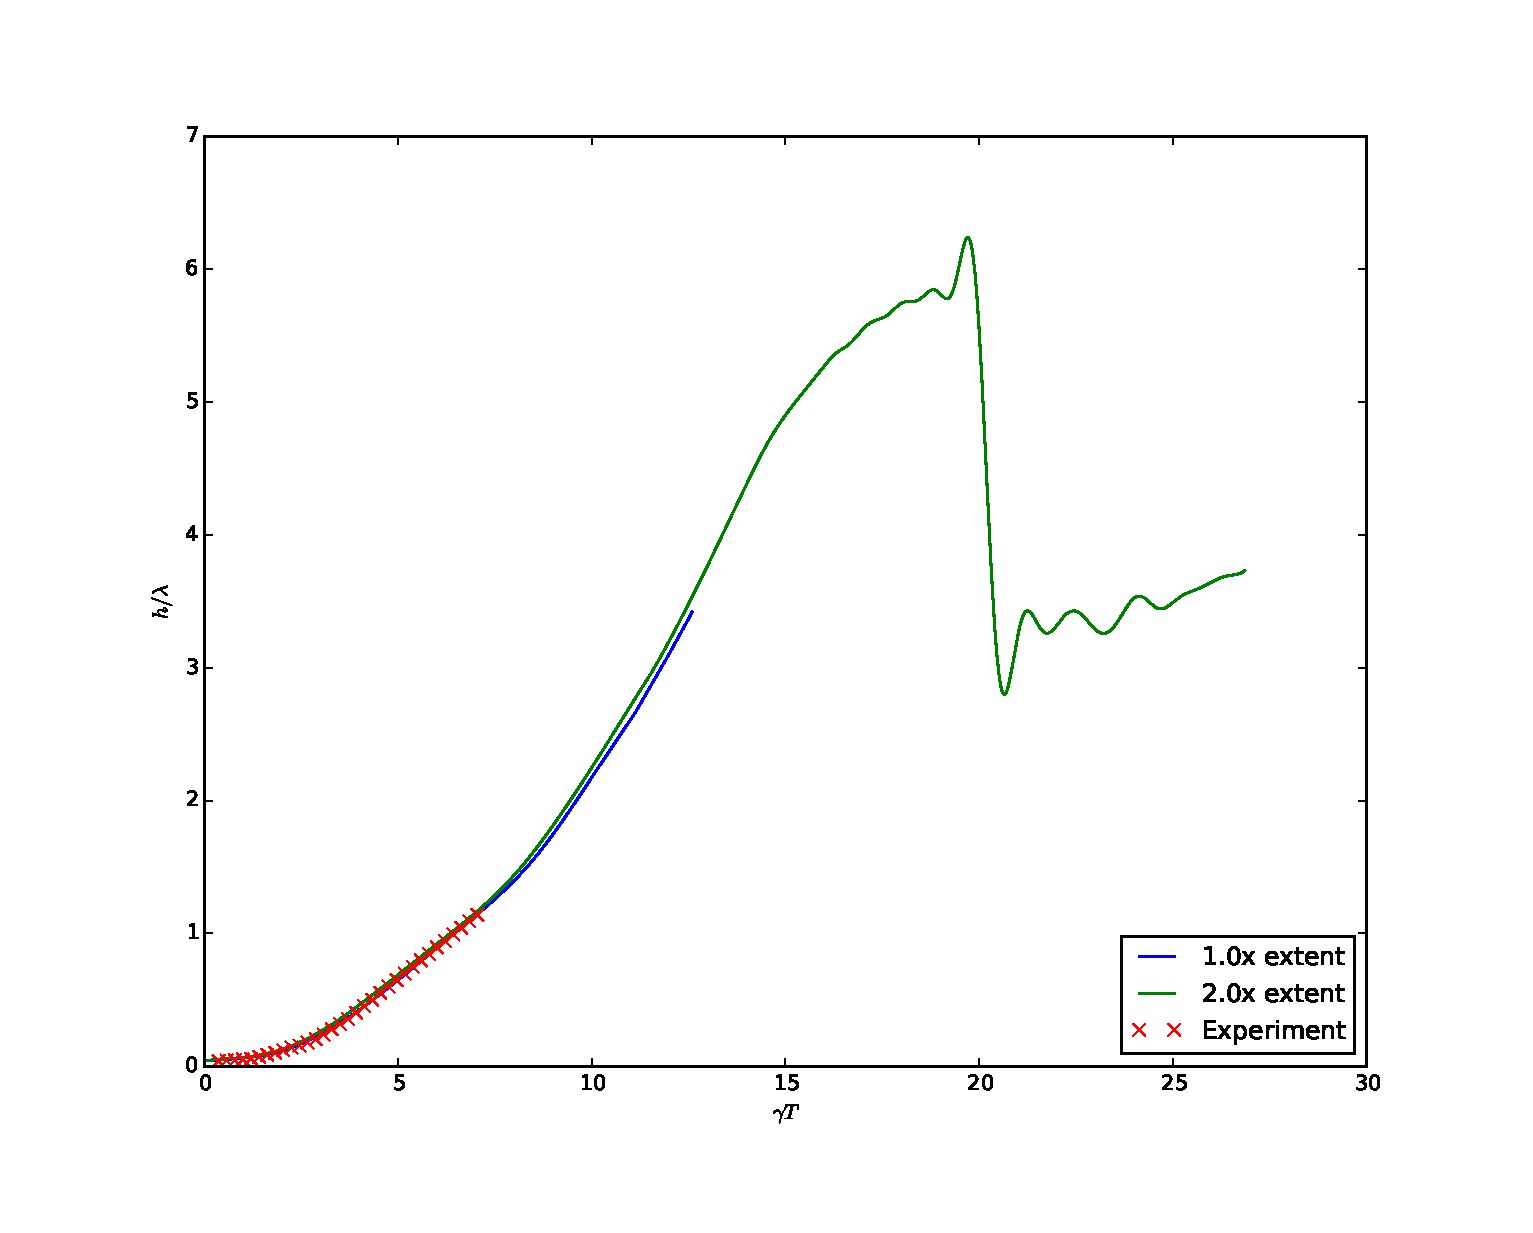
\includegraphics[width=\columnwidth]{plts/aspect_long}
\end{subfigure}
\caption{ \flabel{long_dynamics}
Bubble velocity and bubble height vs time, non-dimensionalized by the wavelength and linear growth rate, for 4.5 mode simulations and experiment.
Lines are from simulation output, one case with the same vertical extent as the simulation and in the other with twice that vertical extent.
Points are from experiment via direct measurement of the bubble velocity and bubble height.
The dotted horizontal line is positioned at Goncharov's theoretical value of $\pi^{-1/2}$~\cite{Goncharov2002}.
The solid vertical line marks the greatest bubble height reached in any of the experiments by Wilkinson and Jacobs~\cite{Wilkinson2007}.
}
\end{figure*}

\begin{figure*}
\begin{subfigure}[b]{0.66\columnwidth}
  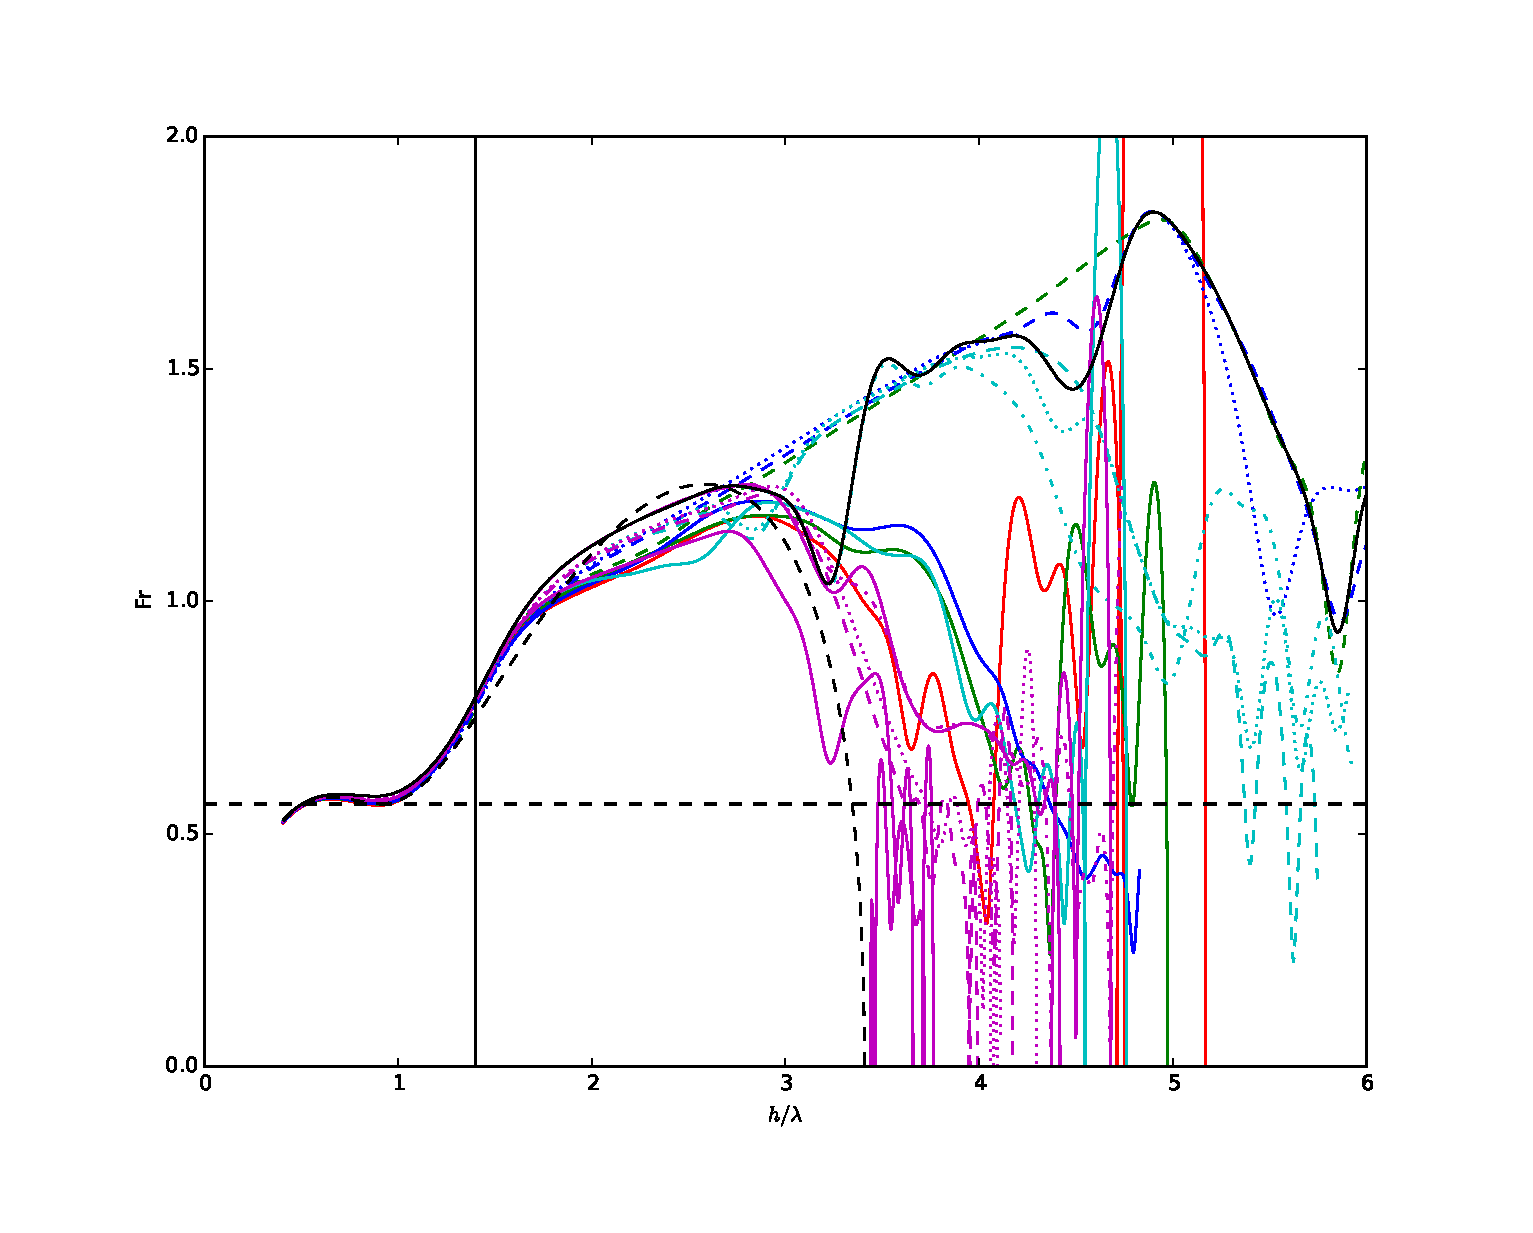
\includegraphics[width=0.66\columnwidth]{plts/Fr_long_walls}
\end{subfigure}
\begin{subfigure}[b]{0.66\columnwidth}
  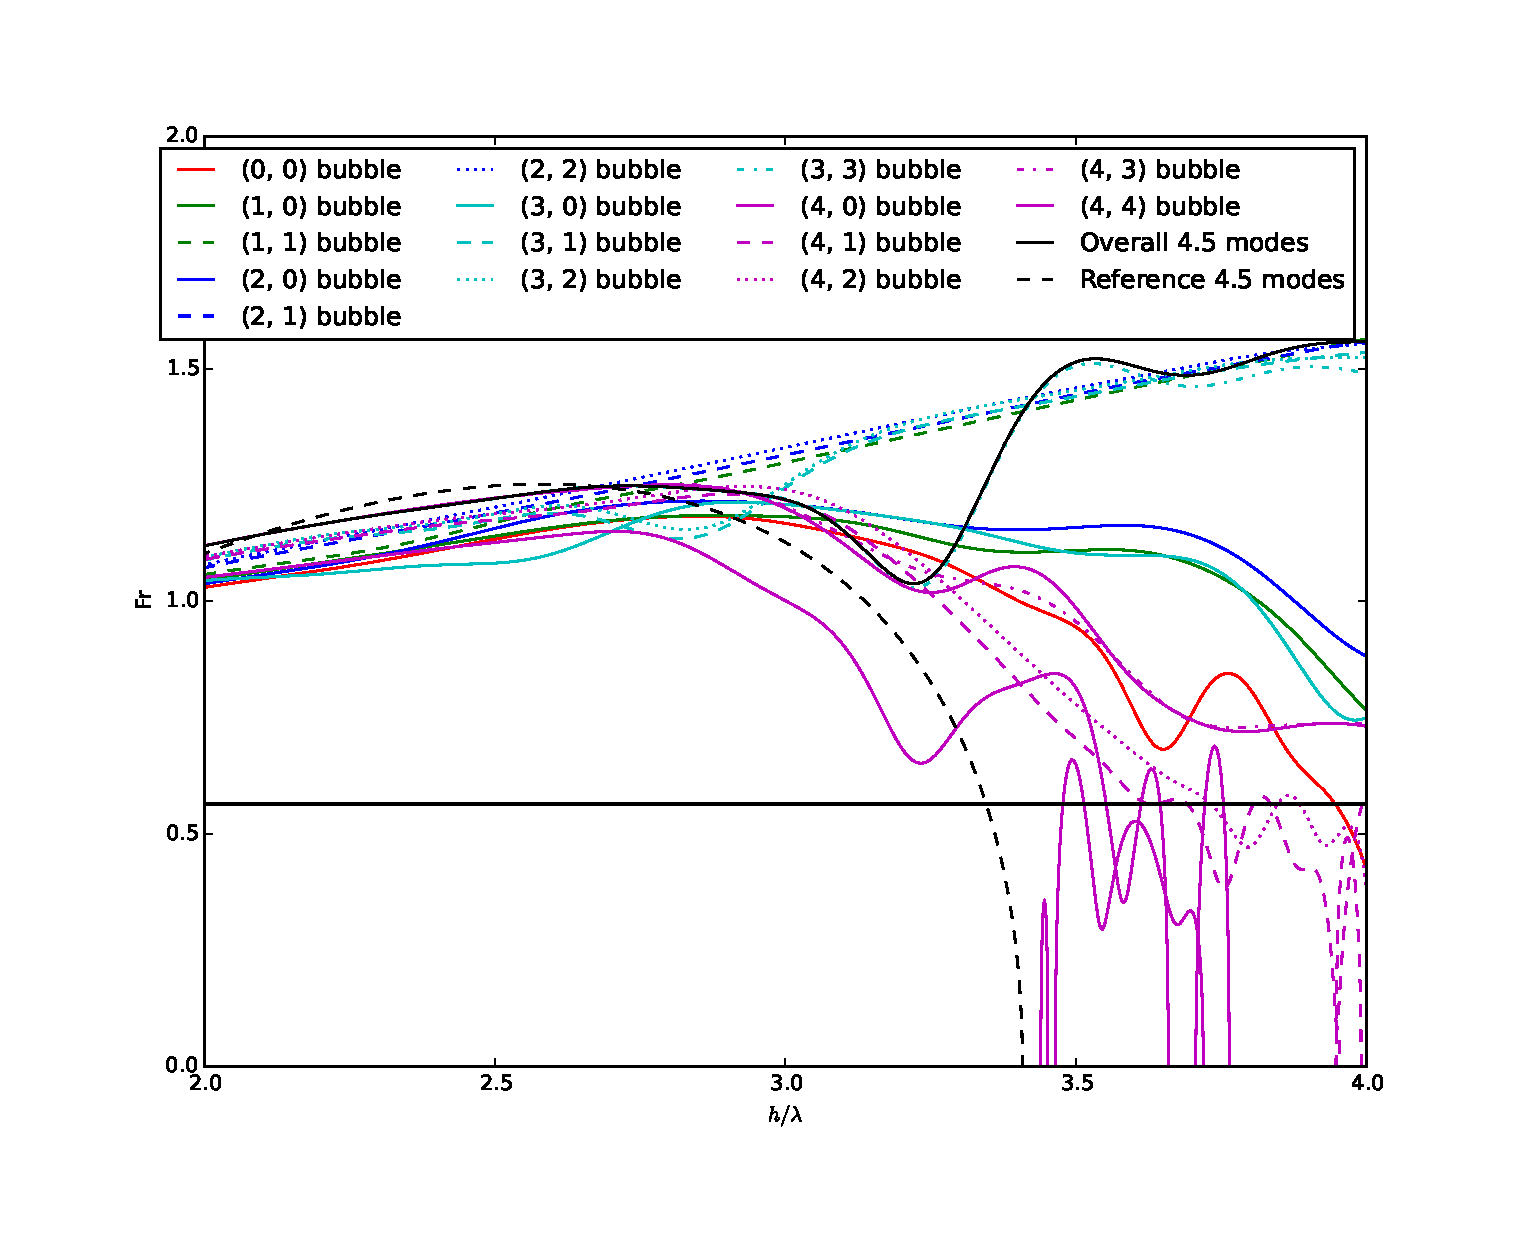
\includegraphics[width=0.66\columnwidth]{plts/Fr_long_walls_zoom1}
\end{subfigure}
\begin{subfigure}[b]{0.66\columnwidth}
  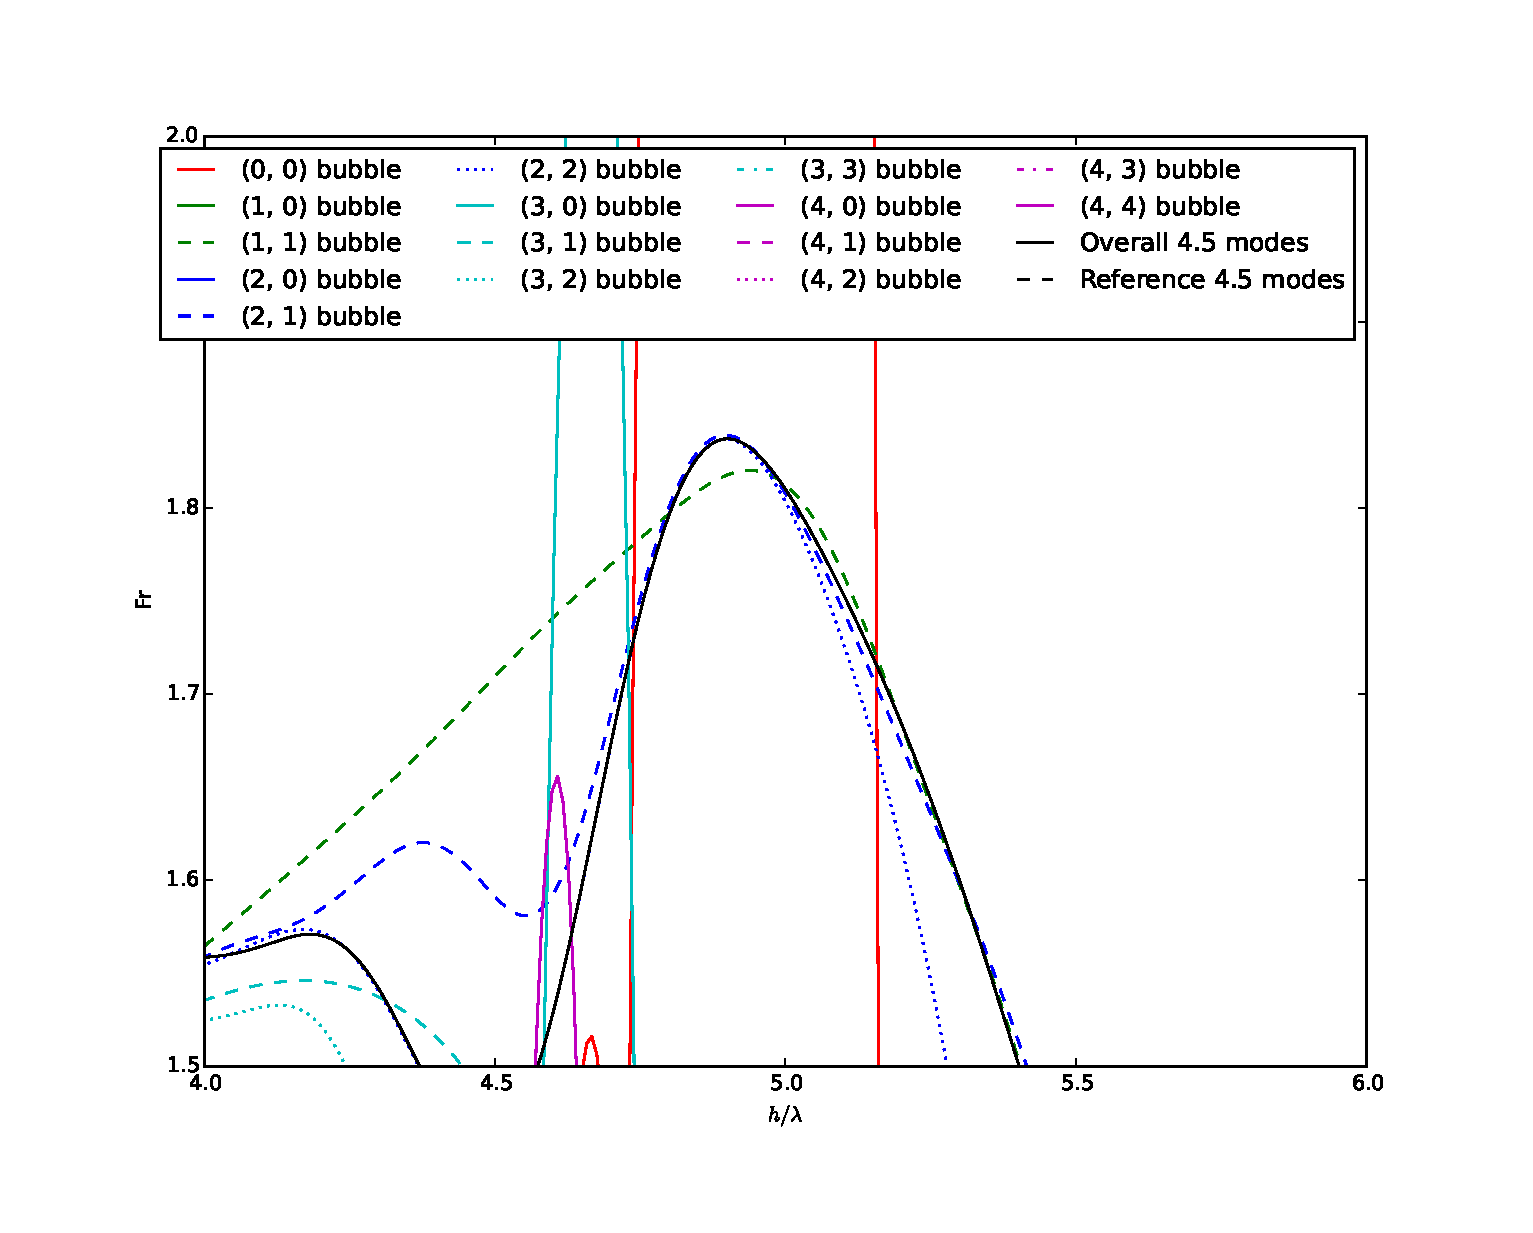
\includegraphics[width=0.66\columnwidth]{plts/Fr_long_walls_zoom2}
\end{subfigure}
\caption{ \flabel{long_wall_dynamics}
Froude number as a function of height, non-dimensionalized by the wavelength, by bubble in the 4.5 mode simulation with extended vertical extent.
Solid line is from the height defined as the maximum taken over the entire span-wise domain.
Dotted line is the periodic reference calculation.
The dotted horizontal line is positioned at Goncharov's theoretical value of $\pi^{-1/2}$~\cite{Goncharov2002}.
The solid vertical line marks the greatest bubble height reached in any of the experiments by Wilkinson and Jacobs~\cite{Wilkinson2007}.
}
\end{figure*}


The 4.5 mode simulation was repeated with twice the vertical extent and simulation time.
Additionally, the Schmidt number was increased from 1 to 3.5 to reduce late-time mixing not present in high Schmidt number experiments.
\fref{long_dynamics} compares the short unit-Schmidt and long moderate-Schmidt trajectories, which are widely in agreement.
The reduction in bubble acceleration around aspect ratio $h/\lambda = 2$ is present in both the short and the long simulations, so it is unlikely to be due to the vertical domain boundaries.
It is not, however, present in the periodic calculation, so it could be a wall effect.

\fref{long_wall_dynamics} mimics \fref{froude_wall} but for the late-time case.
The periodic reference trajectory, calculated with the original domain size, rapidly decays after reaching a maximum around aspect ratio $h/\lambda = 2.5$ due to interactions with the top of the domain.
Its maximum Froude number is around 1.2, consistent with previous calculations.
The central bubbles in the extended late-time run continue to experience constant acceleration past aspect ratio 3 and Froude number 1.2, with the $(1,1)$ bubble continuing to aspect ratio 5 and Froude number 1.8.

The decay of the velocity of the periodic reference bubble around $h/\lambda = 2.5$ suggests the late-time simulations would interact with the top boundary around $h/\lambda = 5$.
In fact, this is exactly when the $(1,1)$ and $(2,2)$ bubbles begin to decay.
However, the bubbles closer to the boundaries break down much earlier.
The $(4,4)$ bubble, for example, reaching maximum Froude number around $h/\lambda = 2.75$.
We can infer that the wall lift that drives the boundary bubbles into the interior bubbles destroys the periodic ordering.
It is not clear if the decay of the interior bubbles at $h/\lambda = 5$ is due to the top boundary or the wall lift destroying the periodic ordering.

\subsubsection{Secondary flow}

\begin{figure*}
\begin{subfigure}[b]{0.66\columnwidth}
  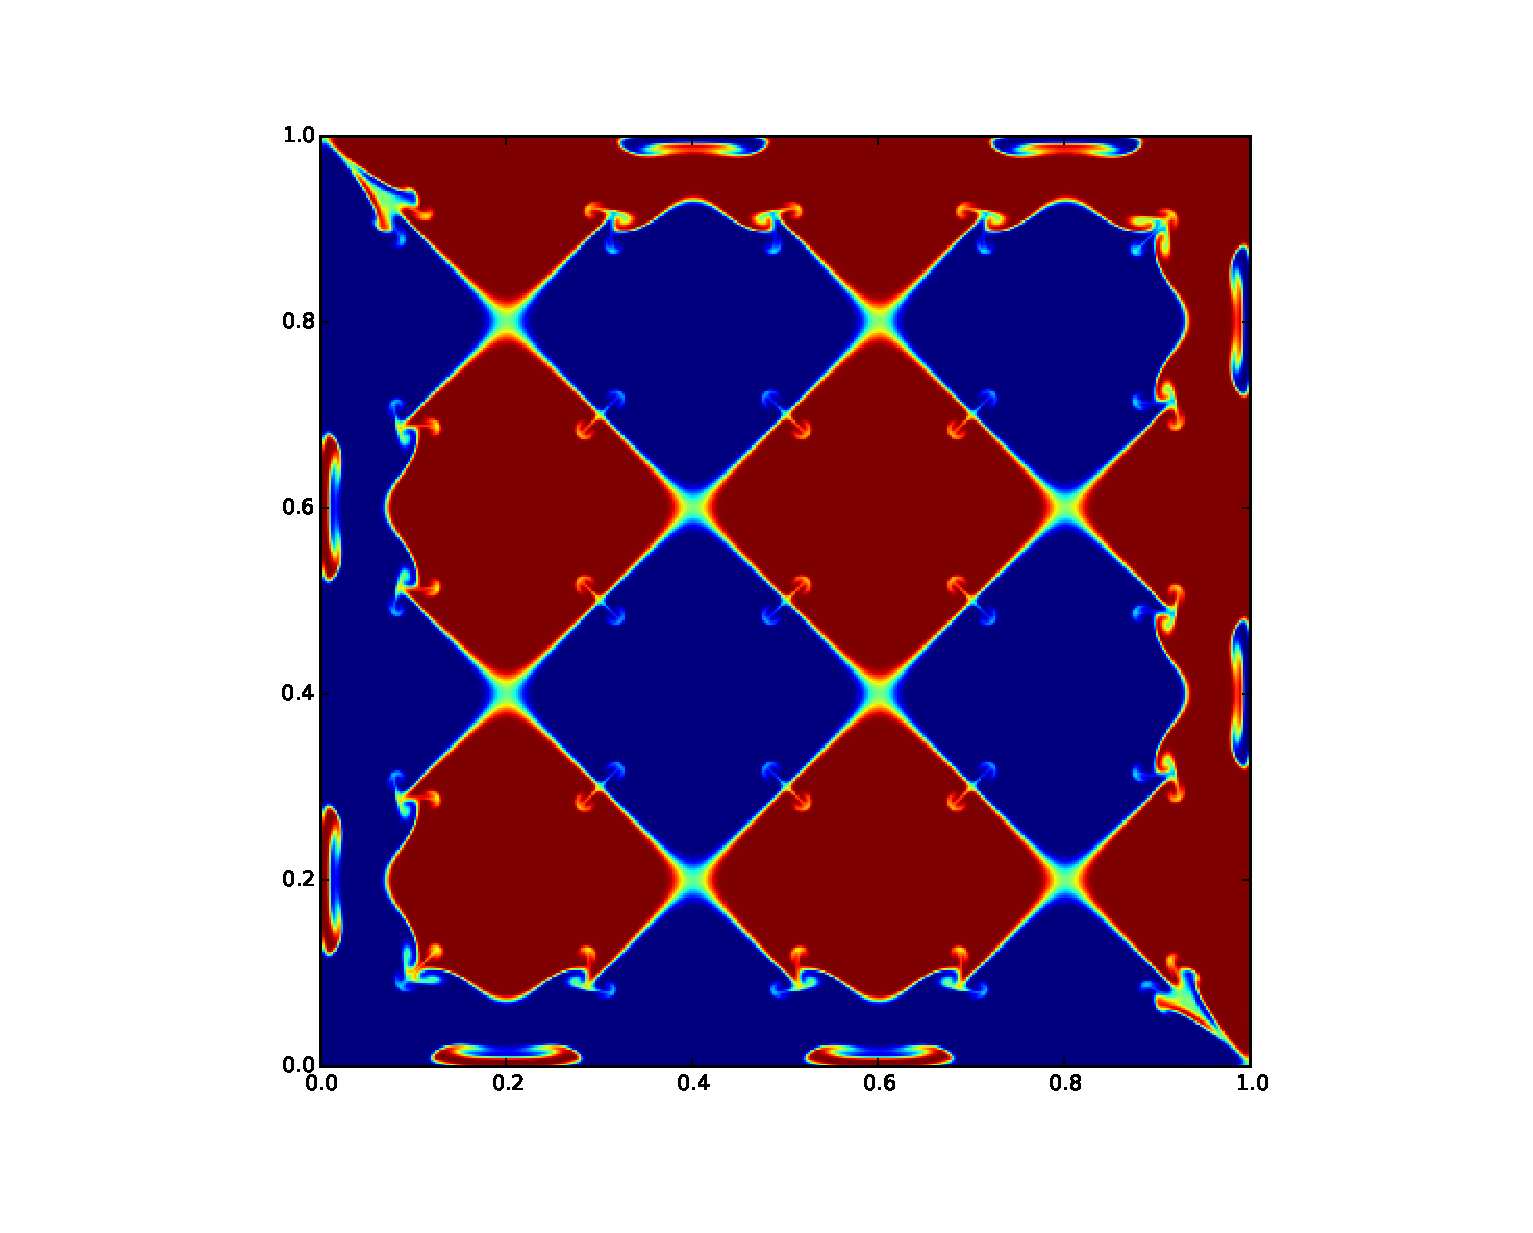
\includegraphics[width=0.66\columnwidth]{figs/scalar-25-20}
\end{subfigure}
\begin{subfigure}[b]{0.66\columnwidth}
  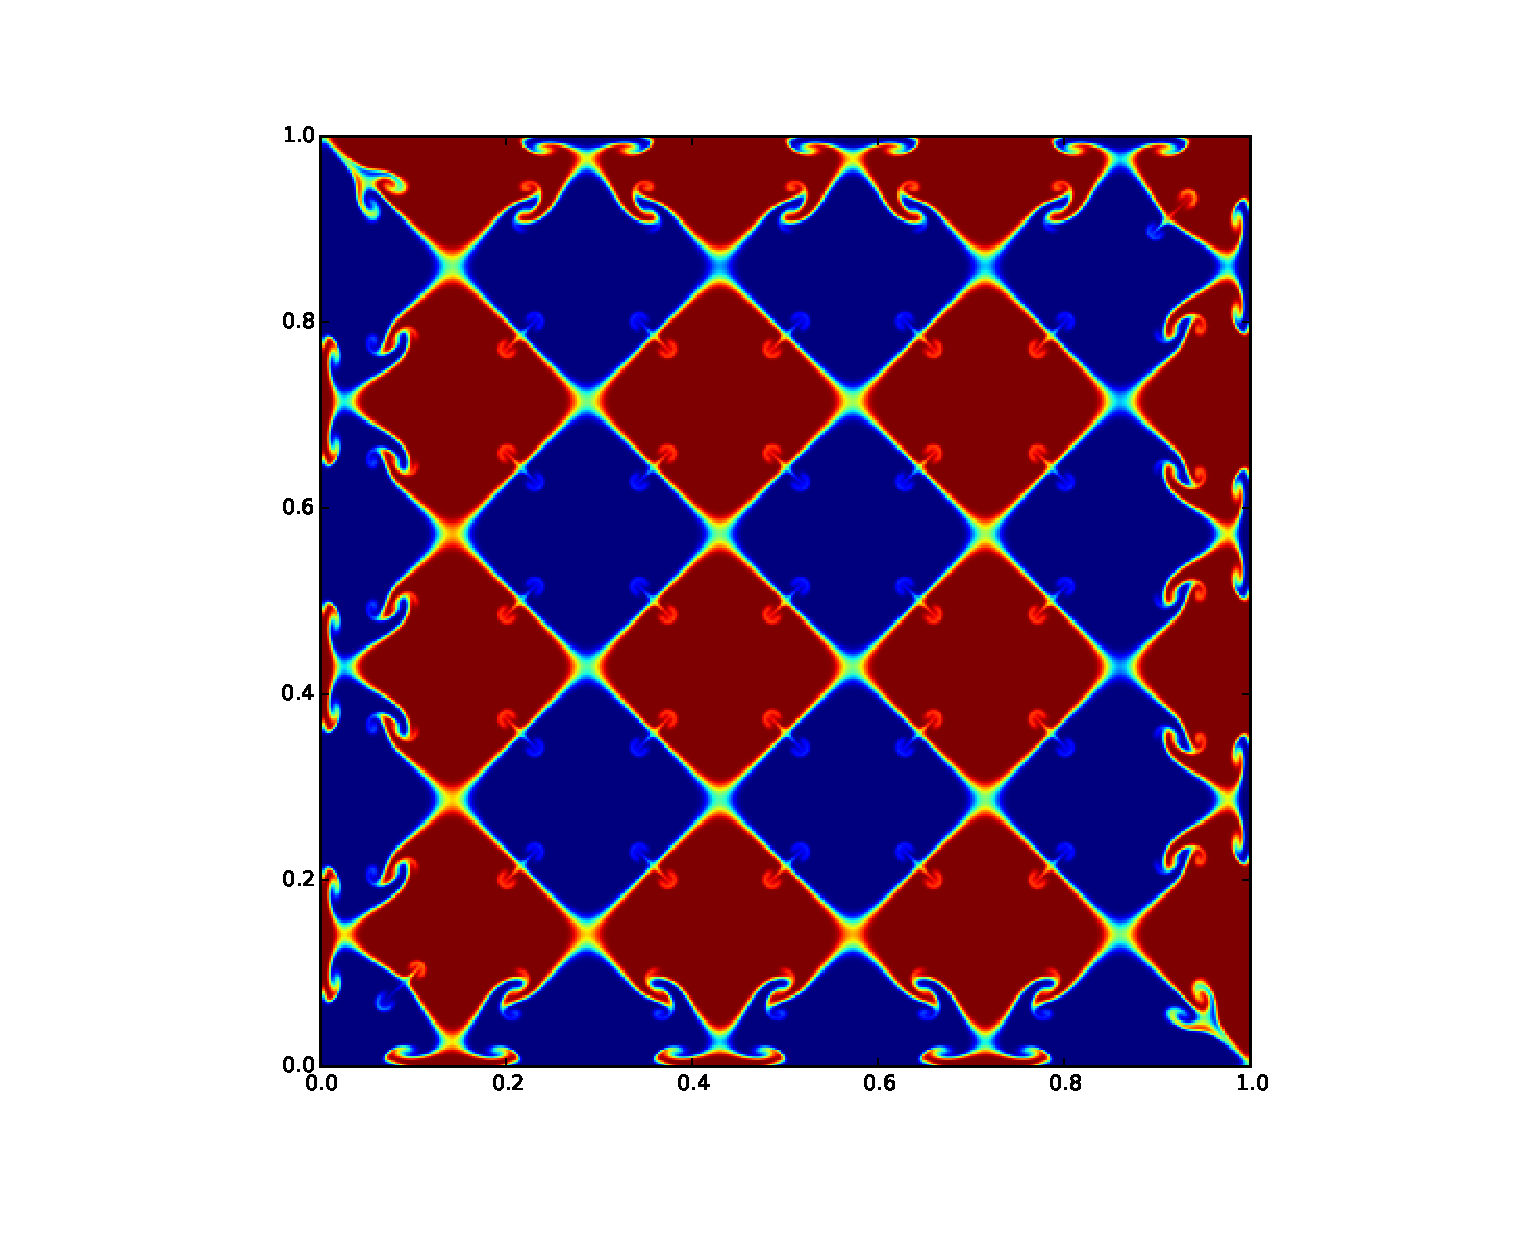
\includegraphics[width=0.66\columnwidth]{figs/scalar-35-20}
\end{subfigure}
\begin{subfigure}[b]{0.66\columnwidth}
  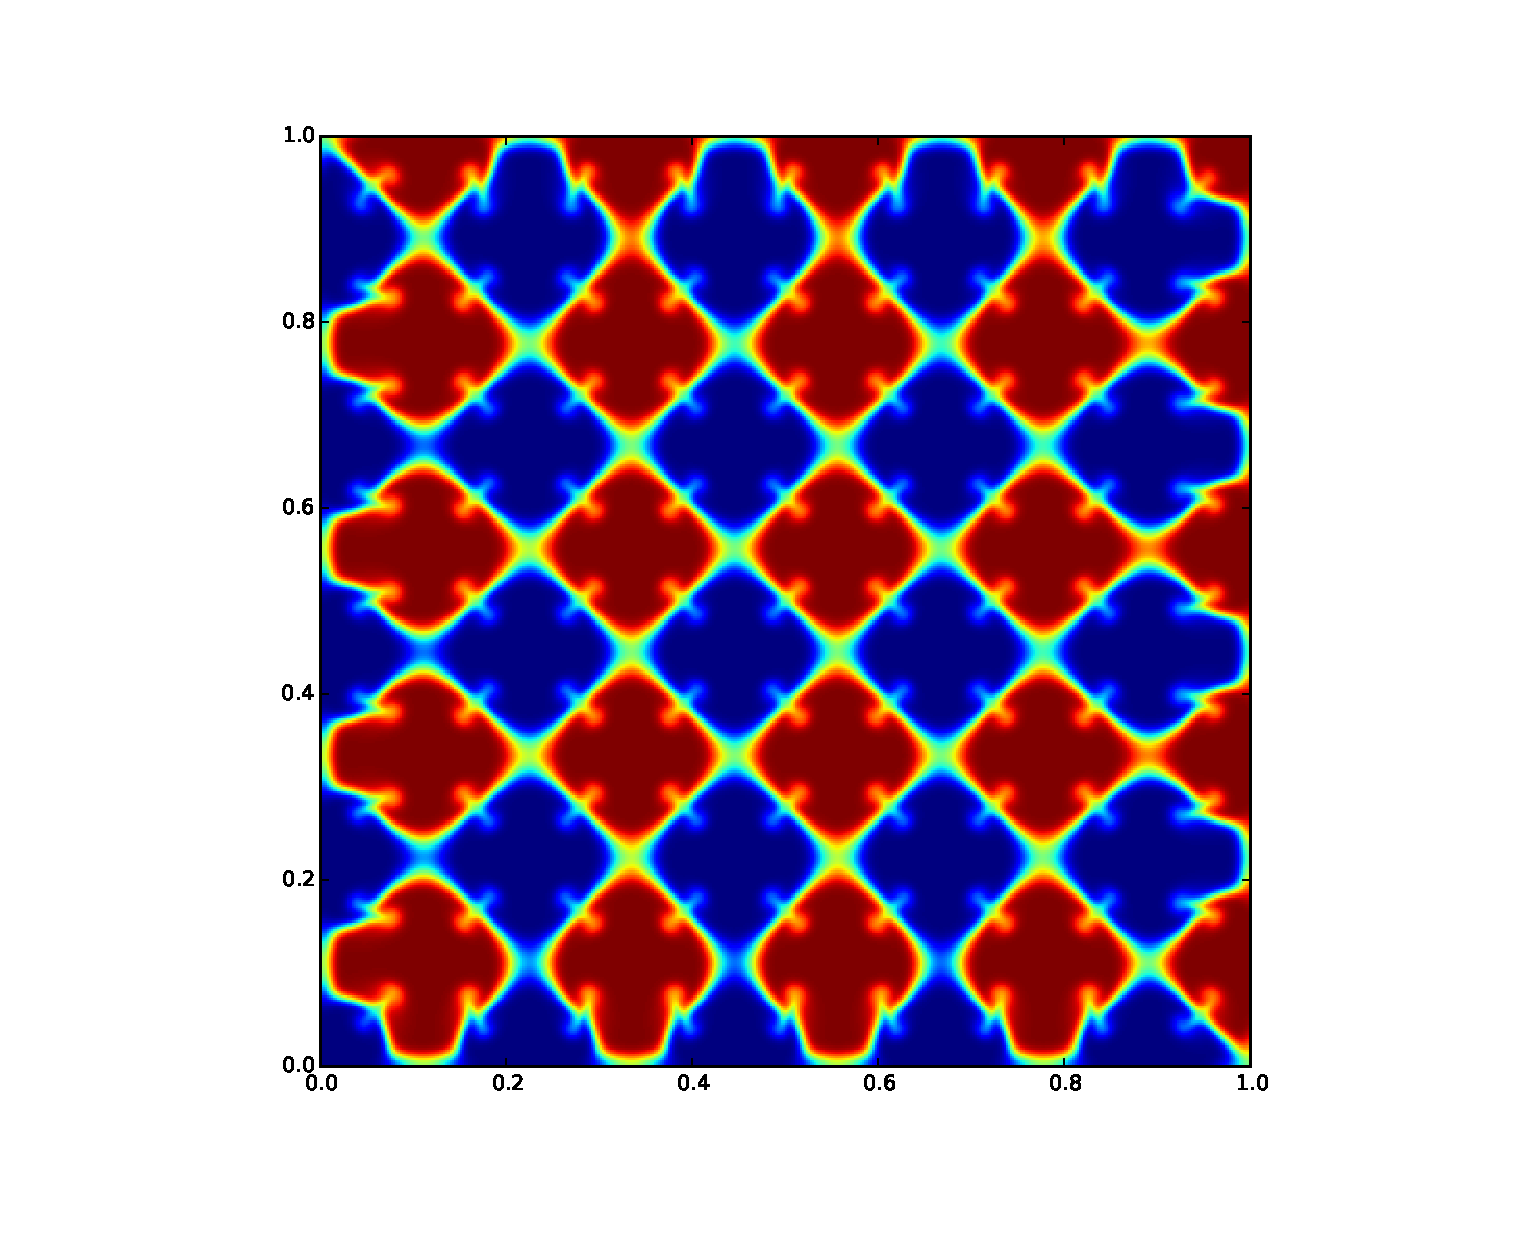
\includegraphics[width=0.66\columnwidth]{figs/scalar-45-20}
\end{subfigure}
\caption{ \flabel{phixy}
Scalar field in the horizontal mid-plane for 2.5, 3.5, and 4.5 mode simulations.
}
\end{figure*}



\begin{figure*}
\begin{subfigure}[b]{0.66\columnwidth}
  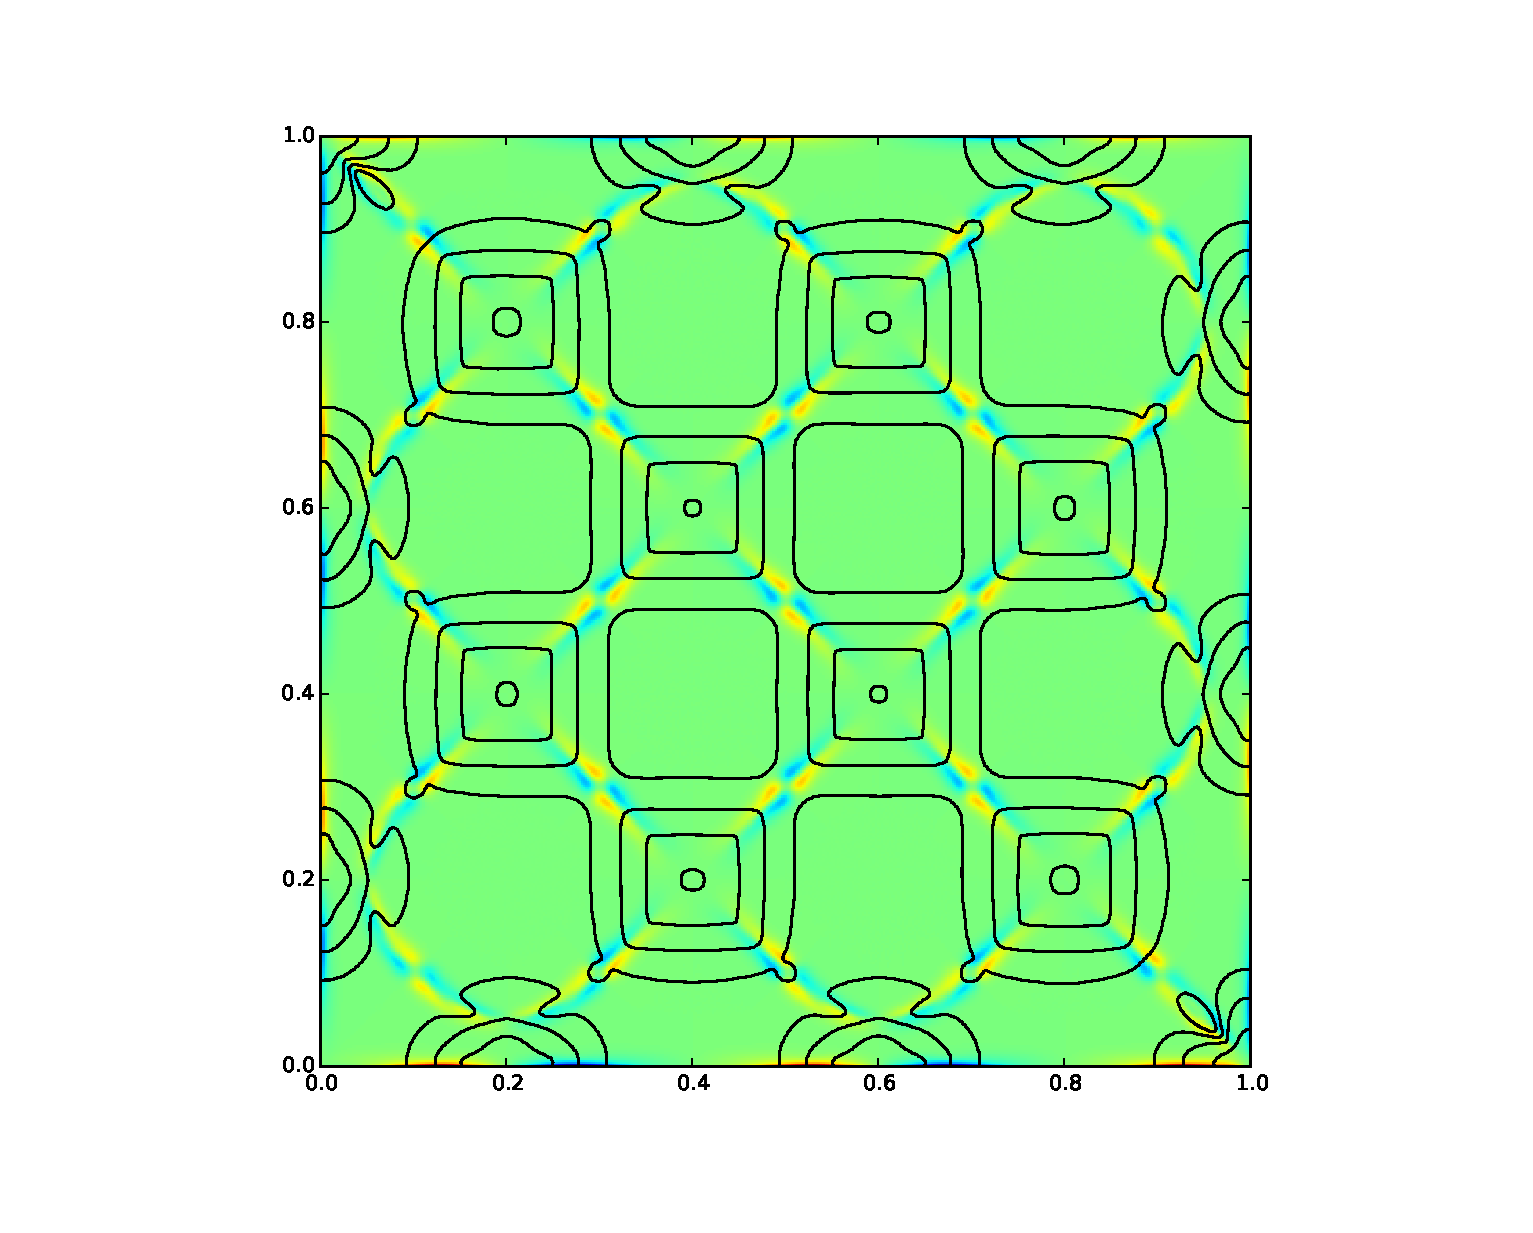
\includegraphics[width=0.66\columnwidth]{figs/vorticity-25-10}
\end{subfigure}
\begin{subfigure}[b]{0.66\columnwidth}
  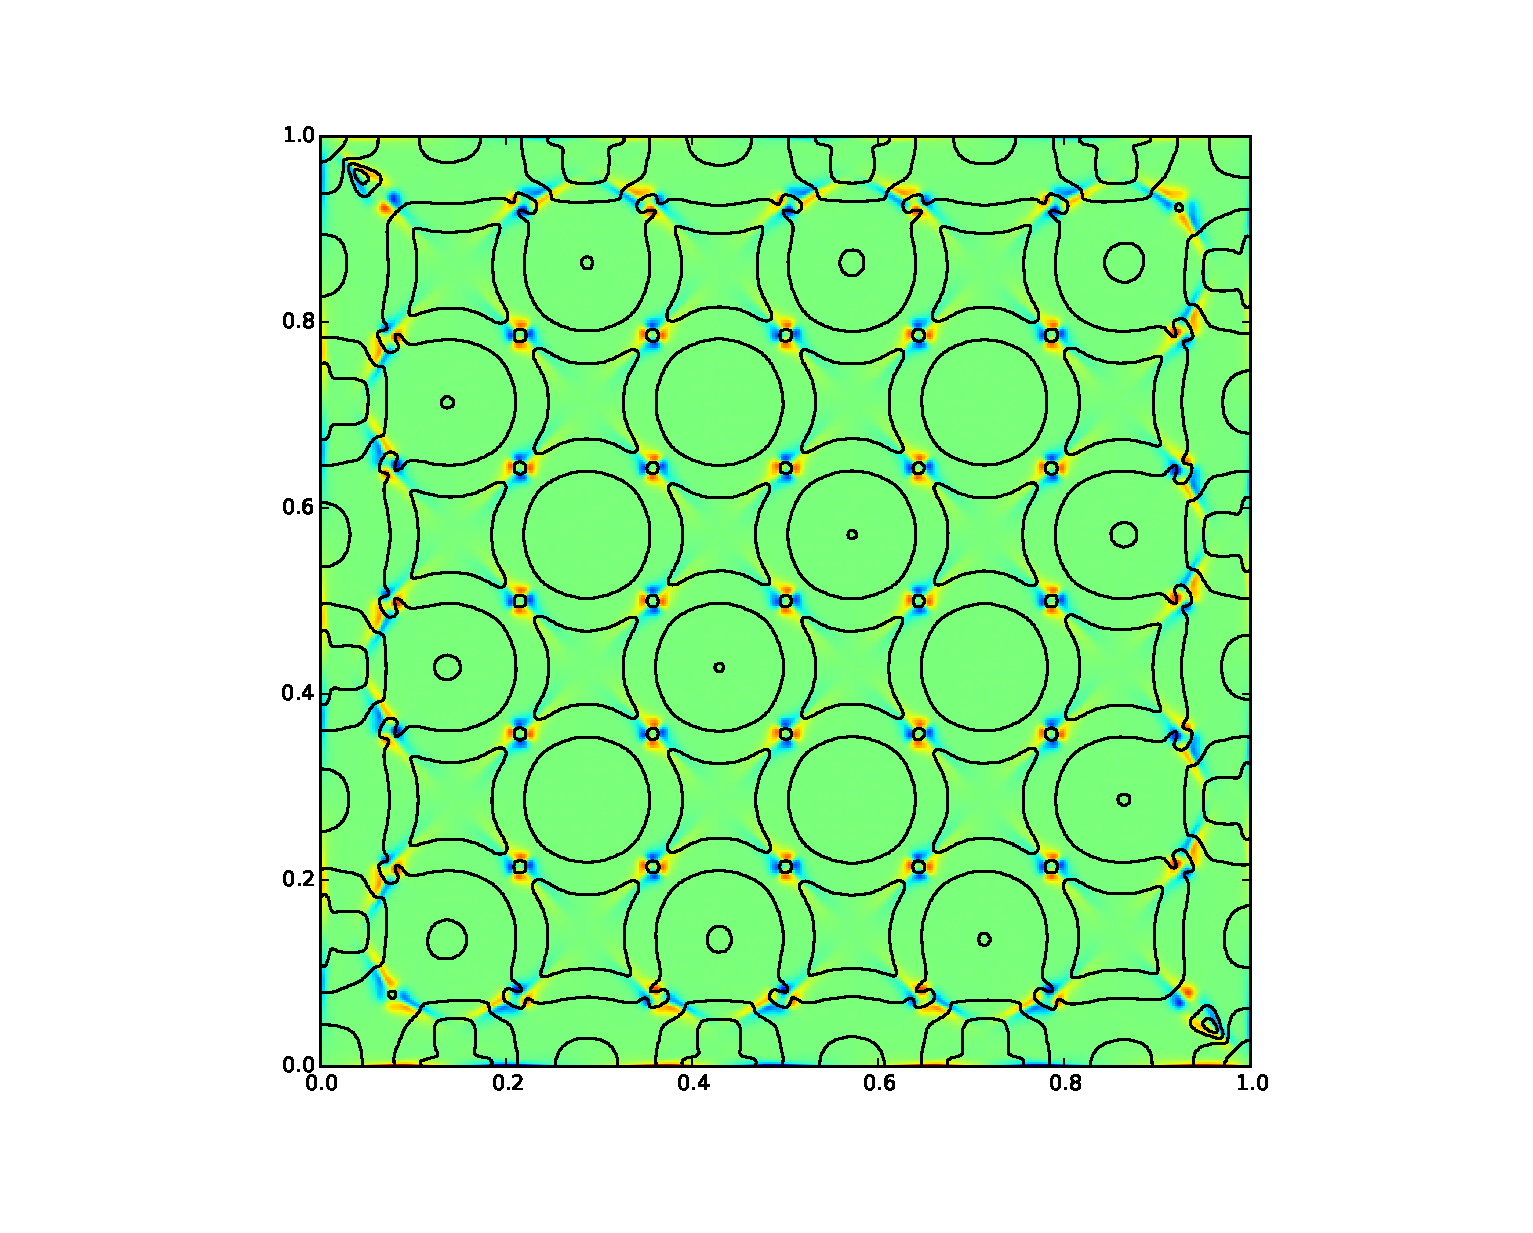
\includegraphics[width=0.66\columnwidth]{figs/vorticity-35-10}
\end{subfigure}
\begin{subfigure}[b]{0.66\columnwidth}
  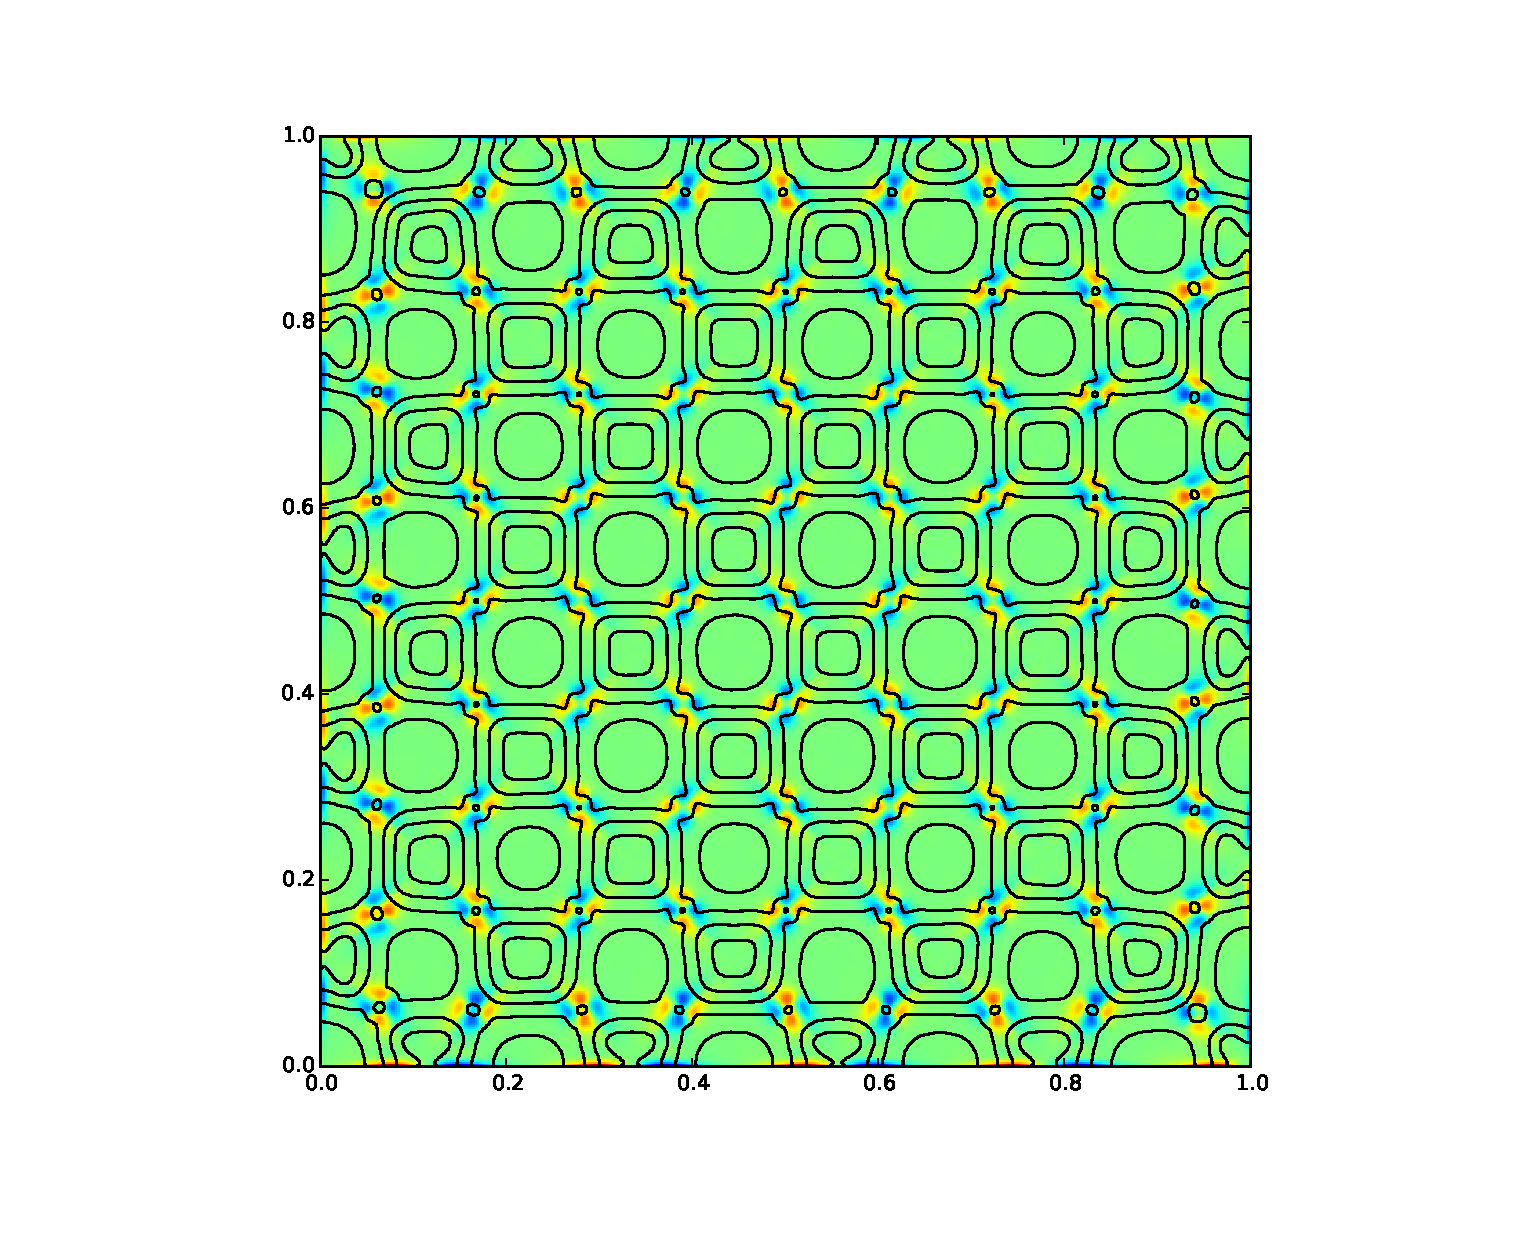
\includegraphics[width=0.66\columnwidth]{figs/vorticity-45-10}
\end{subfigure}
\caption{ \flabel{secondary}
Secondary flow in the horizontal mid-plane.
Background color is the vertical component of the vorticity.
Contours are lines of constant pressure.
}
\end{figure*}

\begin{figure*}
\begin{subfigure}[b]{0.66\columnwidth}
  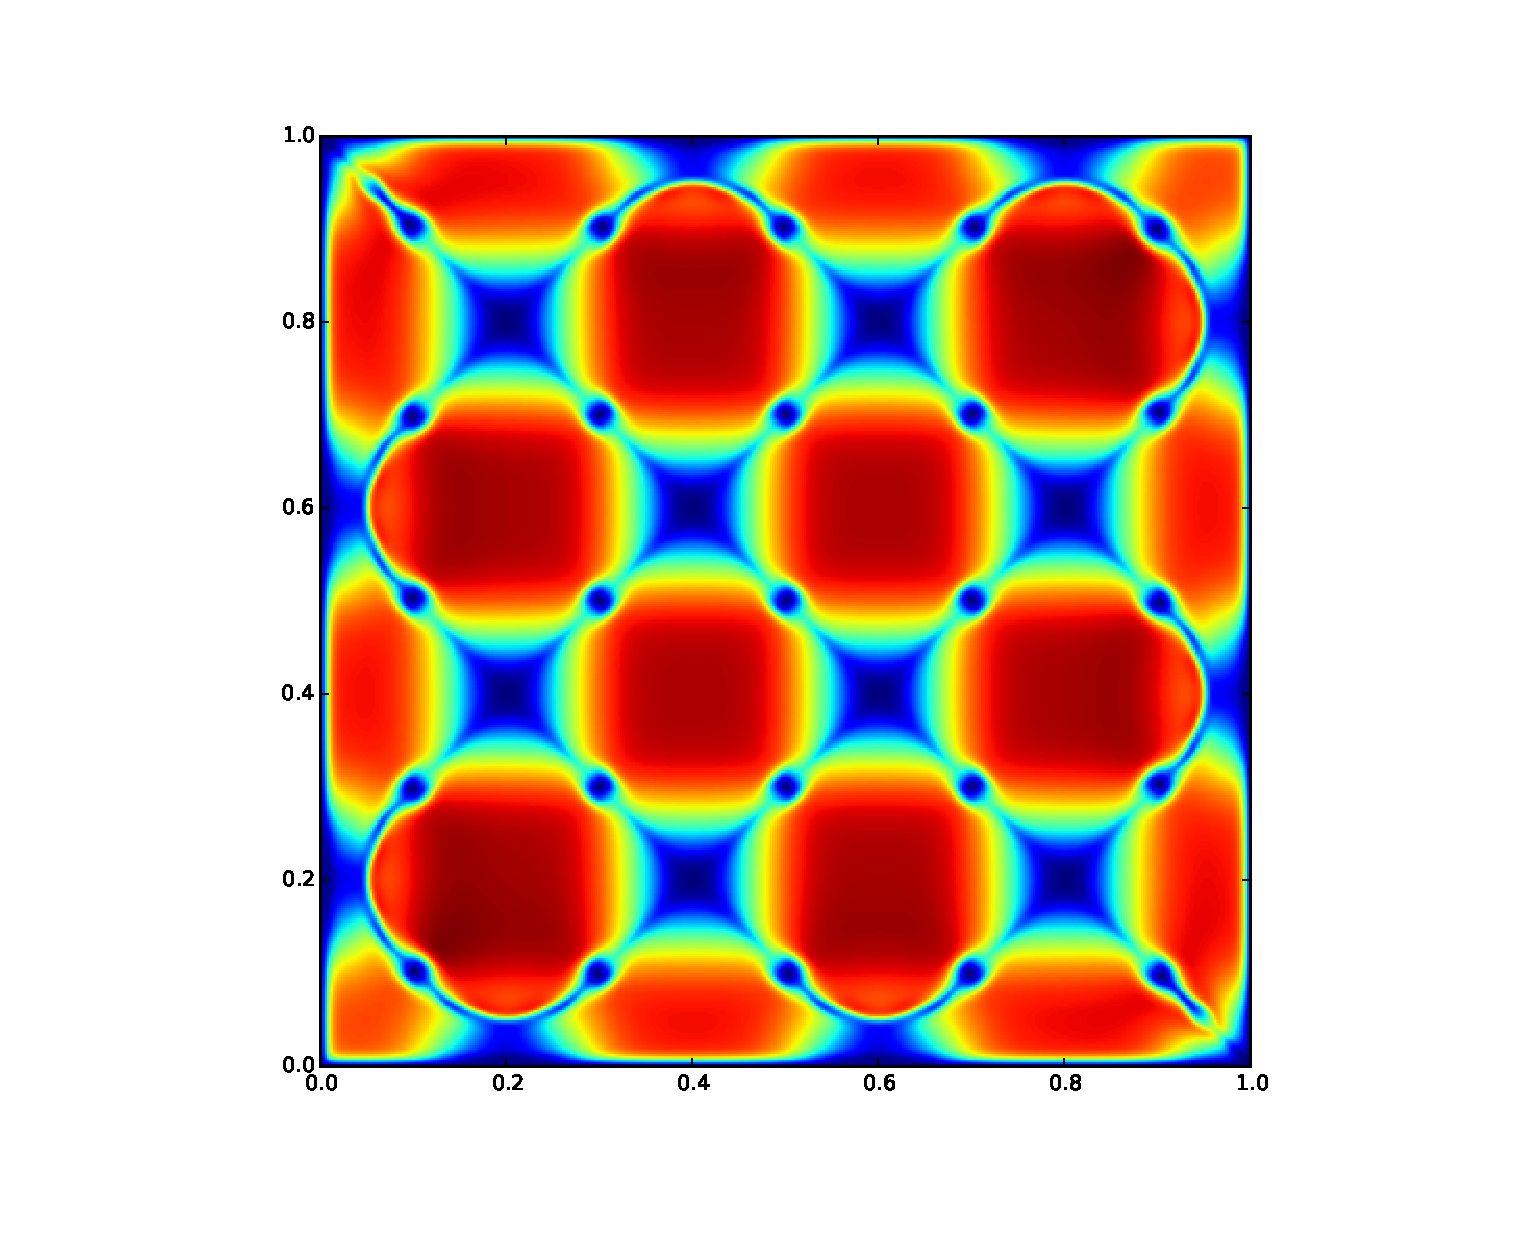
\includegraphics[width=0.66\columnwidth]{figs/dynamic_pressure-25-10}
\end{subfigure}
\begin{subfigure}[b]{0.66\columnwidth}
  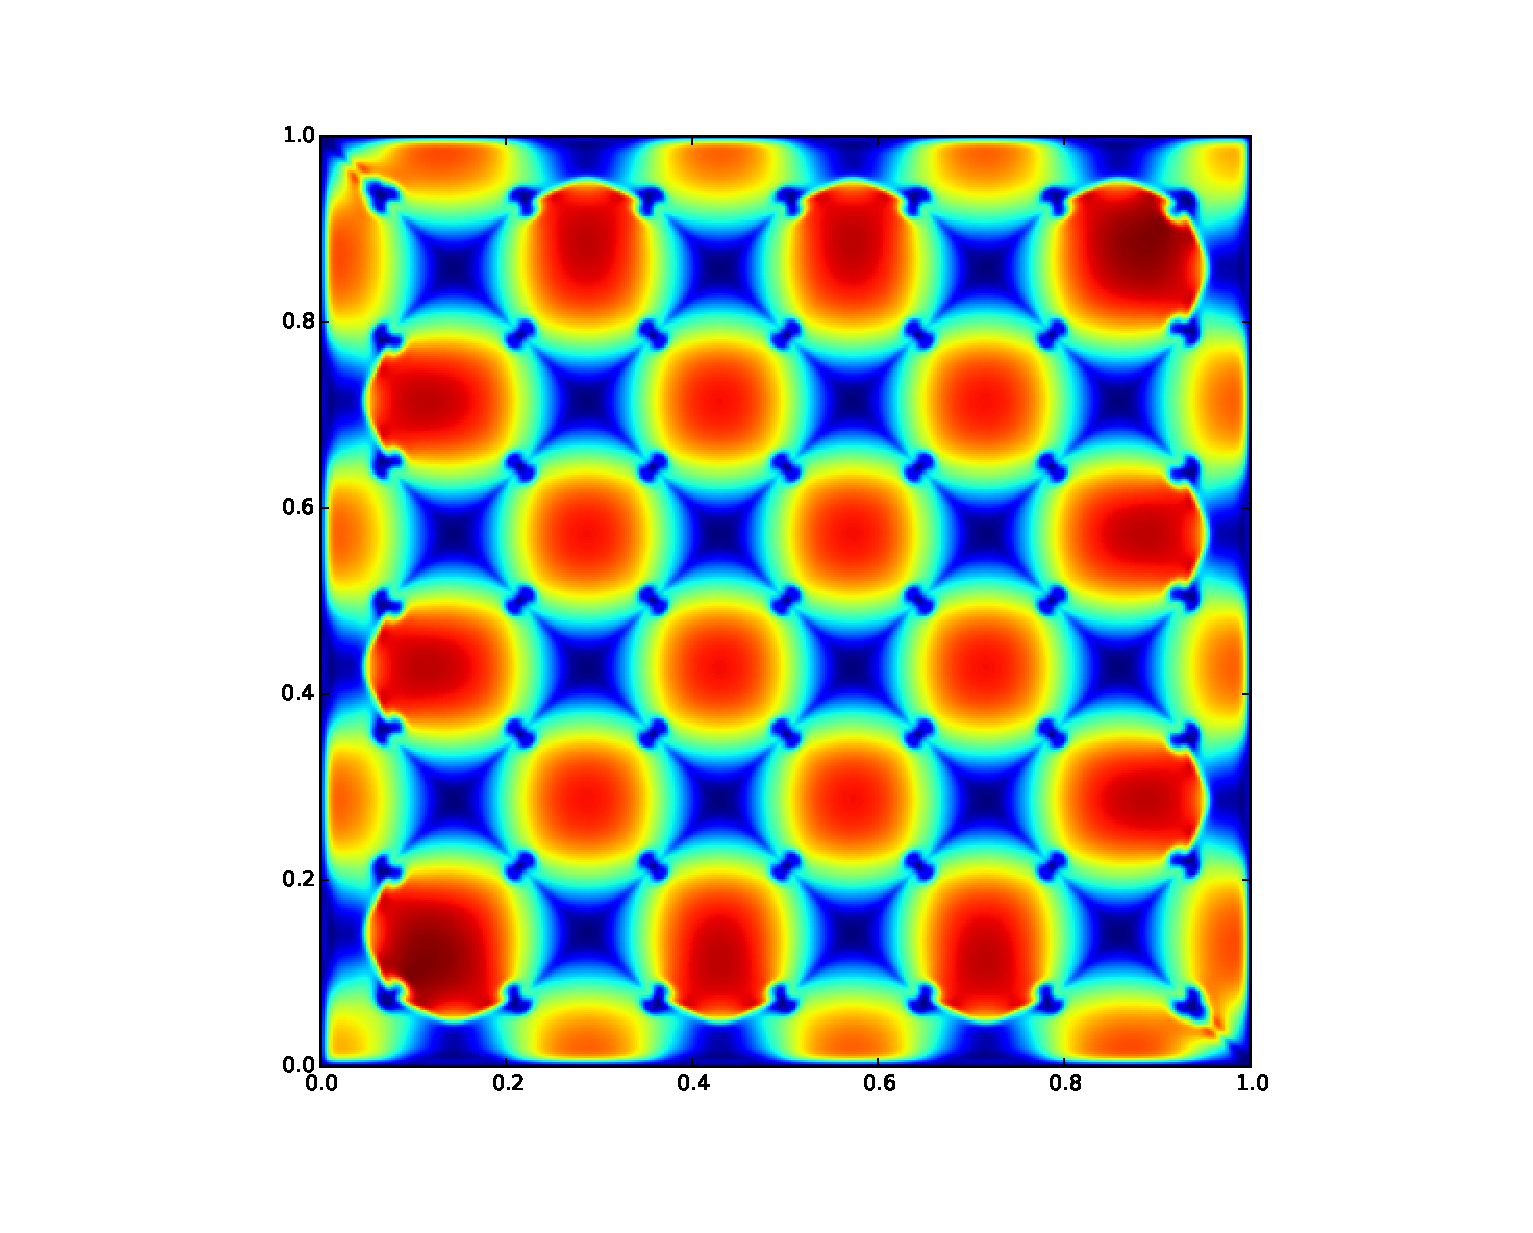
\includegraphics[width=0.66\columnwidth]{figs/dynamic_pressure-35-10}
\end{subfigure}
\begin{subfigure}[b]{0.66\columnwidth}
  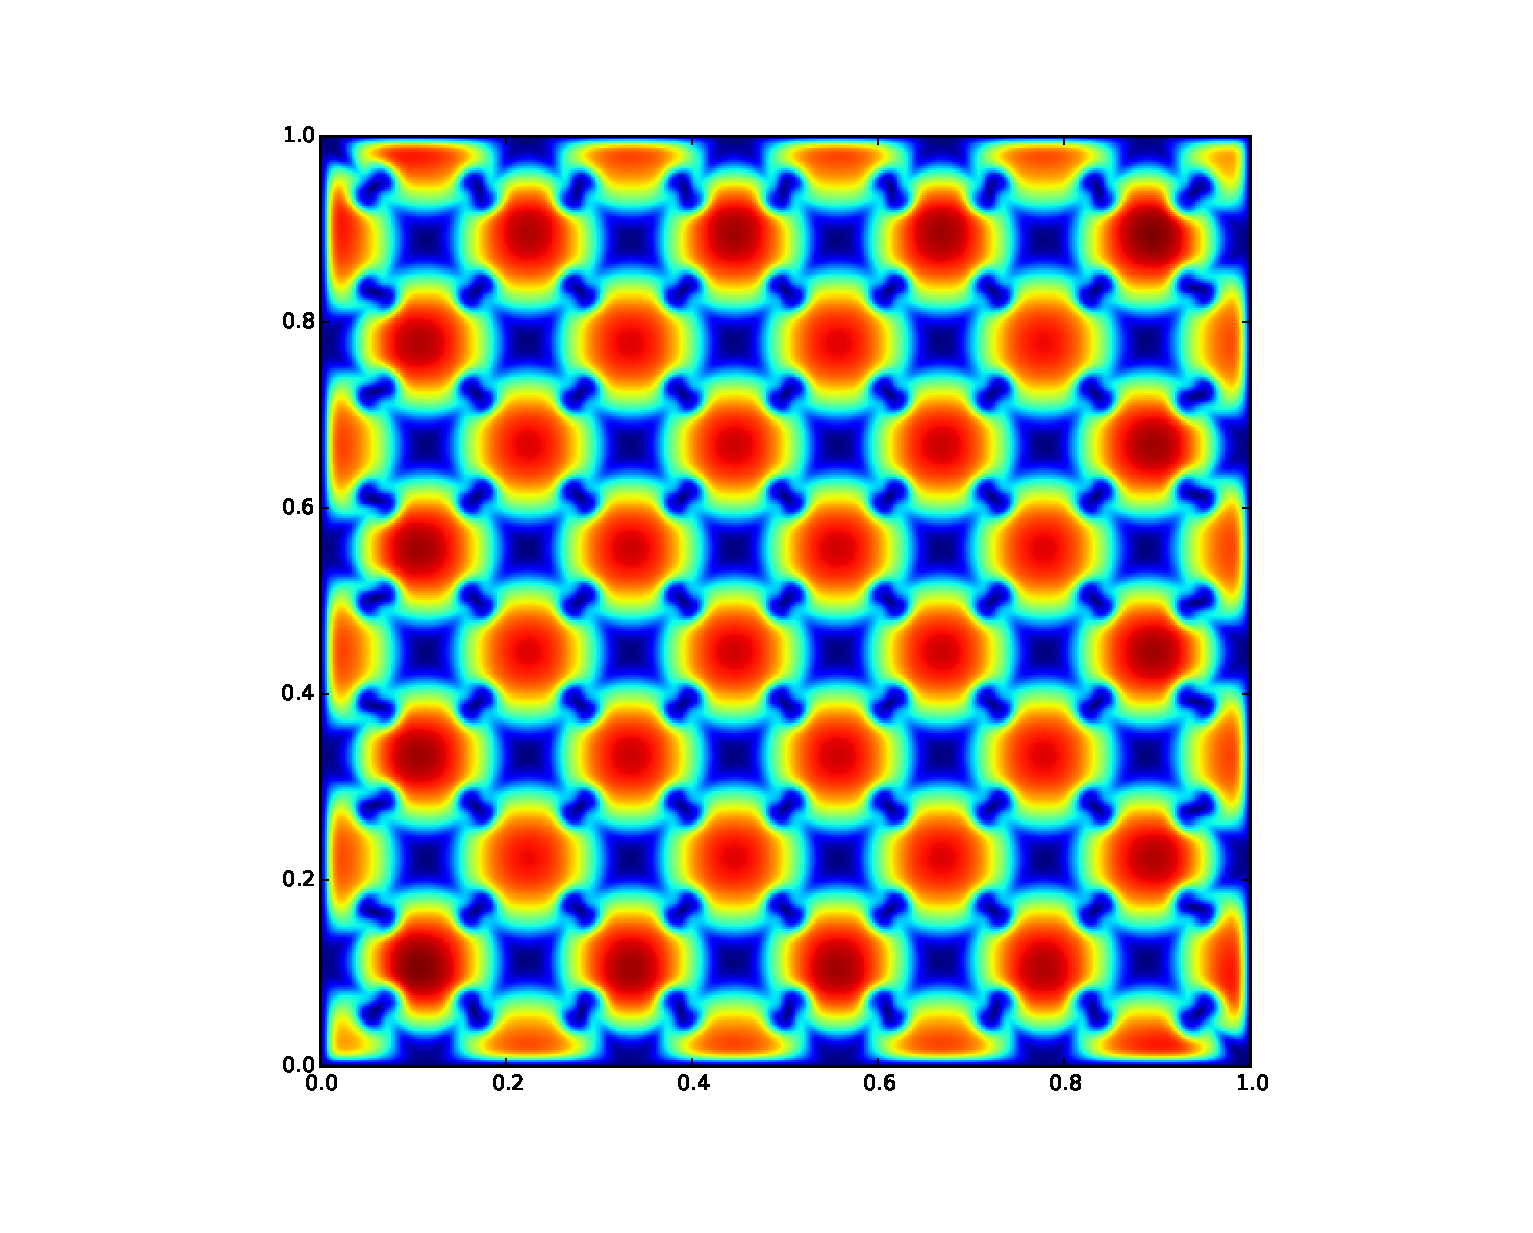
\includegraphics[width=0.66\columnwidth]{figs/dynamic_pressure-45-10}
\end{subfigure}
\caption{ \flabel{dynamic}
Dynamic pressure in the horizontal mid-plane.
}
\end{figure*}


In addition to the bubble height and vertical slices in the diagonal plane, we observe the horizontal mid-plane.
The span-wise scalar field, $\phi(x,y,0)$, exhibits plume structures that penetrate the bubble faces, as seen in \fref{phixy}.
The cause of these plumes is advection by secondary flows, as seen in \fref{secondary}.
Overlaying the pressure with the span-wise velocity reveals it to be secondary flow of the first kind: secondary flow due to span-wise pressure gradients.
The span-wise pressure gradient comes from the dynamic pressure of the rising and falling bubbles and spikes, in contrast to the stationary points at their interfaces.

The secondary flow advects mixed fluid from the interface into the centers of the bubbles and spikes.
Enhanced mixing reduces the effective Atwood number of the bubbles and spikes, but the magnitude of this effect is not clear.
As a secondary flow of the first kind, this mixing mode is present even at low Reynolds numbers.



\section{Conclusions} \slabel{concs}

The simulations described here reproduce the growth rate, stagnation velocity, and re-acceleration of the low-Atwood single mode Rayleigh Taylor instability for three experimental runs by Wilkinson and Jacobs.
These reproductions inspire confidence not only in the NekBox code, but also in the Boussinesq approximation for $A = 0.15$ and the low-Schmidt approximation.

In wall-bounded flows, the bubbles and spikes nearest to the no-slip boundaries experience lift and drag forces that slow their non-linear growth and push them towards their inner neighbors.
There is an additional effect due to the finite domain breaking one of the 4-fold symmetries from the purely periodic problem.
In the wall-bounded initial condition, one corner of the domain has an excess of bubbles while the opposite has an excess of spikes.
This sets up a long-wavelength mode across the diagonal that encourages bubble growth in one corner and discourages it in the other.

Ultimately, the bubble-bubble and spike-spike collisions may destroy the single-mode ordering of the flow at aspect ratio 5, but the onset of velocity decay may alternatively be due to the upper boundary.
If the decay is due to collisions, it would limit the use of wall-bounded flows as proxies for periodic flows to moderate aspect ratios.
The ability of wall-bounded flows to approximate periodic ones at high aspect ratio warrants further study.

In addition to causing collisions, the growing boundary layer squeezes the flow in the span-wise direction, accelerating it past its fully-periodic trajectory in the stagnation and re-acceleration phases.

The inner bubbles experience near constant acceleration from aspect ratio 2 to aspect ratio 5, with a maximum Froude number of 1.8.
This contrasts results by Ramaprabhu et al.~\cite{Ramaprabhu2012} that show saturation post-reacceleration at $\text{Fr} \approx 1$.
The saturation could be explained by excess mixing or the finite size of the domain, which extends to $h/\lambda = 6$ in their case and $9$ in ours.
Alternatively, the acceleration could be artificially sustained by the wall lift force pushing the boundary bubbles into the interior ones.

Single-mode Rayleigh-Taylor flows develop span-wise pressure gradients with local minima in bubble and spike centers and local maxima in bubble and spike corners.
The pressure drives secondary flows of the first kind in the form of vortex quads centered on bubble-spike interface centers.
These span-wise flows mix the fluid across otherwise laminar interfaces, perturbing the scalar profiles.

\section{Acknowledgements}

M. H. is grateful for useful conversations with Jeffrey Jacobs, Robert Roser, Aleksandr Obabko, Elia Merzari, Oana Marin, and Elizabeth Hicks.

M. H. acknowledges support from the Department of Energy Computational Science graduate fellowship.
This research used resources of the Argonne Leadership Computing Facility, which is a DOE Office of Science User Facility supported under Contract DE-AC02-06CH11357.




\newcommand{\pluseq}{\mathrel{+}=}

% make bold shape available for listings
\renewcommand{\ttdefault}{pcr}
\lstset{language=[90]Fortran,
  basicstyle=\ttfamily\lst@ifdisplaystyle\scriptsize\fi,
  keywordstyle=\bfseries,
  comment=[l]{!\ },
  escapechar=@,
%  numbers=left,
  tabsize=4,
}


\chapter{Efficiency of High Order Spectral Element Methods on Petascale Architectures}

% a short form should be given in case it is too long for the running head
%\titlerunning{Lecture Notes in Computer Science: Authors' Instructions}

% the name(s) of the author(s) follow(s) next
%
% NB: Chinese authors should write their first names(s) in front of
% their surnames. This ensures that the names appear correctly in
% the running heads and the author index.
%
%\author{Maxwell Hutchinson\inst{1} \and Alexander Heinecke\inst{2}  \and Hans Pabst\inst{3}  
%\and Greg Henry\inst{4}
%\and Matteo Parsani\inst{5}
%\and David Keyes\inst{5}
%}

%\institute{
%Department of Physics, University of Chicago, 5720 S. Ellis Ave, Chicago IL, 60637, USA
%Department of Physics, University of Chicago, Chicago IL, USA
%\and
%Intel Corporation, 2200 Mission College Blvd., Santa Clara CA, 95054, USA
%Intel Corporation, Santa Clara CA, USA
%\and
%Intel Semiconductor AG, Badenerstrasse 549, 8048 Zurich, Switzerland
%Intel Semiconductor AG, Zurich, Switzerland
%\and
%Intel Corporation, 2111 NE 25th Avenue, Hillsboro OR, 97124, USA
%Intel Corporation, Hillsboro OR, USA
%\and
%Extreme Computing Research Center, KAUST, Thuwal, 23955, KSA
%}


%\maketitle


\section{Abstract}
High order methods for the solution of PDEs expose a trade-off between computational cost and accuracy on a per degree of freedom basis.
In many cases, the cost increases due to higher arithmetic intensity while affecting data movement minimally.
As architectures tend towards wider vector instructions and expect higher arithmetic intensities, the best order for a particular simulation may change.

This study highlights preferred orders by identifying the high order efficiency frontier of the spectral element method implemented in Nek5000 and NekBox: the set of orders and meshes that minimize computational cost at fixed accuracy.
First, we extract Nek's order-dependent computational kernels and demonstrate exceptional hardware utilization by hardware-aware implementations.
Then, we perform production-scale calculations of the nonlinear single mode Rayleigh-Taylor instability on BlueGene/Q and Cray XC40-based supercomputers to highlight the influence of the architecture.
Accuracy is defined with respect to physical observables, and computational costs are measured by the core-hour charge of the entire application.
The total number of grid points needed to achieve a given accuracy is reduced by increasing the polynomial order.
On the XC40 and BlueGene/Q, polynomial orders as high as 31 and 15 come at no marginal cost per timestep, respectively.
Taken together, these observations lead to a strong preference for high order discretizations that use fewer degrees of freedom.
From a performance point of view, we demonstrate up to 60\% full application bandwidth utilization at scale and achieve $\approx$ 1 PFlop/s of compute performance in Nek's most flop-intense methods.

\section{Introduction}
\label{sec:introduction}
The solution of partial differential equations (PDEs) is a core problem in HPC, with particular application to computational materials science and fluid dynamics.
PDEs are solved by discrete approximation: space and time are sampled and the PDEs is translated into a relation on those samples.
From a mathematical point of view, these approximations are characterized by stability conditions and convergence rates.
Schemes which do not satisfy stability conditions usually fail catastrophically with values that diverge to infinity.
The convergence rate describes the relationship between the resolution and the error.
For a characteristic inter-sample spacing $h$, a method is of order $p$ if the error goes as $h^p$.
High order methods are schemes with convergence rates higher than third order~\cite{wang2013high}, many of which expose the order as a user input.

From a computational point of view, the approximations are characterized by sparsity, locality, and arithmetic intensity.
As the order increases, the sparsity and locality typically decrease while the arithmetic intensity increases.
The improved convergence rates are `paid for' with more floating point operations (FLOP), on a per sample basis, while, for a given error tolerance, the number of samples can be decreased.
The relationship between these computational characteristics and computational cost is complicated by features common to modern architectures: vector instructions, deep caches, and arithmetic-to-data movement imbalance.

Here, we explore the relationship between order, accuracy, cost, and architecture.
We identify the user-facing properties of high order methods: the accuracy in observables, time to solution, resource usage, and required scale.
We also identify the user-defined inputs: the physical problem, the order, the total number of samples, the number of processors, and the computer architectures.
To make the study more practical, we focus on the specific task of optimizing a study of the single-mode Rayleigh-Taylor instability (smRTI) as a parameter sweep over Grashof and Prandtl numbers.
This is a high throughput use-case, where the relevant cost is resource usage and scale is fixed with respect to the size of the problem and assumed to not be a limitation.
This leaves us with the accuracy and resource usage versus the order, number of samples, and computer architectures.

We select the NekBox version of the Nek5000 code (together: Nek), which
implements the spectral element method (SEM)~\cite{patera1984spectral} with tunable order, is known to scale to a million ranks~\cite{nekscaling}, and has been used for Rayleigh-Taylor problems in the past~\cite{hutchinson2015direct}.
NekBox takes advantage of static, uniform meshes to solve the coarse part of the preconditioner with FFTs or DCTs, improving efficiency and scalability.
We extract representative order-dependent kernels from Nek and analyze their
performance on BlueGene/Q and Cray XC40 supercomputers.

We also conduct a set of application benchmarks to measure the cost and accuracy.
The cost is computed in core-hours, in the same way most users are charged.
The accuracy is computed with respect to the smRTI's bubble height and mix volume, which are the most common observables studied in the smRTI community.
The benchmarks vary the order and total number of samples, and are conducted on the Mira and Shaheen XC40 supercomputers at Argonne Leadership Computing Facility (ALCF) and KAUST Supercomputing Laboratory (KSL), respectively.


\subsection{Outline}
In \sref{math}, we review the SEM as implemented in Nek.
In \sref{implementation}, we introduce LIBXSMM for hardware-aware implementation of Nek's performance critical kernels, and demonstrate their performance in isolation.
In \sref{benchmarks}, we perform a convergence/performance study of SEM discretizations for the smRTI problem and present full-application performance at scale.
\sref{conclusion} concludes with a discussion of preferred orders on the BlueGene/Q and Cray XC40 supercomputers. 



\section{Nek's Computational Core}
\label{sec:math}
\subsection{Governing equations and time-splitting}
Nek5000 and NekBox solve the incompressible Navier--Stokes equations:
\begin{equation}
\frac{\partial u}{\partial t} + u \cdot \nabla u = - \frac{1}{\rho} \nabla p + \nu \nabla^2 u + f \qquad
\nabla \cdot u = 0,
\end{equation}
where $u$ is the flow velocity, 
$\rho$ is the fluid density,
$p$ is the pressure,
$\nu$ is the kinematic viscosity,
and $f$ consists of user-defined forcing terms.
Additionally, Nek can solve advection-diffusion equations for scalars, such as the temperature or mass fraction:
\begin{equation}
\frac{\partial \phi_i}{\partial t} + u \cdot \nabla \phi_i =  \alpha_i \nabla^2 \phi_i + q_i,
\end{equation}
where $\phi_i$ is the scalar value, 
$\alpha_i$ is the diffusivity,
and $q_i$ is a user-defined source term, each for the $i$th scalar.

The time derivative is discretized with a backward difference formula (BDF), within which the nonlinear and forcing terms are extrapolated (EX):
\begin{equation}\elabel{semi}
\sum_{j=0}^k \frac{\beta_i}{\Delta t} M u_i^{n-j} = - \frac{1}{\rho} D_i p^n + \nu K u_i^n + \sum_{j=1}^n a_j\left[M f_i^{n-j} - (C u_i)^{n-j} \right],
\end{equation}
where $M$ is the mass matrix,
$C$ is the convection matrix,
$K$ is the stiffness matrix,
$D$ is the gradient matrix,
$i \in \{1,2,3\}$ are the spatial dimension indexes, 
$n$ is the time level index, and
$k$ is the formal order of accuracy of the BDF/EX scheme.
The pressure is decoupled from the new velocity, $u^n$, by taking the divergence:
\begin{equation} \elabel{pres}
K p^n = D_i \sum_{j=1}^n a_j F_i^{n-j},
\end{equation}
where $F_i^n = M f_i^n - (C u_i)^n$,
which results in the Poisson pressure equation.
Finally, the pressure is incorporated back into \eref{semi}:
\begin{equation} \elabel{vel}
\left[\nu K + \frac{b_0}{\Delta t} M \right] u_i^n = -D_i \frac{p^n}{\rho} + \sum_{j=1}^k \left[a_j F_i^{n-j} + \frac{b_j}{\Delta t} M u^{n-j} \right], 
\end{equation}
which results in three Helmholtz velocity equations.

\begin{comment}
The semi-discrete incompressible Navier--Stokes equations can be written as~\cite{Deville2002}:
\begin{equation} \label{eqn:NS1}
M \frac{d u_i^{n+1}}{dt} + \text{Re}~ C u_i^{n+1} + K u_i^{n+1} - D_i^T p^{n+1} =  M f_i^{n+1} \qquad \sum_i -D_i u_i^{n+1} = 0,
\end{equation}
where $M$ is the mass matrix,
$C$ is the convection matrix,
$K$ is the stiffness matrix,
$D$ is the gradient matrix,
$i \in \{1,2,3\}$ indexes spatial dimensions, and
$n$ indexes time.
The temporal derivative is expressed with the third-order backwards difference formula, and the convection operator with third-order explicit Adams-Bashforth extrapolation~\cite{Deville2002}.
The advection-diffusion equations are treated similarly, but without a pressure term, and solved first.
The forcing terms in this study depend only on $\phi$, and are evaluated directly at the next time level ($t^{n+1}$)~\cite{Tomboulides1997}.
\end{comment}

\begin{comment}
\begin{equation} \elabel{bdf}
\left(\frac{11}{6 \Delta t} M + K\right) u^{n+1}_i - D^T_i p^{n+1} = \frac{M}{\Delta t} \left(3 u^n_i - \frac{3}{2} u^{n-1}_i + \frac{1}{3} u^{n-2}_i \right) + M f_i^{n+1} - \text{Re} C u^{n+1}_i 
\end{equation}
The convection matrix and external force are extrapolated to third-order:
\begin{equation}
C u_i^{n+1} \approx \left(3 C u_i^n - 3 C u_i^{n-1} + C u_i^{n-2}\right)
\end{equation}
\end{comment}

\begin{comment}
If we group the explicit terms together as $F_i^{n+1}$ and define the Helmholtz operator $H_i = (11/6\Delta t)M + K$, 
we can re-write the governing equations in matrix form:
\begin{equation} \label{eqn:stokes}
\begin{pmatrix} \mathbf{H} & -\mathbf{D}^T \\ -\mathbf{D} & 0 \end{pmatrix} \begin{pmatrix} v^{n+1} \\ p^{n+1} \end{pmatrix} = \begin{pmatrix} \mathbf{F} \\ 0 \end{pmatrix},
\end{equation}
where $\mathbf{D} = \left[ D_1, D_2, D_3 \right]$ is the divergence matrix,
and $\mathbf{A} = \text{diag}(A_1, A_2, A_3)$ otherwise.
This expression is factored by approximating $\mathbf{H}^{-1} \approx (6 \Delta t)/11 \mathbf{M}^{-1}$:
\begin{equation} \label{eqn:NS2}
\begin{pmatrix} I & 0 \\  \frac{6 \Delta t}{11} \mathbf{D} \mathbf{M}^{-1} & I \end{pmatrix} \begin{pmatrix} \mathbf{H} & \quad-\frac{6 \Delta t}{11} \mathbf{H} \mathbf{M}^{-1} \mathbf{D}^T \\ 0 & \quad\frac{6 \Delta t}{11} \mathbf{D} \mathbf{M}^{-1} \mathbf{D}^T \end{pmatrix} \begin{pmatrix} v^{n+1} \\ p^{n+1} \end{pmatrix} \approx \begin{pmatrix} \mathbf{F} \\ 0 \end{pmatrix}.
\end{equation}
Introducing a compressible intermediate velocity $\hat{v}$, and its divergence:
\begin{equation} \label{eqn:NS3}
\begin{pmatrix} I & 0 \\ \frac{6 \Delta t}{11} \mathbf{D} \mathbf{M}^{-1} & I \end{pmatrix}  \begin{pmatrix} \hat{v} \\ \nabla \cdot \hat{v} \end{pmatrix} = \begin{pmatrix} \mathbf{F} \\ 0 \end{pmatrix} \qquad 
\begin{pmatrix} \mathbf{H} & -\frac{6 \Delta t}{11} \mathbf{H} \mathbf{M}^{-1} \mathbf{D}^T \\ 0 & \frac{6 \Delta t}{11} \mathbf{D} \mathbf{M}^{-1} \mathbf{D}^T \end{pmatrix} \begin{pmatrix} v^{n+1} \\ p^{n+1} \end{pmatrix} \approx \begin{pmatrix} \hat{v} \\ \nabla \cdot \hat{v} \end{pmatrix}.
\end{equation}

The scheme in \eref{NS3} represents a sequence of solves:
\begin{inparaenum}[\itshape a\upshape)]
\item explicit convection $\hat{v} = F$;
\item Poisson pressure equation $\bigtriangleup p^{n+1} = \nabla \cdot \hat{v}$; and
\item Helmholtz velocity equation $H v_i^{n+1} = \hat{v}_i - \nabla_i p^{n+1}$.
\end{inparaenum}
\end{comment}

These steps are the core of Nek5000 and NekBox: the explicit calculation of
right-hand sides, a Poisson solver for the pressure, \eref{pres}, and a Helmholtz solver for the three components of the velocity, \eref{vel}.

\subsection{Spectral element method}
Nek5000 and NekBox implement SEM: a two-level discretization constructed from tensor products of Gauss-Lobatto-Legendre (GLL) quadrature points within elements and continuity across elements, forming a mesh.
Fields are represented as
\begin{equation}
u(x,y,z) = \sum_{i=0}^p \sum_{j=0}^p \sum_{k=0}^p \tilde{u}_{i,j,k,e} h_i(x) h_j(y) h_k(z), 
\end{equation}
where $p$ is the polynomial order of the method,
$e(x,y,z)$ is the index of the element in the mesh,
and $h_i(x)$ is the $i$th Lagrange polynomial through the GLL points of element $e$.
The choice of Lagrange polynomials leads to diagonal mass matrices and related geometric factors.
The spectral basis within each element enjoys exponential convergence with respect to the polynomial order.
GLL points do not sample space uniformly, so concatenating elements is more effective at reducing grid spacing than increasing spectral order.
Many small elements are also better able to match complex geometries than fewer larger ones.
The spectral element method is able to satisfy both the demand for geometric flexibility with quasi-uniform coverage and spectral convergence, but the particular choice of the spectral order versus the number of elements can be difficult to optimize.

In SEM, operators are written as the product of a local operator and \textit{direct stiffness summation}, which enforces continuity at the shared element boundaries.
The local operators are decomposed into tensor products of 1D operators.
The general form of an operator $A$ is:
\begin{equation}
A = (A_x \times I_y \times I_z) + (I_x \times A_y \times I_z) + (I_x \times I_y \times A_z),
\end{equation}
where $A_x, A_y, A_z$ are 1D projections of the operator $A$ and $I$ is the
identity matrix.
In this way, linear operators from $R^{N \times N \times N} \rightarrow R^{N \times N \times N}$ can be evaluated in $O(N^4)$ operations instead of $O(N^6)$~\cite{tufo1999terascale}.
This reduces the arithmetic intensity of operator evaluation in SEM to $O(p)$.

\subsection{Computational profile}
The spectral element method, as implemented in Nek5000 and NekBox, spends its time in three computational motifs: sparse communication, vector-vector, and matrix-matrix.
The sparse communication comes from the direct stiffness summations and the coarse part of the pressure preconditioner.
The vector-vector workload comes from inner products in the solvers and frequent rescaling by geometric factors, which are shaped like the diagonal mass matrix.
The matrix-matrix workload comes from local operator evaluation.

The direct-stiffness summation is handled by a stand-alone library~\cite{ivanov2015evaluation,otten2016}. 
In Nek, the pressure solve takes roughly 30\% of the run-time, distributed between operator application, inner products, and the preconditioner.
The preconditioner is multigrid with a local additive Schwarz part and the global coarse part~\cite{lottes2005hybrid}.
In NekBox, the coarse part of the pressure preconditioner is solved directly with FFTs or fast cosine transforms, and typically takes less than 5\% of the total runtime.
Local communication makes up a small portion of NekBox's run time at moderate numbers of points per processor, and Nek5000 and NekBox weak scale effectively to millions of ranks~\cite{hutchinson2015direct}.

The efficiency of the vector-vector computation is generally left to the compiler, aided by aggressive loop merging in the solvers.
For architectures that support them, the compiler needs help issuing non-temporal stores, which are performance optimal only if the working set is larger than the last level cache.
These stores are used in parts of the solver and local element evaluation, and are discussed further in \sref{implementation}.

Matrix-matrix is the most accessible and performance critical portion of the workload.
In particular, it is the only part of Nek that depends on the order, holding the
total degrees of freedom (DOFs) fixed.

\subsection{Order-dependent kernels}
\label{sec:operators}
There are two matrix-matrix routines that sit inside of the iterative solvers: the Helmholtz operator and a basis transformation.

The Helmholtz operator is found on the left-hand side of \eref{pres} and \eref{vel}:
$$ H u = (h_1 K + h_2 M) u, $$
where the special case of $h_2 = 0$ is the Poisson operator.
\begin{algorithmic}[1] \small
\Procedure{Local Helmholtz operator}{$Hu, u, h_1, h_2$}
\State $(H u)_{i,j,k} \gets (G_x)_{i,j,k} * \sum_l (K_x)_{i,l} u_{l,j,k} $
\Comment {matrix-multiply size $(p^2,p,p)$}
\For{$k =0 \to p$}
\State $(Hu)_{i,j,k} \pluseq (G_y)_{i,j,k} * \sum_l (K_y)_{j,l} u_{i,l,k}  $
\Comment {matrix-multiply size $(p,p,p)$}
\EndFor
\State $(Hu)_{i,j,k} \pluseq (G_z)_{i,j,k} * \sum_l (K_z)_{k,l} u_{i,j,l}  $
\Comment {matrix-multiply size $(p,p^2,p)$}
\State $(Hu)_{i,j,k} \pluseq h_1 (Hu)_{i,j,k} + h_2 M_{i,j,k} u_{i,j,k} $
\EndProcedure
\end{algorithmic}
$G$ is a constant diagonal matrix derived from geometric terms and subscripts within parenthesis refer to spatial directions.
Matrix sizes are given in BLAS notation: rows in result, columns in result, inner dimension.
%The Helmholtz operator has an arithmetic intensity of $(p/3 + 1)$ floating point operations per load.

The basis transformation is used to diagonalize the local Poisson operator in the overlapping Schwarz preconditioner, to restrict and interpolate the solution and residual in the multigrid preconditioner, and to dealias the convection operator.
\begin{algorithmic}[1]
\Procedure{Transform}{$v,u$}
\State $f_{i,j,k} \gets \sum_l (A_x)_{i,l} u_{l,j,k}$
\Comment {matrix-multiply size $(p^2,p,p)$}
\For{$k =0 \to p$}
\State $g_{i,j,k} \gets \sum_l (A_y)_{j,l} f_{i,l,k}$
\Comment {matrix-multiply size $(p,p,p)$}
\EndFor
\State $v_{i,j,k} \gets \sum_l (A_z)_{k,l} g_{i,j,l}$
\Comment {matrix-multiply size $(p,p^2,p)$}
\EndProcedure
\end{algorithmic}

%Although it is not generally called from within any of the iterative solvers, the gradient operator is performance critical because it is %used to compute the dealiased convection operator in a space $(3/2)^3$ times larger than the normal basis and the pressure %contribution to the right hand sides of the solves.
%\begin{algorithmic}[1]
%\Procedure{Gradient}{$ux,uy,uz,u$}
%\State $ux_{i,j,k} \gets \sum_l Dx_{i,l} u_{l,j,k}$
%\Comment {matrix-multiply size $(p^2,p,p)$}
%\For{$k =0 \to p$}
%\State $uy_{i,j,k} \gets \sum_l Dy_{j,l} u_{i,l,k}$
%\Comment {matrix-multiply size $(p,p,p)$}
%\EndFor
%\State $uz_{i,j,k} \gets \sum_l Dz_{k,l} u_{i,j,l}$
%\Comment {matrix-multiply size $(p,p^2,p)$}
%\EndProcedure
%\end{algorithmic}



\section{Kernel Analysis and Optimization}
\label{sec:implementation}
%Having Nek's mathematical description of \sref{math} in mind, we can see that modern compilers 
%and math libraries are challenged by Nek's small matrix products and non-temporal vector and element
%updates. 
%In the following paragraphs we address the optimizations of both and close this section by a performance
%discussion of the previously identified matrix-matrix kernels carried out via proxy applications. 

\subsection{Small Matrix Multiplications}

The implementation of fast matrix multiplications, i.e., the BLAS library's GEMM routines, and dense linear algebra more generally is one of computer science's best studied fields. 
However, large matrices~\cite{Goto:2008:AHM:1356052.1356053} have been the primary focus and, as a result, vendor-tuned BLAS implementations do not provide optimal performance when used for the small GEMMs in Nek. 
Several BLAS libraries recently introduced so-called batched interfaces to speed-up series of independent and small multiplications by exploiting parallelism and amortizing calling overheads~\cite{mklbatch}. 
As Nek performs dependent GEMMs within each element, batched execution would necessarily be inter-element,  inhibiting important caching optimization and consuming significantly more memory bandwidth. 
Therefore, most of Nek's computer science related work was devoted on speeding up small GEMMs~\cite{Shin:2010:SUN:1810085.1810120}.
Parts of Nek5000 and the related NekCEM codes have been independently ported to OpenACC~\cite{markidis2015openacc, otten2016} to speed-up small GEMMs.

Today, Nek5000 and NekBox ship with a FORTRAN-based matrix-matrix implementation called \texttt{mxm\_std}.
By default, \texttt{mxm\_std} explicitly defines multiple interfaces corresponding to values of the inner dimension $k$, and provides unrolled FORTRAN primitives to the compiler.
 For IBM's BlueGene series, common sizes are manually implemented for best performance in FORTRAN assembly-intrinsics in \texttt{mxm\_bgq}. 
Similarly, \texttt{mxm\_std} features some special case optimizations targeting AMD's Opteron processor, which is used in the United States' largest system, Titan, at Oak Ridge National Laboratory.

In order to ensure the best possible performance on a range of modern Intel processors, featuring different versions of Advance Vector Extensions (AVX) instructions, we would need to conduct a long and complicated tuning effort of Nek's \texttt{mxm\_std} akin to the narrow customizations already present.
Instead, we integrated an early prototype of the LIBXSMM library~\cite{LIBXSMM,sc15poster} into NekBox. 
LIBXSMM provides highly-optimized single-threaded small matrix-multiplication routines tuned for all recent Intel processors. 
It is already successfully used in the quantum chemistry application CP2K and high-order finite element seismic wave equation solver SeisSol~\cite{breuer15high-order}. 

In contrast to \texttt{mxm\_std}, LIBXSMM creates a specific kernel implementation for each small matrix multiplication size and optimizes that kernel specifically for each set of vector extensions.
Each kernel is composed from a-priori known and best-performing basic blocks.  
Remainder handling can be performed either explicitly by application-side padding or internally by slightly less efficient fill-in basic blocks. 
We rely on the latter in our integration of LIBXSMM into NekBox. 

We leverage LIBXSMM's experimental just-in-time (JIT) compilation feature to adapt at runtime to Nek's spectral order. 
The JIT feature generates a small matrix multiplication when its size is requested for the first time and caches compiled code until the application process is terminated. 
Additionally, LIBXSMM can expose the function pointer to the application to bypass future dispatches when call patterns are simple. 

As an example, we provide the integration of LIBXSMM into NekBox's local Helmholtz kernel from \sref{operators} in \lref{int_axhm}.
This fragment is called within a loop over elements that is typically long enough to amortize overheads. 
When entering the element-local operator for the very first time, we request the required kernels from the LIBXSMM library, which JIT compiles them internally, and store the corresponding functions pointers into persistent variables to avoid dispatching in subsequent calls. 
Compared to the pseudo-code fragment, cf.~\ref{sec:operators}, we use temporary buffers to separate matrix-matrix from vector-vector operations, which are performed in one step at the end of each element.
The other common matrix-matrix motifs, basis transformation in particular, are optimized analogously. 

\begin{lstlisting}[float,
  caption={Integration of LIBXSMM into NekBox's element-local Helmholtz operator. \texttt{xmm1, xmm2, xmm3} are persistent
  functions pointers to amortize LIBXSMM's dispatching overhead. The \texttt{libxsmm\_dispatch} call JITs the requested kernel and 
  populates the persistent function pointers.},
  label=lst:int_axhm]
  logical, save :: init = .false.
  type(LIBXSMM_DMM_FUNCTION), save :: xmm1, xmm2, xmm3

  ! lazy initialization of function-private function pointers
  ! to eliminate dispatching overhead
  if (.not. init) then
    call libxsmm_dispatch(xmm1, nx, ny*nz, nx, 1.0_dp, 0.0_dp)
    call libxsmm_dispatch(xmm2, nx, ny, ny, 1.0_dp, 0.0_dp)
    call libxsmm_dispatch(xmm3, nx*ny, nz, nz, 1.0_dp, 0.0_dp)
    init = .true.
  endif

  ! element-local operation
  call libxsmm_call(xmm1, C_LOC(wddx), C_LOC(u(1,1,1)), C_LOC(work1))
  do iz=1,nz
      call libxsmm_call(xmm2, C_LOC(u(1,1,iz)), C_LOC(wddyt), C_LOC(work2(1,1,iz)))
  enddo
  call libxsmm_call(xmm3, C_LOC(u(1,1,1)), C_LOC(wddzt), C_LOC(work3))

  ! element update
  au(:,:,:) = h1* ( work1*gx + work2*gy + work3*gz ) + h2*b*u
\end{lstlisting}

\subsection{Enhancing Element Update Performance by Streaming Stores}
Caches in Intel processors are designed as write-back caches with read-for-ownership (RFO).
Therefore, writing to a vector in main memory costs two operations: a load into the cache and the write.
Nek performs many such element updates, cf. \lref{int_axhm}, and long vector updates in linear solvers.
Compiling the Helmholtz element update leads to 5 streams being
explicitly read (\texttt{gx, gy, gz, b, u}), one RFO of \texttt{au} and one write of \texttt{au}. As we stream through all elements
the RFOs are harmful for two reasons: a) they consume bandwidth
and therefore can cause a $\approx$ 16\% performance drop; 
and b) they unnecessarily occupy cache space and might  
evict useful data. 

Since the SSE2 instruction set, the Intel architecture offers so-called non-temporal stores (NTS).
These special instructions write data directly into main memory without generating RFOs and consuming cache.
They operate best when being executed on vector-length aligned addresses, as cache-line splits are impossible. 
The compiler cannot fulfill the alignment requirement for all orders, because Nek stores field data compactly, which prohibits semi-automatic generation of NTS.
Therefore, we implemented a FORTRAN interface module with a C-backend and x86 intrinsics that applies loop-peeling to leverage
NTS for the majority of stores in long, potentially unaligned updates. 
This module covers the important kernels of Nek by offering NTS-enhanced primitives to: a) set an 1d-array to a fixed value b) copy an 1d-array c) multiply component-wise an 1d array, and d) perform the Helmholtz element update, including the special case of the Poisson operator, $h_2 = 0$. For case b), Listing~\ref{lst:streamcopy} depicts Intel AVX2 code.

\begin{lstlisting}[
  float,
  language=C++,
  label={lst:streamcopy},
  caption={Loop peeling approach including determining the middle section for which aligned NTS instructions can be used.}
]{}
void stream_vector_copy( const double* i_a,
                         double*       io_c,
                         const int     i_length) {
  int l_n = 0;
  int l_trip_prolog = 0;
  int l_trip_stream = 0;
  
  /* init the trip counts to determine aligned middle section */
  stream_init( i_length, (size_t)io_c, &l_trip_prolog, &l_trip_stream );

  /* run the prologue */
  for ( ; l_n < l_trip_prolog;  l_n++ ) {
    io_c[l_n] = i_a[l_n];
  }
  /* run the bulk, using streaming stores */
  for ( ; l_n < l_trip_stream;  l_n+=8 ) {
    _mm256_stream_pd( &(io_c[l_n]),   _mm256_loadu_pd(&(i_a[l_n]))   );
    _mm256_stream_pd( &(io_c[l_n+4]), _mm256_loadu_pd(&(i_a[l_n+4])) );
  }
  /* run the epilogue */
  for ( ; l_n < i_length;  l_n++ ) {
    io_c[l_n] = i_a[l_n];
  }
}
\end{lstlisting}

\subsection{Discussion of Performance Reproducers}
In order to analyze the performance of LIBXSMM integration and the NTS module,
we have implemented standalone reproducers of the identified small matrix multiplication motifs. 
They are included in the LIBXSMM library as examples and performance tests.
In contrast to NekBox, they are parallelized via OpenMP instead of MPI, but the performance agrees within 10\% of a full NekBox execution at scale. 
We used a single node of the Cray XC40 and BlueGene/Q, cf. \sref{arch}, for generating performance data in this section.

\fref{axhm} compares the performance of Intel MKL 11.2.1, Nek's own \texttt{mxm\_std}, and LIBXSMM
with and without non-temporal stores. 
For all element sizes, LIBXSMM offers the best performance, but the difference for orders $\leq 16$ are very small as the execution is heavily memory bandwidth bound. 
A significant boost is possible by leveraging NTS: we are able to sustain 100\% of the STREAM triad 
bandwidth (101.6\,GiB/s) up to an element size of 16. 
For larger problems, the small GEMM performance is more important. 
Here LIBXSMM is up to 2$\times$ faster than \texttt{mxm\_std} und up to 40\% faster than Intel MKL. 

In case of very low orders the benefit of NTS is greater than 16\%, which we attribute to NTS avoiding cache pollution. 
For medium sized orders we exactly see the expected 16\%,
and large problems have additional bandwidth available such that RFOs are less harmful.
 
\begin{figure}[!t]
\centering
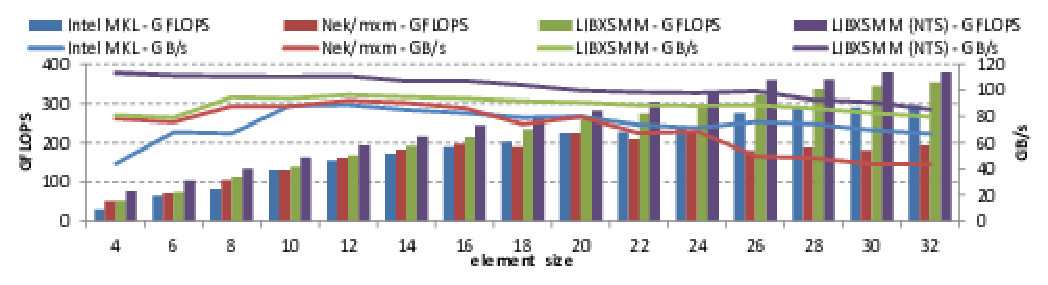
\includegraphics[width=1.0\textwidth]{gfx/axhm}
\caption{
Performance of the Helmholtz reproducer running on a single node of Shaheen for different implementation of small matrix multiplications. 
NTS denotes the usage of the non-temporal store optimized module.}
\label{fig:axhm}
\end{figure}

The performance numbers for the basis transformation on Shaheen are comparable to the Helmholtz operator and 
therefore not plotted. 
To summarize them, LIBXSMM-based GEMMs are the fastest and, due to higher computational demand, NTS are only important of for very small 1d sizes.
LIBXSMM is able to achieve 50\% of maximum floating-point performance for moderate orders.
LIBXSMM ranges from 4$\times$ faster than \texttt{mxm\_std} and Intel MKL at the smallest order to 40\% faster at the largest.


The performance of the Helmholtz kernel is representative of the basis transformations kernel on Mira as well.
To compare with Shaheen, \fref{axhm_mira} repeats the Helmholtz operator reproducer experiment
on a single node of Mira. 
IBM ESSL version 5.1.1 is used as the vendor library in place of Intel MKL.
In place of LIBXSMM, \texttt{mxm\_bgq}, which features QPX SIMD instructions, is used for the sizes that it supports.
When no QPX implementation is available, \texttt{mxm\_bgq} falls back to \texttt{mxm\_std}. 
Up to element size 16, Nek's \texttt{mxm\_std} and \texttt{mxm\_bgq} libraries are a better choice compared to IBM ESSL.
For larger element sizes (except 22 and 24) the performance is comparable.
However, the fraction of available bandwidth used is significantly worse than on Shaheen. 
Even at high element sizes, Shaheen is at 80\% bandwidth utilization with LIBXSMM and 50\% without, whereas Mira runs at 17\%.
The relative efficacy of \texttt{mxm\_bgq} on Mira, where available, highlights the strength of LIBXSMM: the ability to automatically issue the best available vector instructions at any size.


\begin{figure}[!t]
\centering
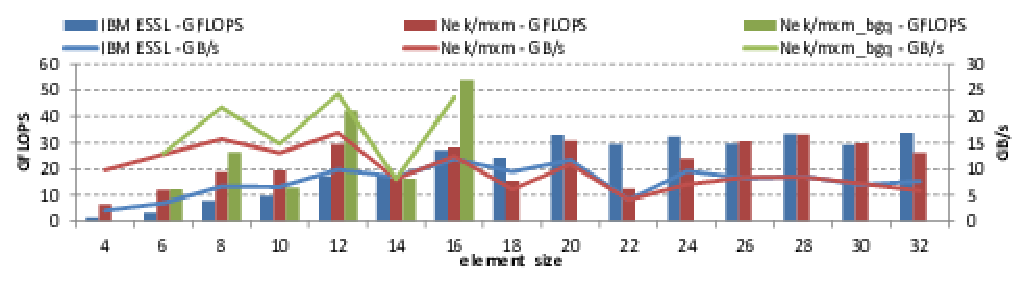
\includegraphics[width=1.0\textwidth]{gfx/axhm_mira}
\caption{
Performance of the Helmholtz operator reproducer running on a single node of Mira for different implementation of small matrix multiplications.}
\label{fig:axhm_mira}
\end{figure}

\fref{rstr} depicts corresponding performance numbers for the basis transformation reproducer in three use cases: a) unitary transformation from element size to element size, b) prolongation/dealiasing from 1d size to $(3/2)$ the element size, and c) restriction/aliasing from 1d size to (2/3) the element size.
Note that the $(3/2)$ factor implies some dimensions are significantly larger then the element size shown on the x-axis.

As with the Helmholtz reproducer, the LIBXSMM-based executions are the fastest and due to higher
computational demand; 
NTS are only important of for very small 1d sizes. 
LIBXSMM is able to achieve 50\% of maximum floating-point performance for medium sized orders
In direct comparison to \texttt{mxm\_std} and Intel MKL, the speed-up of LIBXSMM varies between close to 4$\times$ at very small order to roughly 40\% at very large order.

\begin{figure}[!t]
\centering
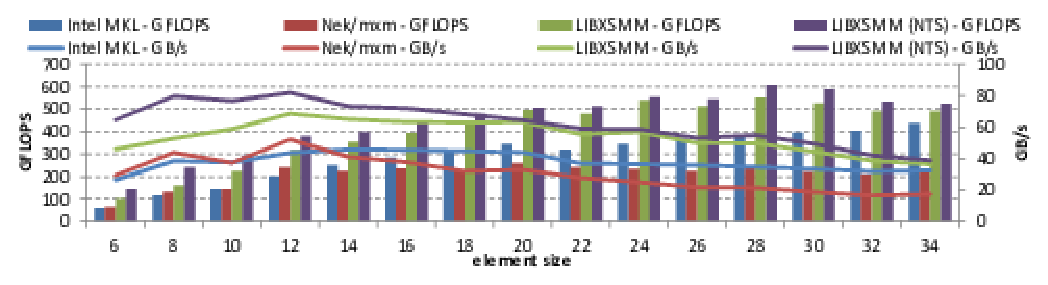
\includegraphics[width=1.0\textwidth]{gfx/rstr}   
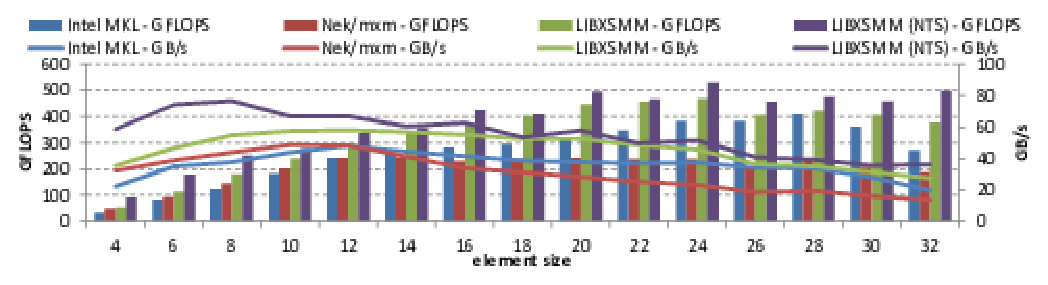
\includegraphics[width=1.0\textwidth]{gfx/rstr_fwd}
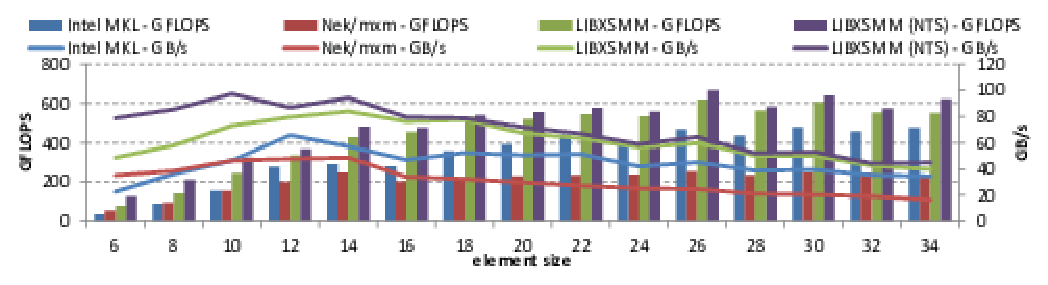
\includegraphics[width=1.0\textwidth]{gfx/rstr_rev}
\caption{Performance of the basis transformation reproducers using different implementation for the 
small matrix multiplications. NTS denotes the usage of the aforementioned non-temporal store optimized module. The top plot
shows the diagonalization in the local Poisson operator, the middle one the prolongation and the bottom one the restriction case.}
\label{fig:rstr}
\end{figure}

%Finally, the gradient reproducer's performance is plotted in \fref{grad}.
%The floating point load is very similar to Helmholtz, but only one element is read, instead of five, and three elements are written, %instead of one.
%While both are bandwidth bound, the higher write load makes gradient more sensitive to RFO.
%NTS doubles the performance in case of small and medium sized orders. 
%Therefore, without NTS, the high bandwidth cost masks the floating point cost and it does not matter which matrix-matrix routines are %used.
%Even so, LIBXSMM results in the fastest execution.
%
%\begin{figure}[!t]
%\centering
%\includegraphics[width=1.0\textwidth]{gfx/grad}
%\caption{Performance of the gradient operator reproducer using different implementation for the small matrix 
%multiplications. NTS denotes the usage of the aforementioned non-temporal store optimized module.}
%\label{fig:grad}
%\end{figure}


\section{Scenarios and Performance}
\label{sec:benchmarks}
\subsection{Architectures} \slabel{arch}

We run on two supercomputers: Mira at the ALCF and Shaheen XC40 at the KSL.
Mira is a IBM BlueGene/Q with 49,152 nodes.
Each node has 16 cores with 4 hardware threads per core and can support 204.8
GFLOPS and 30 GiB/s main memory bandwidth, measured by~\cite{McCalpin2007}.
Shaheen is a Cray XC40 with 6144 nodes.
Each node has two Intel\textsuperscript{\textregistered}
Xeon\textsuperscript{\textregistered} E5-2698v3 (code-named Haswell) processors
with 16 cores each and can support around 1177.6 GFLOPS and 101.6 GiB/s main memory bandwidth, measured by~\cite{McCalpin2007}.
Shaheen's cores therefore have 2.9$\times$ the floating point and 1.7$\times$ the memory bandwidth of Mira's BlueGene/Q cores.

\subsection{Single mode Rayleigh-Taylor instability}

The Rayleigh-Taylor instability (RTI) occurs when the pressure and density gradients point in opposite directions, as in the canonical case of a heavy fluid supported on top of a lighter fluid in a gravitational field.
The Rayleigh-Taylor growth rate is an increasing function of the wave-number, up to a viscous cutoff, making the smallest scales grow fastest.
Because energy is pumped into the system at small scales, the RTI is notoriously difficult to model numerically~\cite{Dimonte2004}.

The RTI describes how the dense fluid is pushed through and mixes with lighter fluid.
This dynamic mixing process is essential to the behavior of flows found in exploding stars~\cite{Bell2004}, the oceans and atmosphere~\cite{Linden1973}, and inertial confinement fusion.
In the latter case, dense plastic ablator is pushed into and mixed with the lighter hydrogen fuel.
The carbon-laden ablator radiates energy much more quickly than the fuel, reducing hot-spot temperature and preventing ignition.
The study of the RTI and related mixing is a priority research direction for inertial confinement fusion performance~\cite{Gocharov2012}.

Nek5000 and NekBox~\cite{NekBox} are used to model the incompressible Boussinesq equations, which approximate the RTI at low density contrasts:
\begin{align}
\frac{\partial u}{\partial t} + u \cdot \nabla u &= - \nabla p + \nu \nabla^2 u + \tilde{g} T \\
\frac{\partial T}{\partial t} + u \cdot \nabla T &= \alpha \nabla^2 T \\
\nabla \cdot u &= 0,
\end{align}
where $T$ is a scalar that can be interpreted as a temperature, 
in which case $\alpha$ is the thermal diffusivity 
and $\tilde{g}$ is the product of the gravitational acceleration and the thermal expansion coefficient.

The single-mode Rayleigh-Taylor instability (smRTI) restricts the initial perturbation of the interface to be sinusoidal, and is generally considered in periodic span-wise boundary conditions:
\begin{equation} \elabel{IC}
T(x,y,z,0) = A\cdot \text{erf}\left[\frac{z + a_0 \cos(2 \pi x/\lambda) \cos(2 \pi y/\lambda)}{\delta}\right],
\end{equation}
where $A \in (0,1]$ is the Atwood number,
$\lambda$ is the wavelength, 
$a_0$ is the initial interface amplitude, and
$\delta$ is the initial interface width.
This simplification allows the problem to be defined by only two dimensionless numbers in the limit of $a_0, \delta \rightarrow 0$, the Grashof number (Gr) and the Prandtl number (Pr):
\begin{equation}
\text{Gr} = \frac{A \tilde{g} \lambda^3}{\nu^2},  \qquad \text{Pr} = \frac{\nu}{\alpha}.
\end{equation}

Even under these simplifications, the late-time behavior is not well understood.
Experiments are prone to spurious low-wavelength modes that dominate the dynamics at late times, while the cost of direct numerical simulations is quadratic with the domain's aspect ratio.

It would be valuable to systematically sample the Grashof-Prandtl space with high fidelity simulations at late-time/high-aspect-ratio to better inform experimental design and model development.
Such a study would be very expensive, so it is important to select a cost-minimizing strategy.

We take this problem, the selection of a cost-minimizing strategy for the late-time smRTI, as our motivation.
In addition to the isolated reproducers discussed in \sref{implementation}, we present NekBox application benchmarks based on smRTI with typical Nek settings.
The aim of these benchmarks is to identify minimum cost discretizations that attain a given accuracy.

The benchmarks are conducted for combinations of the element size taken from $\{4, 6, 8, 10, 12, 14, 16, 32\}$ and span-wise mesh size taken from $\{2, 4, 8, 12, 16, 24, 32, 48, 64, 96, 128\}$.
The total number of points ranges from around 1 million to 4 billion.
The problem is weak-scaled: the number of elements per rank is chosen as to consume approximately half of the available main memory, or around 16k and 262k points per rank on Mira and Shaheen, respectively.
The problems are constrained to fill an integer number of nodes, which puts a lower bound on the mesh size and excludes some cases that would partially fill nodes.
The domain is a box with dimension $[0,.5]^2 \times [-1,1]$, and the elements are cubic.
The span-wise boundary conditions are symmetric and the vertical boundary conditions are no-slip in velocity and no-flux (insulating) in the scalar.
The initial condition is stationary in velocity with a scalar given by \eref{IC}, the Grashof number is 17,324, and the Prandtl number is 1.
The timestep is calculated based on a Courant number of $0.4$, which scales linearly with the number of elements and quadratically with the size of the element due to the spacing of the GLL nodes.
The Courant condition is defined only in a linear limit, so during the initial exponential growth regime the Courant number is computed using the stagnation velocity, $\sqrt{A \tilde{g}/(\pi \lambda)}$.


Outputs are written at regular intervals in simulated time, constant across problem sizes.
Therefore, smaller problems perform a greater share of I/O, as is the common case in CFD.
Nek5000 and NekBox write separate files for separate ranks.
The number of ranks that participate in I/O is a fixed proportion of the total number of ranks.

\begin{figure}
\begin{subfigure}[b]{0.25\textwidth}
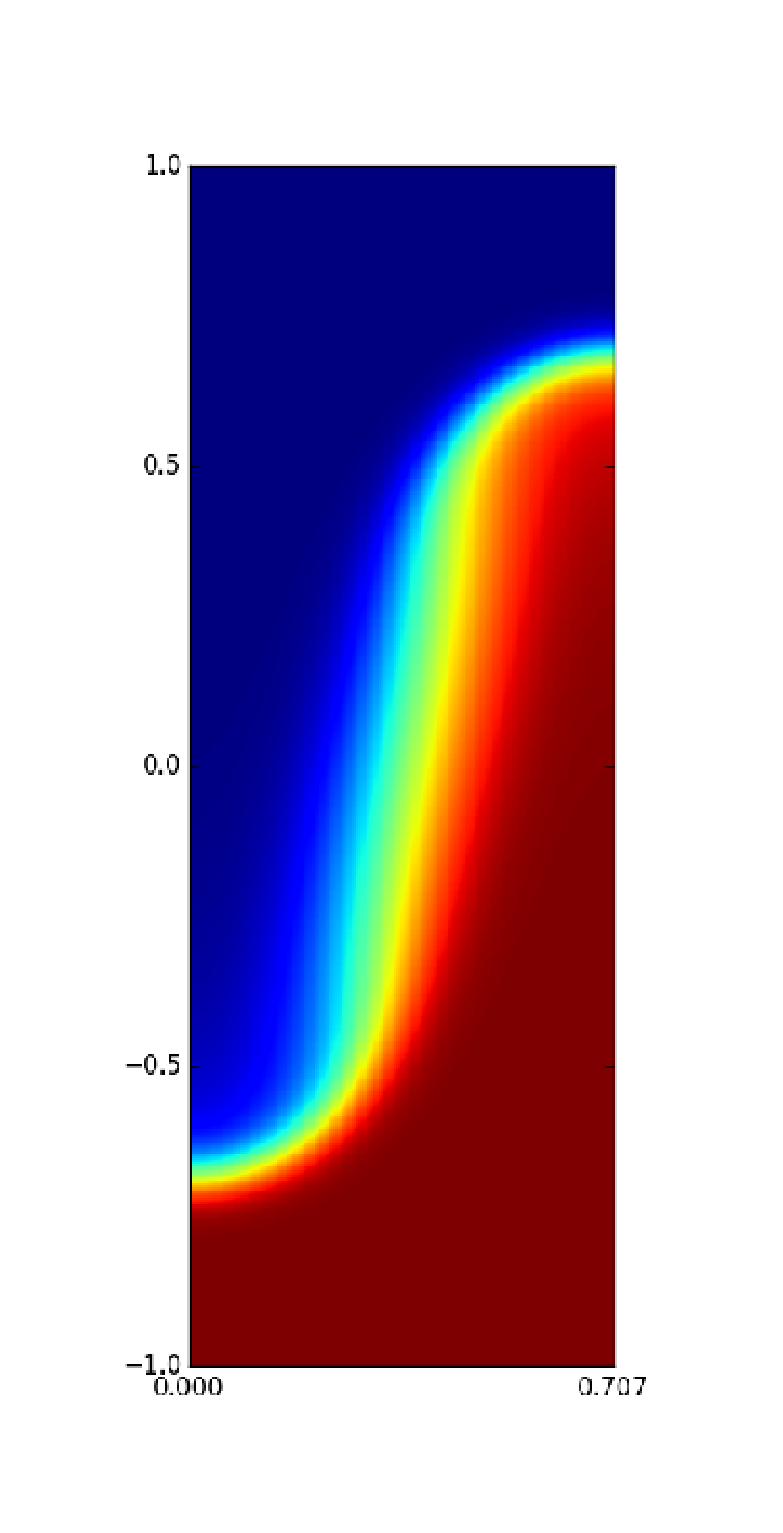
\includegraphics[width=0.25\textwidth]{gfx/cnv_o16_e32-t_yz-0033}
\end{subfigure}
\begin{subfigure}[b]{0.25\textwidth}
\includegraphics[width=0.25\textwidth]{gfx/cnv_o16_e32-w_yz-0033}
\end{subfigure}
\begin{subfigure}[b]{0.25\textwidth}
\includegraphics[width=0.25\textwidth]{gfx/cnv_o16_e32-vorticity_yz-0033}
\end{subfigure}
\begin{subfigure}[b]{0.25\textwidth}
\includegraphics[width=0.25\textwidth]{gfx/cnv_o16_e32-p_yz-0033}
\end{subfigure}
\caption{ \flabel{slices}
Scalar, velocity, vorticity, and pressure fields at end of simulation.
}
\end{figure}

Slices of the end of the simulation are shown in \fref{slices}.
Two observables are calculated in post-processing: the \textit{bubble height} and the \textit{mix volume}:
\begin{equation} \elabel{observe}
H = \sup \left\{ z : \min_{x,y} ~ T(x,y,z) < T_0\right\}, \qquad
\Theta = \int \left|T - T_0\right| dV, 
\end{equation}
where $T_0$ is the volumetric average temperature.
These two observables are common to smRTI models and lie at opposite ends of the locality spectrum: 
the bubble height is defined by the neighborhood of the bubble tip while the mix volume is an integral over the entire domain.
The root mean square error in each observable is computed over all the outputs.


\subsection{Time to accuracy}

\begin{figure}
\begin{subfigure}[t]{0.49\textwidth}
\includegraphics[width=0.49\textwidth]{gfx/combined-bw}
\caption{Bandwidth}
\end{subfigure}
\begin{subfigure}[t]{0.49\textwidth}
\includegraphics[width=0.49\textwidth]{gfx/mira_vs_haswell}
\caption{Ratio}
\end{subfigure}
\caption{ \flabel{bwcomp}
Weak scaling of bandwidth on Shaheen and Mira.
In (a), Circles and crosses indicate memory bandwidth per core on Shaheen and Mira, respectively, vs the problem size labeled by element size.
In (b), the ratio of the bandwidths are shown vs element size for common discretizations.
The solid line indicates ratio of STREAM memory bandwidth.
}

\end{figure}

For each simulation, we compute the FLOP rate and aggregate memory bandwidth.
NekBox includes explicit FLOP and memory operation counters and timers in the most performance critical regions of the code.
Memory operations are counted assuming single-element intermediate data stays in cache, and therefore does not contribute to main memory bandwidth.
These counters are consistent with those used in the reproducers.
The whole application is not covered, so the counters can be considered lower bounds on the whole-application performance.

The attained memory bandwidth per core on Shaheen and Mira are plotted in \fref{bwcomp}.
On Shaheen, bandwidth is constant with respect to the number of elements and a weak function of the order, ranging from around 65 to 75\% of peak.
On Mira, bandwidth is still constant with respect to the scale, but varies more strongly with polynomial order, especially at orders greater than 16 and those not divisible by 4.
It ranges from around 15 to 50\% of peak.
The \texttt{mxm\_bgq} library, discussed in \sref{implementation}, is used, resulting in performance spikes at QPX-supported orders, e.g. 8.

\begin{figure}
\begin{subfigure}[t]{0.49\textwidth}
\includegraphics[width=0.49\textwidth]{gfx/shaheen_H}
\caption{Shaheen}
\end{subfigure}
\begin{subfigure}[t]{0.49\textwidth}
\includegraphics[width=0.49\textwidth]{gfx/mira_H}
\caption{Mira}
\end{subfigure}

%\subfloat[][Error wrt $dt$]{\includegraphics[width=0.33\textwidth]{gfx/cnv_wrt_t}}
%\subfloat[][Shaheen ($\Theta$)]{\includegraphics[width=0.5\textwidth]{gfx/shaheen_A}}

%\subfloat[][Mira ($\Theta$)]{\includegraphics[width=0.5\textwidth]{gfx/mira_A}}

\caption{ \flabel{frontier}
Error with respect to bubble height, \eref{observe}, vs. the computational cost, in processor hours, on Shaheen (a) and Mira (b).
Points are labeled as $(p+1, e)$ pairs, where $p$ is the order, $p+1$ is the element size, and $e$ is the number of elements in one dimension.
More runs are present on Mira due to the smaller BGQ nodes evenly dividing more problem sizes.
}
\end{figure}

The accuracy is plotted versus the computational cost for a variety of discretizations in \fref{frontier}.
The error in bubble height and mix volume are strongly correlated, so only the error in the height is plotted.
As expected, doubling the the spectral order while keeping the number of elements fixed, e.g. $(4,32) \rightarrow (8,32)$ and $(8,8) \rightarrow (16,8)$, significantly improves the accuracy, but also increases the cost by 16-32$\times$.
The first 8$\times$ is due to an increase in the number of degrees of freedom, the next 2$\times$ is due to the shorter timestep, and, when compute-bound, the final 2$\times$ is due to an increase in the floating point load.
Doubling the spectral order while keeping the number of points fixed, e.g. $(16, 8) \rightarrow (32,4)$  and $(8,8) \rightarrow (16,4)$, increases the cost by 2-4x, as expected, but also improves the accuracy.
Doubling the spectral order while halving the number of points in each direction, e.g. $(8,32) \rightarrow (16,8)$ and $(14, 16) \rightarrow (28, 4)$, reduces the cost by 4-8$\times$ while maintaining or slightly improving the accuracy.

We define the \emph{efficiency frontier} as the set of discretizations that minimize computational cost for fixed accuracy or, equivalently, minimize error given fixed computational cost.
The efficiency frontiers on Mira and Shaheen are comprised of discretizations with very high orders, given our constraints.
The most efficient schemes are those with element size greater than 16, except for very low accuracy simulations.

\begin{comment}

\subsection{Order-independent timestepping}
\begin{figure}
\begin{subfigure}[t]{0.33\textwidth}
\includegraphics[width=0.49\textwidth]{gfx/shaheen_H}
\caption{Shaheen}
\end{subfigure}
\begin{figure}
\begin{subfigure}[t]{0.33\textwidth}
\includegraphics[width=0.49\textwidth]{gfx/shaheen_H}
\caption{Mira}
\end{subfigure}
\begin{figure}
\begin{subfigure}[t]{0.33\textwidth}
\includegraphics[width=0.49\textwidth]{gfx/shaheen_H}
\caption{Cost vs DOF}
\end{subfigure}



	\subfloat[][Shaheen]{\includegraphics[width=0.33\textwidth]{gfx/shaheen_cfl_H}}
\subfloat[][Mira]{\includegraphics[width=0.33\textwidth]{gfx/mira_cfl_H}}
\subfloat[][Cost vs DOF]{\includegraphics[width=0.33\textwidth]{gfx/perf_vs_dof}}
%\subfloat[][Shaheen ($\Theta$)]{\includegraphics[width=0.5\textwidth]{gfx/shaheen_A}}

%\subfloat[][Mira ($\Theta$)]{\includegraphics[width=0.5\textwidth]{gfx/mira_A}}

\caption{ \flabel{cfl3}
Error with respect to bubble height, \eref{observe}, vs. the computational cost, in processor hours, on Shaheen (a) and Mira (b).
Cost vs. total degrees of freedom (c), with circles from Mira and crosses from Shaheen.
In all cases, the ratio of timestep to maximal velocity is held fixed to match the CFL condition $C = 0.4$ in the (32,8) case, which sets the temporal error floor at the solid black line in (a) and (b).
}
\end{figure}

When using high order methods, there is often a gap between the convergence rate or the spatial and temporal discretizations.
To achieve high accuracy, it is necessary to reduce the timestep below the CFL stability condition.
Doing so decouples the number of timesteps from the element size.
Now, the computational cost depends on the order, for fixed total points, only through an increase in arithmetic intensity.
If the calculation is bandwidth-bound, then high order should come at no marginal cost.
If the calculation is compute-bound, then high order should come at linear cost, in return for exponential spatial convergence.

To demonstrate this, we reduce the time step to that of the $(32,8)$ discretization in the previous section by reducing the CFL number according to the spatial discretization.
This gives us a bound on the temporal error in $H$ of $2\times 10^{-6}$.
\fref{cfl3} plots the accuracy vs the computational cost, as in \fref{frontier} but with order-independent timestepping, along with the cost vs degrees of freedom.
We see that the most efficient calculations, those that minimize cost for a given error, are all very high order.
The cost is a strong function of the number of degrees of freedom and a weak function of the order.
On Shaheen in particular, the dependence of the cost on the order seems to be in the noise, all
runs took roughly the same computing time, independent from the chosen order.
\end{comment}

\begin{comment}
\subsection{Discussion}

\subsubsection{Time to solution}

Here, we have considered computational cost in the high-throughput context: the consumption of computational resources as measured in core hours.
Alternatively, one could consider the low-latency context: the minimum time to solution, i.e. the strong-scaling limit.
In this limit, we care about the number and computational duration of time iterations.

If we

This analysis can fail in at least three ways: a) we could saturate the network before we hit latency limits, which is unlikely given that Nek is predominantly nearest-neighbor; b) we could hit the coarse grain parallelism limit before we hit latency limits; or c) the number of iterations in the solvers could increase or decrease.

On low-latency networks, Nek5000's strong scaling limit is known to be of order 1000 grid points.
NekBox reduces the communication load, so its limit could be lower.
Therefore we expect to hit (b) at polynomial order between 10 and 16.
\end{comment}

\subsection{Whole application performance}

\begin{figure}[!t]
\centering
\includegraphics[width=0.55\textwidth]{gfx/shaheen_strong}
~
\includegraphics[width=0.42\textwidth]{gfx/shaheen_weak}
\caption{Strong scaling (left) and weak scaling (right) on Shaheen on up to 131,072  cores (2/3) of the full 7 PFLOPS machine using 
an element size of 32.
To avoid log plots we show per-core performance.}
\label{fig:shaheen_scaling}
\end{figure}

To date, our largest calculation on Shaheen occupied 131,072 cores as depicted in Fig.~\ref{fig:shaheen_scaling}
for element size 32.
NekBox achieved 197 TiB/s memory bandwidth and 290 TFLOPS in weak scaling.
This corresponds to 47.8\% of peak memory bandwidth sustained over the entire application at high order.
In case of strong scaling these numbers are slightly lower with 130 TiB/s and 195 TFLOPS. 
%This is true for both, weak and strong scaling, as Shaheen uses dynamic  node-level power capping, that kicks 
%in when more than about 1/3 of the machine is used~\cite{pedretti2015early}. This cap is most likely caused by
%the high demand of compute and bandwidth of the Helmholtz as this phase is still scaling and achieves 
However, the Helmholtz operator, as the most compute intense sub-routine, is able to achieve
up to 0.94\,PFLOPS in strong and 1.33\,PFLOPS
 in weak-scaling on 131,072 cores. %\footnote{We are currently working together with KSL to root-cause the
%power capping issues. Due to the holidays this was not possible at submission deadline.}
We also consider 65,536 cores runs, occupying 1/3 of Shaheen.
These runs achieved at least 135.6 TiB/s memory bandwidth and 184.9 TFLOPS.
This corresponds to 67.5\% of peak memory bandwidth sustained over the entire application at high order.
Finally, extrapolating to full machine, NekBox would reach at least 406.8 TiB/s and 554.6 TFLOPS. At the same scale,
a weak scaling of the Helmholtz operator would result into 1.9\,PFLOPS out of 7\,PFLOPS performance.





\section{Conclusion}
\label{sec:conclusion}
NekBox enhanced by LIBXSMM generated kernels on Shaheen XC40 executes the performance critical, order-dependent components of Nek above 80\% of peak memory bandwidth.
For comparison, compiled code on the BlueGene/Q architecture is only able to
reach 50\% of peak and for many polynomial orders operates around 30\%.
Therefore, despite only having 1.7$\times$ the memory bandwidth, Shaheen's cores
outperform Mira's cores by 3-6$\times$, with the greatest improvement at high
order and for sizes that are not divisible by the vector width, 4 in this case.
NekBox is able to scale 67.5\% utilization rates to 65,536 cores on Shaheen.

%, beyond which power throttling reduces efficiency by a factor of 2 overall. 
%However, the Helmholtz operator is relatively unaffected and able to achieve a PFLOPS of performance on 131,072 cores.

For the smRTI, the efficiency frontier, i.e., the discretizations that minimize
cost given accuracy or minimize error given cost, have polynomial orders between 15 and 31, higher than are typically used in spectral element schemes.
The presence of high order schemes on the efficiency frontier can be understood by the combination of two effects.
First, the increase in arithmetic intensity is hidden by the imbalance between floating point capabilities and memory bandwidth, providing high order at no marginal cost on a per time step basis.
Second, higher order schemes with fewer degrees are freedom are more accurate than lower order schemes with more degrees of freedom.
It is generally possible to maintain accuracy by increasing the order while decreasing the total degrees of freedom, and, consequently the total cost.

Generally the order should be chosen to be at least large enough to saturate the floating point capabilities of the architecture in the order-dependent kernels, because increasing the order to that point significantly improves accuracy at no marginal computational cost.
On BlueGene/Q, this mark is polynomial order 15, while on the Cray XC40 it is 31.

For many problems and observables, the calculation may additionally benefit from increasing the order until just before single-element operations spill out of cache.
The improvement in accuracy is exponential with the polynomial order, so the degrees of freedom needed to achieve a level of accuracy can decrease.
The increase in the cost with respect to order for compute-bound orders is linear, so if the decrease in the number of degrees of freedom needed is super-linear, the net result is a less expensive calculation.
Usage in this way, which exceeds the largest element sizes that we ran on Shaheen, warrants further study.

More generally, high order methods with high locality, the structured elements in SEM being only one example, are able to take advantage of wider vectors and higher compute to memory ratios to reach higher order at little to no marginal cost on a per-step basis.
However, increases in cost can come in through coupling to the choice of time-step and an increase in iteration counts in the solvers.
These increases can often be mitigated by reducing the total number of degrees of freedom, relative to an equivalent lower-order calculation.

The next generation will include supercomputers featuring the Xeon Phi processor code-named Knights Landing, e.g., Cori at NERSC with more than 20 PFLOPS.
As the architecture continues to evolve, we can see that updated node-level optimizations and order-sensitivity studies are key to helping scientists continue to perform large scale, high efficiency simulations. 

\section*{Acknowledgment}

This research used the resources of the Supercomputing Laboratory at the King Abdullah University of Science \& Technology (KAUST) in Thuwal, Saudi Arabia.
This research used resources of the Argonne Leadership Computing Facility, which is a DOE Office of Science User Facility supported under Contract DE-AC02-06CH11357.

We acknowledge useful conversations with
Paul Fischer, 
James Lottes,
Aleksandr Obabko,
Oana Marin,
Michel Schanen,
Scott Parker,
Vitali Morozov,
Matthew Otten,
and Robert Rosner.




\scriptsize

\noindent Optimization Notice: Software and workloads used in
performance tests may have been optimized for performance only on
Intel microprocessors.  Performance tests, such as SYSmark and
MobileMark, are measured using specific computer systems,
components, software, operations and functions.  Any change to any
of those factors may cause the results to vary.  You should
consult other information and performance tests to assist you in
fully evaluating your contemplated purchases, including the
performance of that product when combined with other products.
For more information go to http://www.intel.com/performance.

\noindent Intel, Xeon, and Intel Xeon
Phi are trademarks of Intel Corporation in the U.S. and/or other
countries.



\chapter{Conclusions}

\section{New model for low-Atwood single mode}

\section{Validation of DNS}

\section{Importance of Schmidt number}

\section{Open questions}

 % Conclusion

% Format a LaTeX bibliography
\makebibliography

% Figures and tables, if you decide to leave them to the end
%\input{figure}
%\input{table}

\end{document}


